\documentclass[12pt,a4paper,]{book}
\def\ifdoblecara{} %% set to true
\def\ifprincipal{} %% set to true
\let\ifprincipal\undefined %% set to false
\def\ifcitapandoc{} %% set to true
\let\ifcitapandoc\undefined %% set to false
\usepackage{lmodern}
\usepackage{amssymb,amsmath}
\usepackage{ifxetex,ifluatex}
%\usepackage{fixltx2e} % provides \textsubscript %PLLC
\ifnum 0\ifxetex 1\fi\ifluatex 1\fi=0 % if pdftex
  \usepackage[T1]{fontenc}
  \usepackage[utf8]{inputenc}
\else % if luatex or xelatex
  \ifxetex
    \usepackage{mathspec}
  \else
    \usepackage{fontspec}
  \fi
  \defaultfontfeatures{Ligatures=TeX,Scale=MatchLowercase}
\fi
% use upquote if available, for straight quotes in verbatim environments
\IfFileExists{upquote.sty}{\usepackage{upquote}}{}
% use microtype if available
\IfFileExists{microtype.sty}{%
\usepackage{microtype}
\UseMicrotypeSet[protrusion]{basicmath} % disable protrusion for tt fonts
}{}
\usepackage[margin = 2.5cm]{geometry}
\usepackage{hyperref}
\hypersetup{unicode=true,
            pdfauthor={Nombre Completo Autor},
              pdfborder={0 0 0},
              breaklinks=true}
\urlstyle{same}  % don't use monospace font for urls
\usepackage{natbib}
\bibliographystyle{plainnat}
\usepackage[usenames,dvipsnames]{xcolor}  %new PLLC
\IfFileExists{parskip.sty}{%
\usepackage{parskip}
}{% else
\setlength{\parindent}{0pt}
\setlength{\parskip}{6pt plus 2pt minus 1pt}
}
\setlength{\emergencystretch}{3em}  % prevent overfull lines
\providecommand{\tightlist}{%
  \setlength{\itemsep}{0pt}\setlength{\parskip}{0pt}}
\setcounter{secnumdepth}{5}
% Redefines (sub)paragraphs to behave more like sections
\ifx\paragraph\undefined\else
\let\oldparagraph\paragraph
\renewcommand{\paragraph}[1]{\oldparagraph{#1}\mbox{}}
\fi
\ifx\subparagraph\undefined\else
\let\oldsubparagraph\subparagraph
\renewcommand{\subparagraph}[1]{\oldsubparagraph{#1}\mbox{}}
\fi

%%% Use protect on footnotes to avoid problems with footnotes in titles
\let\rmarkdownfootnote\footnote%
\def\footnote{\protect\rmarkdownfootnote}


  \title{}
    \author{Nombre Completo Autor}
      \date{27/10/2017}


%%%%%%% inicio: latex_preambulo.tex PLLC

%% UTILIZA CODIFICACIÓN UTF-8
%% MODIFICARLO CONVENIENTEMENTE PARA USARLO CON OTRAS CODIFICACIONES


\usepackage[spanish,es-nodecimaldot,es-noshorthands]{babel}
\usepackage{float}
\usepackage{placeins}
\usepackage{fancyhdr}
% Solucion: ! LaTeX Error: Command \counterwithout already defined.
% https://tex.stackexchange.com/questions/425600/latex-error-command-counterwithout-already-defined
\let\counterwithout\relax
\let\counterwithin\relax
\usepackage{chngcntr}
%\usepackage{microtype}  %antes en template PLLC
\usepackage[utf8]{inputenc}
\usepackage[T1]{fontenc} % Usa codificación 8-bit que tiene 256 glyphs

%\usepackage[dvipsnames]{xcolor}
%\usepackage[usenames,dvipsnames]{xcolor}  %new
\usepackage{pdfpages}
%\usepackage{natbib}




% Para portada: latex_paginatitulo_mod_ST02.tex (inicio)
\usepackage{tikz}
\usepackage{epigraph}
\renewcommand\epigraphflush{flushright}
\renewcommand\epigraphsize{\normalsize}
\setlength\epigraphwidth{0.7\textwidth}

\definecolor{titlepagecolor}{cmyk}{1,.60,0,.40}

%\DeclareFixedFont{\titlefont}{T1}{ppl}{b}{it}{0.5in}

% \makeatletter
% \def\printauthor{%
%     {\large \@author}}
% \makeatother
% \author{%
%     Author 1 name \\
%     Department name \\
%     \texttt{email1@example.com}\vspace{20pt} \\
%     Author 2 name \\
%     Department name \\
%     \texttt{email2@example.com}
%     }

% The following code is borrowed from: https://tex.stackexchange.com/a/86310/10898

\newcommand\titlepagedecoration{%
\begin{tikzpicture}[remember picture,overlay,shorten >= -10pt]

\coordinate (aux1) at ([yshift=-15pt]current page.north east);
\coordinate (aux2) at ([yshift=-410pt]current page.north east);
\coordinate (aux3) at ([xshift=-4.5cm]current page.north east);
\coordinate (aux4) at ([yshift=-150pt]current page.north east);

\begin{scope}[titlepagecolor!40,line width=12pt,rounded corners=12pt]
\draw
  (aux1) -- coordinate (a)
  ++(225:5) --
  ++(-45:5.1) coordinate (b);
\draw[shorten <= -10pt]
  (aux3) --
  (a) --
  (aux1);
\draw[opacity=0.6,titlepagecolor,shorten <= -10pt]
  (b) --
  ++(225:2.2) --
  ++(-45:2.2);
\end{scope}
\draw[titlepagecolor,line width=8pt,rounded corners=8pt,shorten <= -10pt]
  (aux4) --
  ++(225:0.8) --
  ++(-45:0.8);
\begin{scope}[titlepagecolor!70,line width=6pt,rounded corners=8pt]
\draw[shorten <= -10pt]
  (aux2) --
  ++(225:3) coordinate[pos=0.45] (c) --
  ++(-45:3.1);
\draw
  (aux2) --
  (c) --
  ++(135:2.5) --
  ++(45:2.5) --
  ++(-45:2.5) coordinate[pos=0.3] (d);   
\draw 
  (d) -- +(45:1);
\end{scope}
\end{tikzpicture}%
}

% Para portada: latex_paginatitulo_mod_ST02.tex (fin)

% Para portada: latex_paginatitulo_mod_OV01.tex (inicio)
\usepackage{cpimod}
% Para portada: latex_paginatitulo_mod_OV01.tex (fin)

% Para portada: latex_paginatitulo_mod_OV03.tex (inicio)
\usepackage{KTHEEtitlepage}
% Para portada: latex_paginatitulo_mod_OV03.tex (fin)

\renewcommand{\contentsname}{Índice}
\renewcommand{\listfigurename}{Índice de figuras}
\renewcommand{\listtablename}{Índice de tablas}
\newcommand{\bcols}{}
\newcommand{\ecols}{}
\newcommand{\bcol}[1]{\begin{minipage}{#1\linewidth}}
\newcommand{\ecol}{\end{minipage}}
\newcommand{\balertblock}[1]{\begin{alertblock}{#1}}
\newcommand{\ealertblock}{\end{alertblock}}
\newcommand{\bitemize}{\begin{itemize}}
\newcommand{\eitemize}{\end{itemize}}
\newcommand{\benumerate}{\begin{enumerate}}
\newcommand{\eenumerate}{\end{enumerate}}
\newcommand{\saltopagina}{\newpage}
\newcommand{\bcenter}{\begin{center}}
\newcommand{\ecenter}{\end{center}}
\newcommand{\beproof}{\begin{proof}} %new
\newcommand{\eeproof}{\end{proof}} %new
%De: https://texblog.org/2007/11/07/headerfooter-in-latex-with-fancyhdr/
% \fancyhead
% E: Even page
% O: Odd page
% L: Left field
% C: Center field
% R: Right field
% H: Header
% F: Footer
%\fancyhead[CO,CE]{Resultados}

%OPCION 1
% \fancyhead[LE,RO]{\slshape \rightmark}
% \fancyhead[LO,RE]{\slshape \leftmark}
% \fancyfoot[C]{\thepage}
% \renewcommand{\headrulewidth}{0.4pt}
% \renewcommand{\footrulewidth}{0pt}

%OPCION 2
% \fancyhead[LE,RO]{\slshape \rightmark}
% \fancyfoot[LO,RE]{\slshape \leftmark}
% \fancyfoot[LE,RO]{\thepage}
% \renewcommand{\headrulewidth}{0.4pt}
% \renewcommand{\footrulewidth}{0.4pt}
%%%%%%%%%%
\usepackage{calc,amsfonts}
% Elimina la cabecera de páginas impares vacías al finalizar los capítulos
\usepackage{emptypage}
\makeatletter

\definecolor{ocre}{RGB}{25,25,243} % Define el color naranja usado para resaltar algunas salidas

%\usepackage{calc} 

\usepackage{lipsum}

%\usepackage{tikz} % Requerido para dibujar formas personalizadas

%\usepackage{amsmath,amsthm,amssymb,amsfonts}
\usepackage{amsthm}


% Boxed/framed environments
\newtheoremstyle{ocrenumbox}% % Theorem style name
{0pt}% Space above
{0pt}% Space below
{\normalfont}% % Body font
{}% Indent amount
{\small\bf\sffamily\color{ocre}}% % Theorem head font
{\;}% Punctuation after theorem head
{0.25em}% Space after theorem head
{\small\sffamily\color{ocre}\thmname{#1}\nobreakspace\thmnumber{\@ifnotempty{#1}{}\@upn{#2}}% Theorem text (e.g. Theorem 2.1)
\thmnote{\nobreakspace\the\thm@notefont\sffamily\bfseries\color{black}---\nobreakspace#3.}} % Optional theorem note
\renewcommand{\qedsymbol}{$\blacksquare$}% Optional qed square

\newtheoremstyle{blacknumex}% Theorem style name
{5pt}% Space above
{5pt}% Space below
{\normalfont}% Body font
{} % Indent amount
{\small\bf\sffamily}% Theorem head font
{\;}% Punctuation after theorem head
{0.25em}% Space after theorem head
{\small\sffamily{\tiny\ensuremath{\blacksquare}}\nobreakspace\thmname{#1}\nobreakspace\thmnumber{\@ifnotempty{#1}{}\@upn{#2}}% Theorem text (e.g. Theorem 2.1)
\thmnote{\nobreakspace\the\thm@notefont\sffamily\bfseries---\nobreakspace#3.}}% Optional theorem note

\newtheoremstyle{blacknumbox} % Theorem style name
{0pt}% Space above
{0pt}% Space below
{\normalfont}% Body font
{}% Indent amount
{\small\bf\sffamily}% Theorem head font
{\;}% Punctuation after theorem head
{0.25em}% Space after theorem head
{\small\sffamily\thmname{#1}\nobreakspace\thmnumber{\@ifnotempty{#1}{}\@upn{#2}}% Theorem text (e.g. Theorem 2.1)
\thmnote{\nobreakspace\the\thm@notefont\sffamily\bfseries---\nobreakspace#3.}}% Optional theorem note

% Non-boxed/non-framed environments
\newtheoremstyle{ocrenum}% % Theorem style name
{5pt}% Space above
{5pt}% Space below
{\normalfont}% % Body font
{}% Indent amount
{\small\bf\sffamily\color{ocre}}% % Theorem head font
{\;}% Punctuation after theorem head
{0.25em}% Space after theorem head
{\small\sffamily\color{ocre}\thmname{#1}\nobreakspace\thmnumber{\@ifnotempty{#1}{}\@upn{#2}}% Theorem text (e.g. Theorem 2.1)
\thmnote{\nobreakspace\the\thm@notefont\sffamily\bfseries\color{black}---\nobreakspace#3.}} % Optional theorem note
\renewcommand{\qedsymbol}{$\blacksquare$}% Optional qed square
\makeatother



% Define el estilo texto theorem para cada tipo definido anteriormente
\newcounter{dummy} 
\numberwithin{dummy}{section}
\theoremstyle{ocrenumbox}
\newtheorem{theoremeT}[dummy]{Teorema}  % (Pedro: Theorem)
\newtheorem{problem}{Problema}[chapter]  % (Pedro: Problem)
\newtheorem{exerciseT}{Ejercicio}[chapter] % (Pedro: Exercise)
\theoremstyle{blacknumex}
\newtheorem{exampleT}{Ejemplo}[chapter] % (Pedro: Example)
\theoremstyle{blacknumbox}
\newtheorem{vocabulary}{Vocabulario}[chapter]  % (Pedro: Vocabulary)
\newtheorem{definitionT}{Definición}[section]  % (Pedro: Definition)
\newtheorem{corollaryT}[dummy]{Corolario}  % (Pedro: Corollary)
\theoremstyle{ocrenum}
\newtheorem{proposition}[dummy]{Proposición} % (Pedro: Proposition)


\usepackage[framemethod=default]{mdframed}



\newcommand{\intoo}[2]{\mathopen{]}#1\,;#2\mathclose{[}}
\newcommand{\ud}{\mathop{\mathrm{{}d}}\mathopen{}}
\newcommand{\intff}[2]{\mathopen{[}#1\,;#2\mathclose{]}}
\newtheorem{notation}{Notation}[chapter]


\mdfdefinestyle{exampledefault}{%
rightline=true,innerleftmargin=10,innerrightmargin=10,
frametitlerule=true,frametitlerulecolor=green,
frametitlebackgroundcolor=yellow,
frametitlerulewidth=2pt}


% Theorem box
\newmdenv[skipabove=7pt,
skipbelow=7pt,
backgroundcolor=black!5,
linecolor=ocre,
innerleftmargin=5pt,
innerrightmargin=5pt,
innertopmargin=10pt,%5pt
leftmargin=0cm,
rightmargin=0cm,
innerbottommargin=5pt]{tBox}

% Exercise box	  
\newmdenv[skipabove=7pt,
skipbelow=7pt,
rightline=false,
leftline=true,
topline=false,
bottomline=false,
backgroundcolor=ocre!10,
linecolor=ocre,
innerleftmargin=5pt,
innerrightmargin=5pt,
innertopmargin=10pt,%5pt
innerbottommargin=5pt,
leftmargin=0cm,
rightmargin=0cm,
linewidth=4pt]{eBox}	

% Definition box
\newmdenv[skipabove=7pt,
skipbelow=7pt,
rightline=false,
leftline=true,
topline=false,
bottomline=false,
linecolor=ocre,
innerleftmargin=5pt,
innerrightmargin=5pt,
innertopmargin=10pt,%0pt
leftmargin=0cm,
rightmargin=0cm,
linewidth=4pt,
innerbottommargin=0pt]{dBox}	

% Corollary box
\newmdenv[skipabove=7pt,
skipbelow=7pt,
rightline=false,
leftline=true,
topline=false,
bottomline=false,
linecolor=gray,
backgroundcolor=black!5,
innerleftmargin=5pt,
innerrightmargin=5pt,
innertopmargin=10pt,%5pt
leftmargin=0cm,
rightmargin=0cm,
linewidth=4pt,
innerbottommargin=5pt]{cBox}

% Crea un entorno para cada tipo de theorem y le asigna un estilo 
% con ayuda de las cajas coloreadas anteriores
\newenvironment{theorem}{\begin{tBox}\begin{theoremeT}}{\end{theoremeT}\end{tBox}}
\newenvironment{exercise}{\begin{eBox}\begin{exerciseT}}{\hfill{\color{ocre}\tiny\ensuremath{\blacksquare}}\end{exerciseT}\end{eBox}}				  
\newenvironment{definition}{\begin{dBox}\begin{definitionT}}{\end{definitionT}\end{dBox}}	
\newenvironment{example}{\begin{exampleT}}{\hfill{\tiny\ensuremath{\blacksquare}}\end{exampleT}}		
\newenvironment{corollary}{\begin{cBox}\begin{corollaryT}}{\end{corollaryT}\end{cBox}}	

%	ENVIRONMENT remark
\newenvironment{remark}{\par\vspace{10pt}\small 
% Espacio blanco vertical sobre la nota y tamaño de fuente menor
\begin{list}{}{
\leftmargin=35pt % Indentación sobre la izquierda
\rightmargin=25pt}\item\ignorespaces % Indentación sobre la derecha
\makebox[-2.5pt]{\begin{tikzpicture}[overlay]
\node[draw=ocre!60,line width=1pt,circle,fill=ocre!25,font=\sffamily\bfseries,inner sep=2pt,outer sep=0pt] at (-15pt,0pt){\textcolor{ocre}{N}}; \end{tikzpicture}} % R naranja en un círculo (Pedro)
\advance\baselineskip -1pt}{\end{list}\vskip5pt} 
% Espaciado de línea más estrecho y espacio en blanco después del comentario


\newenvironment{solutionExe}{\par\vspace{10pt}\small 
\begin{list}{}{
\leftmargin=35pt 
\rightmargin=25pt}\item\ignorespaces 
\makebox[-2.5pt]{\begin{tikzpicture}[overlay]
\node[draw=ocre!60,line width=1pt,circle,fill=ocre!25,font=\sffamily\bfseries,inner sep=2pt,outer sep=0pt] at (-15pt,0pt){\textcolor{ocre}{S}}; \end{tikzpicture}} 
\advance\baselineskip -1pt}{\end{list}\vskip5pt} 

\newenvironment{solutionExa}{\par\vspace{10pt}\small 
\begin{list}{}{
\leftmargin=35pt 
\rightmargin=25pt}\item\ignorespaces 
\makebox[-2.5pt]{\begin{tikzpicture}[overlay]
\node[draw=ocre!60,line width=1pt,circle,fill=ocre!55,font=\sffamily\bfseries,inner sep=2pt,outer sep=0pt] at (-15pt,0pt){\textcolor{ocre}{S}}; \end{tikzpicture}} 
\advance\baselineskip -1pt}{\end{list}\vskip5pt} 

\usepackage{tcolorbox}

\usetikzlibrary{trees}

\theoremstyle{ocrenum}
\newtheorem{solutionT}[dummy]{Solución}  % (Pedro: Corollary)
\newenvironment{solution}{\begin{cBox}\begin{solutionT}}{\end{solutionT}\end{cBox}}	


\newcommand{\tcolorboxsolucion}[2]{%
\begin{tcolorbox}[colback=green!5!white,colframe=green!75!black,title=#1] 
 #2
 %\tcblower  % pone una línea discontinua
\end{tcolorbox}
}% final definición comando

\newtcbox{\mybox}[1][green]{on line,
arc=0pt,outer arc=0pt,colback=#1!10!white,colframe=#1!50!black, boxsep=0pt,left=1pt,right=1pt,top=2pt,bottom=2pt, boxrule=0pt,bottomrule=1pt,toprule=1pt}



\mdfdefinestyle{exampledefault}{%
rightline=true,innerleftmargin=10,innerrightmargin=10,
frametitlerule=true,frametitlerulecolor=green,
frametitlebackgroundcolor=yellow,
frametitlerulewidth=2pt}





\newcommand{\betheorem}{\begin{theorem}}
\newcommand{\eetheorem}{\end{theorem}}
\newcommand{\bedefinition}{\begin{definition}}
\newcommand{\eedefinition}{\end{definition}}

\newcommand{\beremark}{\begin{remark}}
\newcommand{\eeremark}{\end{remark}}
\newcommand{\beexercise}{\begin{exercise}}
\newcommand{\eeexercise}{\end{exercise}}
\newcommand{\beexample}{\begin{example}}
\newcommand{\eeexample}{\end{example}}
\newcommand{\becorollary}{\begin{corollary}}
\newcommand{\eecorollary}{\end{corollary}}


\newcommand{\besolutionExe}{\begin{solutionExe}}
\newcommand{\eesolutionExe}{\end{solutionExe}}
\newcommand{\besolutionExa}{\begin{solutionExa}}
\newcommand{\eesolutionExa}{\end{solutionExa}}


%%%%%%%%


% Caja Salida Markdown
\newmdenv[skipabove=7pt,
skipbelow=7pt,
rightline=false,
leftline=true,
topline=false,
bottomline=false,
backgroundcolor=GreenYellow!10,
linecolor=GreenYellow!80,
innerleftmargin=5pt,
innerrightmargin=5pt,
innertopmargin=10pt,%5pt
innerbottommargin=5pt,
leftmargin=0cm,
rightmargin=0cm,
linewidth=4pt]{mBox}	

%% RMarkdown
\newenvironment{markdownsal}{\begin{mBox}}{\end{mBox}}	

\newcommand{\bmarkdownsal}{\begin{markdownsal}}
\newcommand{\emarkdownsal}{\end{markdownsal}}


\usepackage{array}
\usepackage{multirow}
\usepackage{wrapfig}
\usepackage{colortbl}
\usepackage{pdflscape}
\usepackage{tabu}
\usepackage{threeparttable}
\usepackage{subfig} %new
%\usepackage{booktabs,dcolumn,rotating,thumbpdf,longtable}
\usepackage{dcolumn,rotating}  %new
\usepackage[graphicx]{realboxes} %new de: https://stackoverflow.com/questions/51633434/prevent-pagebreak-in-kableextra-landscape-table

%define el interlineado vertical
%\renewcommand{\baselinestretch}{1.5}

%define etiqueta para las Tablas o Cuadros
%\renewcommand\spanishtablename{Tabla}

%%\bibliographystyle{plain} %new no necesario


%%%%%%%%%%%% PARA USO CON biblatex
% \DefineBibliographyStrings{english}{%
%   backrefpage = {ver pag.\adddot},%
%   backrefpages = {ver pags.\adddot}%
% }

% \DefineBibliographyStrings{spanish}{%
%   backrefpage = {ver pag.\adddot},%
%   backrefpages = {ver pags.\adddot}%
% }
% 
% \DeclareFieldFormat{pagerefformat}{\mkbibparens{{\color{red}\mkbibemph{#1}}}}
% \renewbibmacro*{pageref}{%
%   \iflistundef{pageref}
%     {}
%     {\printtext[pagerefformat]{%
%        \ifnumgreater{\value{pageref}}{1}
%          {\bibstring{backrefpages}\ppspace}
%          {\bibstring{backrefpage}\ppspace}%
%        \printlist[pageref][-\value{listtotal}]{pageref}}}}
% 
%%% de kableExtra
\usepackage{booktabs}
\usepackage{longtable}
%\usepackage{array}
%\usepackage{multirow}
%\usepackage{wrapfig}
%\usepackage{float}
%\usepackage{colortbl}
%\usepackage{pdflscape}
%\usepackage{tabu}
%\usepackage{threeparttable}
\usepackage{threeparttablex}
\usepackage[normalem]{ulem}
\usepackage{makecell}
%\usepackage{xcolor}

%%%%%%% fin: latex_preambulo.tex PLLC




\begin{document}

\ifdefined\ifprincipal
\else
\setlength{\parindent}{1em}
\pagestyle{fancy}
\setcounter{tocdepth}{4}
\tableofcontents

\fi

\ifdefined\ifdoblecara
\fancyhead{}{}
\fancyhead[LE,RO]{\scriptsize\rightmark}
\fancyfoot[LO,RE]{\scriptsize\slshape \leftmark}
\fancyfoot[C]{}
\fancyfoot[LE,RO]{\footnotesize\thepage}
\else
\fancyhead{}{}
\fancyhead[RO]{\scriptsize\rightmark}
\fancyfoot[LO]{\scriptsize\slshape \leftmark}
\fancyfoot[C]{}
\fancyfoot[RO]{\footnotesize\thepage}
\fi
\renewcommand{\headrulewidth}{0.4pt}
\renewcommand{\footrulewidth}{0.4pt}

\hypertarget{analisis-de-los-datos}{%
\chapter{Analisis de los datos}\label{analisis-de-los-datos}}

\hypertarget{auxf1o-1977}{%
\section{Año 1977}\label{auxf1o-1977}}

\hypertarget{comparativa-entre-muxe9todos}{%
\subsection{Comparativa entre
métodos}\label{comparativa-entre-muxe9todos}}

\hypertarget{votos-obtenidos}{%
\subsubsection{Votos obtenidos}\label{votos-obtenidos}}

\begin{center}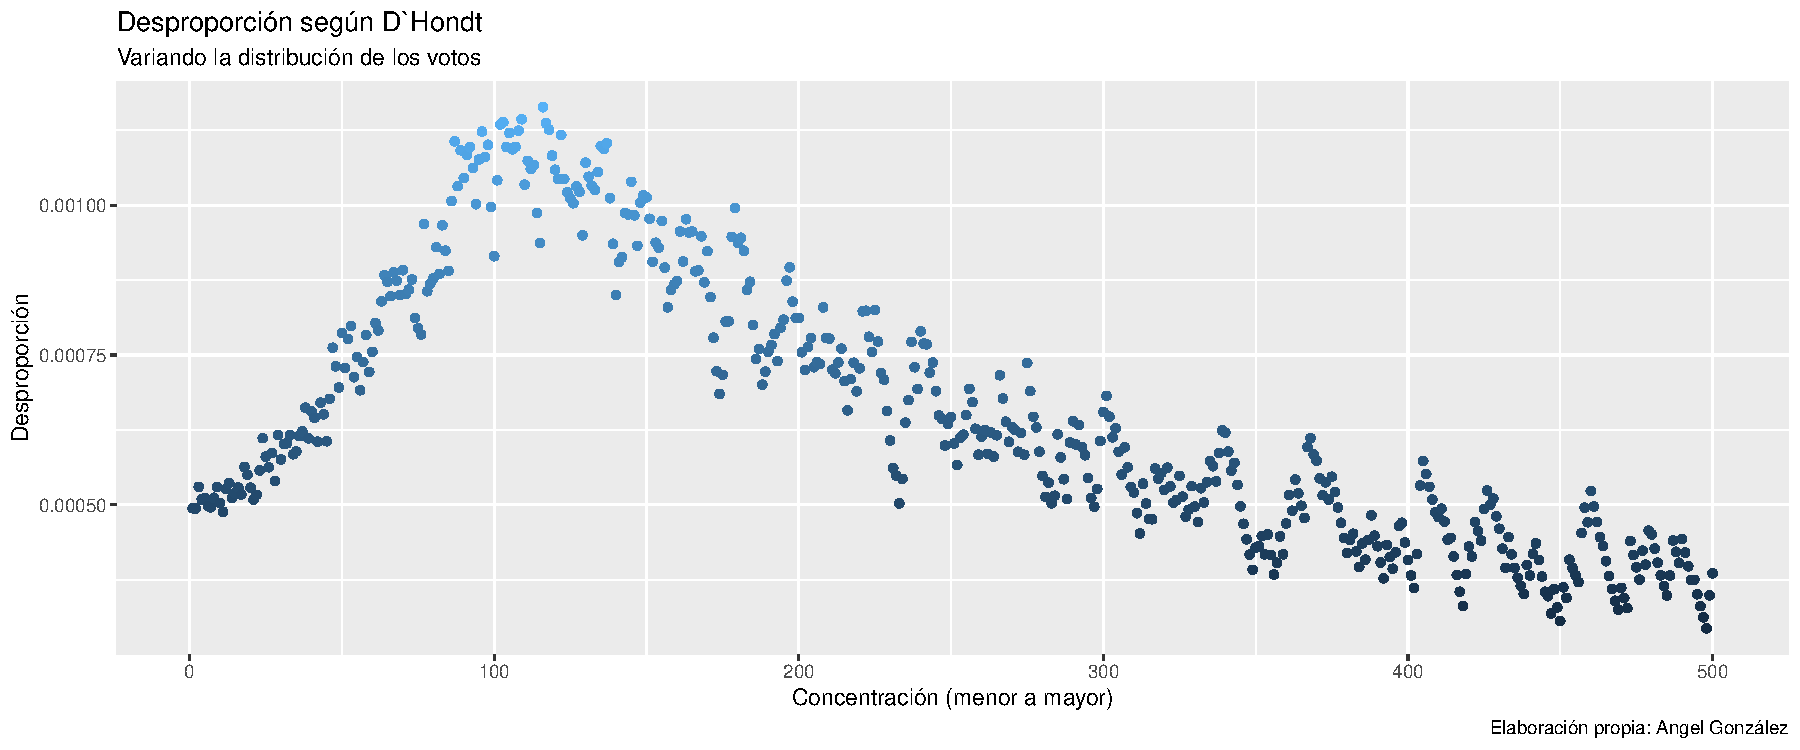
\includegraphics[width=0.95\linewidth]{figurasR/unnamed-chunk-11-1} \end{center}

\begin{center}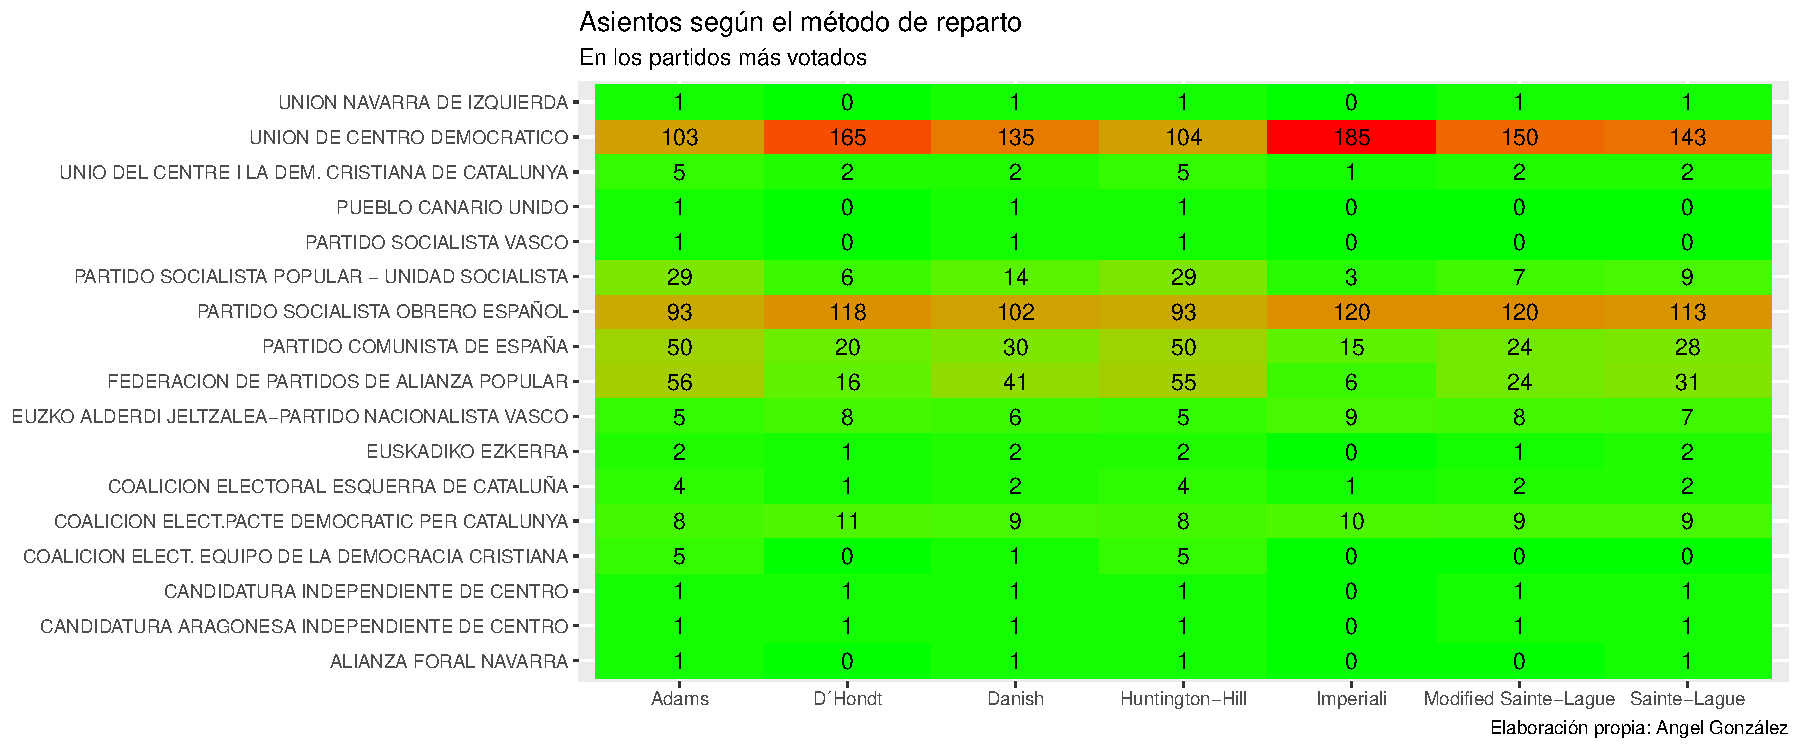
\includegraphics[width=0.95\linewidth]{figurasR/unnamed-chunk-11-2} \end{center}

\begin{center}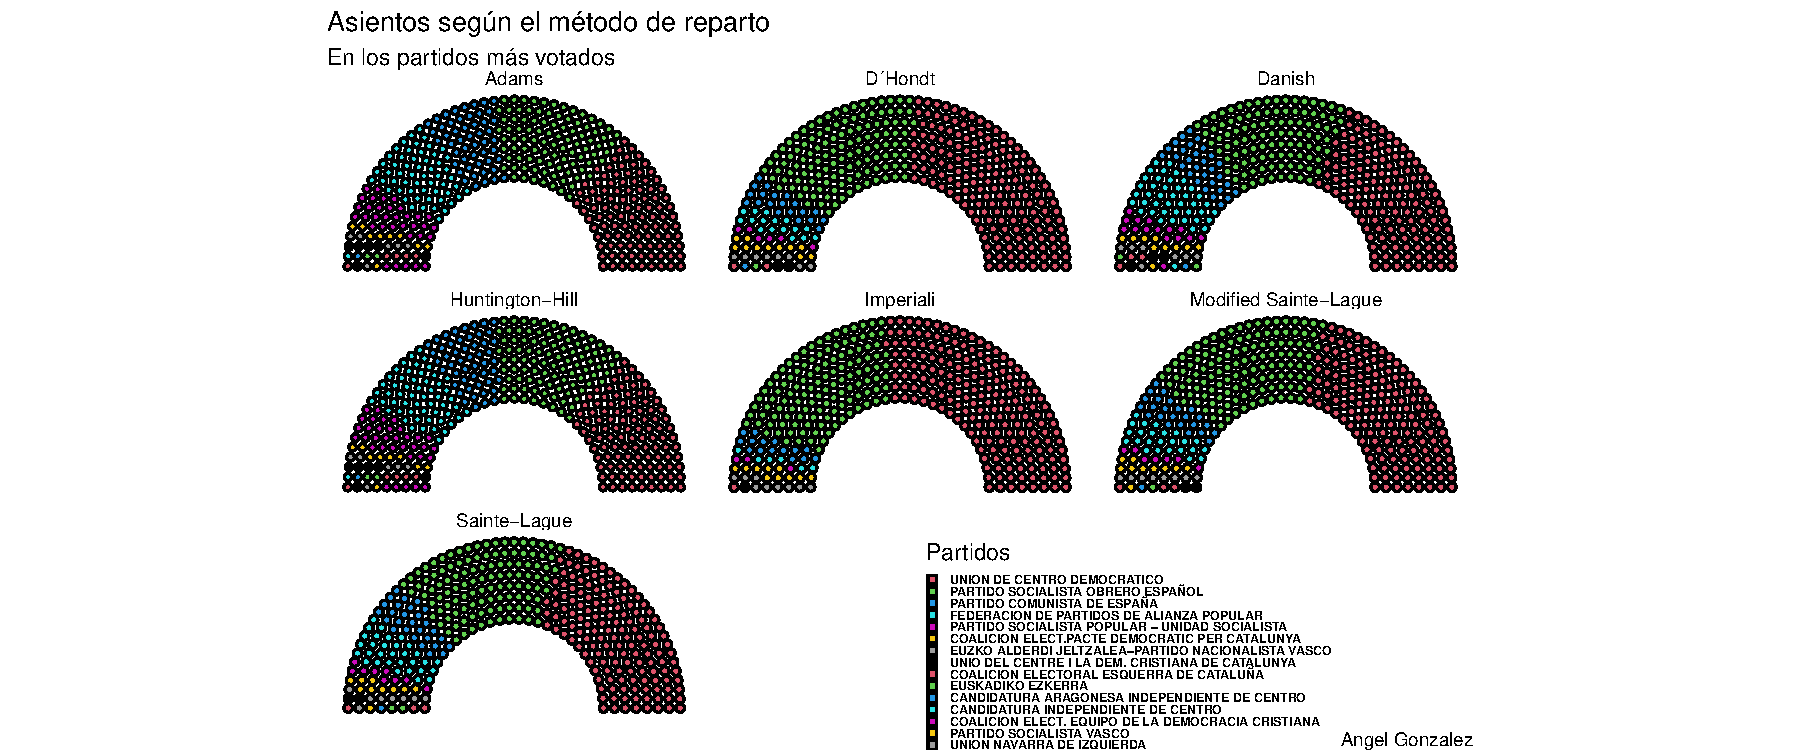
\includegraphics[width=0.95\linewidth]{figurasR/unnamed-chunk-11-3} \end{center}

En estas primeras elecciones de 1977 podemos observar que la fuerza más
votada en las elecciones es el partido \emph{Unión de Centro
democrático} seguido del \emph{PSOE}. Observamos que según el método
vigente en España, el método D´Hondt, el partido \emph{UCD}, que ganaría
las elecciones, tendría una gran diferencia de votos respecto a los
demás partidos, por lo que facilitaría la gobernabilidad.

Comparando entre métodos de reparto observamos que el que más escaños da
a los partidos grandes es el método imperiali, que beneficia mucho a los
partidos más votados y penaliza mucho en escaños a los partidos tanto
medianos como poco votados. El método actual en España también tiene un
comportamiento similar al imperiali aunque no tan acusado. En la otra
parte de la balanza encontramos al método Adams, el cual da muy pocos
escaños al partidos más votado y a los partidos medianos les beneficia.

En estas elecciones no se obtiene la mayoría absoluta en ningún método
excepto en el método imperiali, en los demás métodos el partido ganador
debería de aliarse con uno o dos partidos para obtener la mayoría
absoluta, los grandes perdedores en términos de escaños obtenidos son el
partido comunista y Alianza Popular, que podrían obtener hasta 10
escaños más de haber optado por otro método de reparto de votos.

\hypertarget{disproporcionalidad}{%
\subsubsection{Disproporcionalidad}\label{disproporcionalidad}}

\begin{center}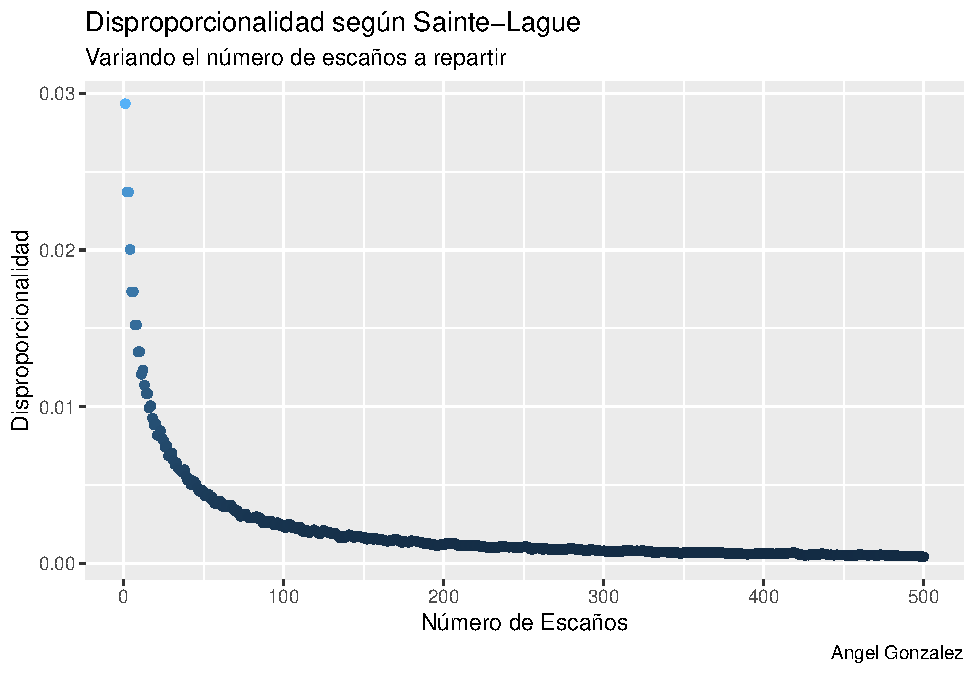
\includegraphics[width=0.95\linewidth]{figurasR/unnamed-chunk-12-1} \end{center}

\begin{center}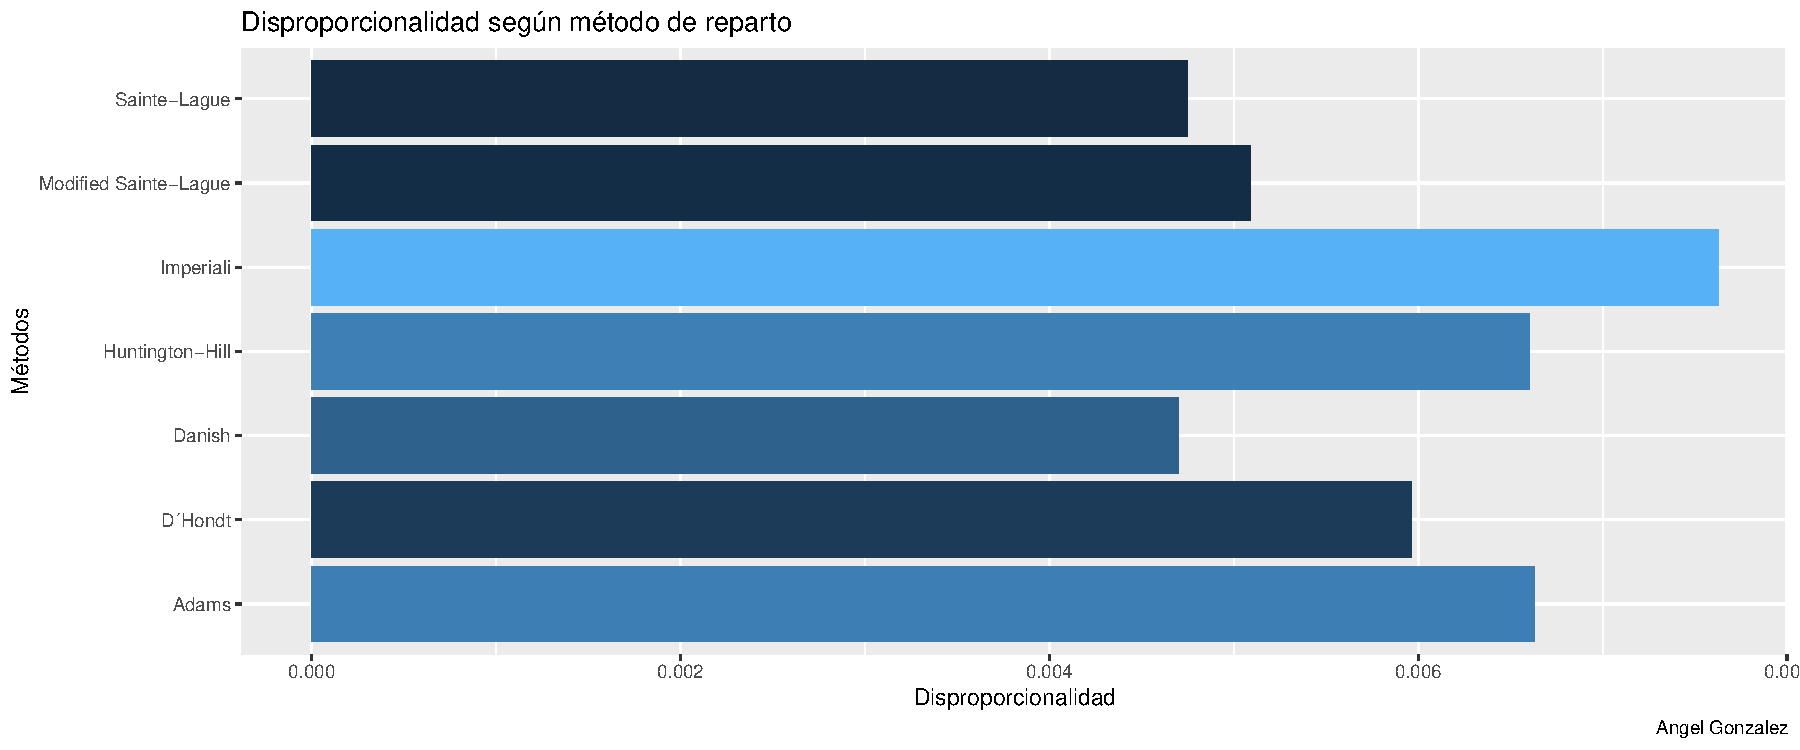
\includegraphics[width=0.95\linewidth]{figurasR/unnamed-chunk-12-2} \end{center}

En el presente gráfico, en el que se mide la desproporcionalidad por
comunidades, observamos que en general entre todos los métodos las
comunidades más desproporcionadas son las ciudades de Ceuta y Melilla,
resultado lógico en tanto que al repartirse un único escaño es el
partido más votado únicamente el que obtiene el escaño. Es común entre
todos los métodos que la comunidad de Madrid sea la comunidad más
proporcionada, esto es debido a que es la comunidad en la que se
reparten más asientos y también la más poblada, por lo que cuando se
reparten los asientos por provincias, al utilizar el método D´Hondt,
como hemos visto beneficia a los lugares con más población. En general
los métodos que presentan una menor diferencia de disproporcionalidad
entre las distintas comunidades autónomas son el método Danish y el
Saint-Lague, en cambio las que presentan una mayor diferencia entre
comunidades son el método Adams y el Huntington-Hill.

Si nos centramos en el gráfico de la disproporcionalidad media según el
método de reparto podemos observar que la menor disproporcionalidad se
encuentra en los métodos Danish y Sainte-Lague, mientras que las mayores
disproporcionalidades se encuentran en el método Imperiali y Adams.
Especial caso hacemos al método D´Hondt al ser el método utilizado
actualmente en España, observamos que ni es el mejor método ni tampoco
es de los peores, debido a ello sería conveniente cambiar el método de
reparto a otro mejor, que podría ser o bien el Sainte-Lague o el Danish.

\hypertarget{auxf1o-1979}{%
\section{Año 1979}\label{auxf1o-1979}}

\hypertarget{comparativa-entre-muxe9todos-1}{%
\subsection{Comparativa entre
métodos}\label{comparativa-entre-muxe9todos-1}}

\hypertarget{votos-obtenidos-1}{%
\subsubsection{Votos obtenidos}\label{votos-obtenidos-1}}

\begin{center}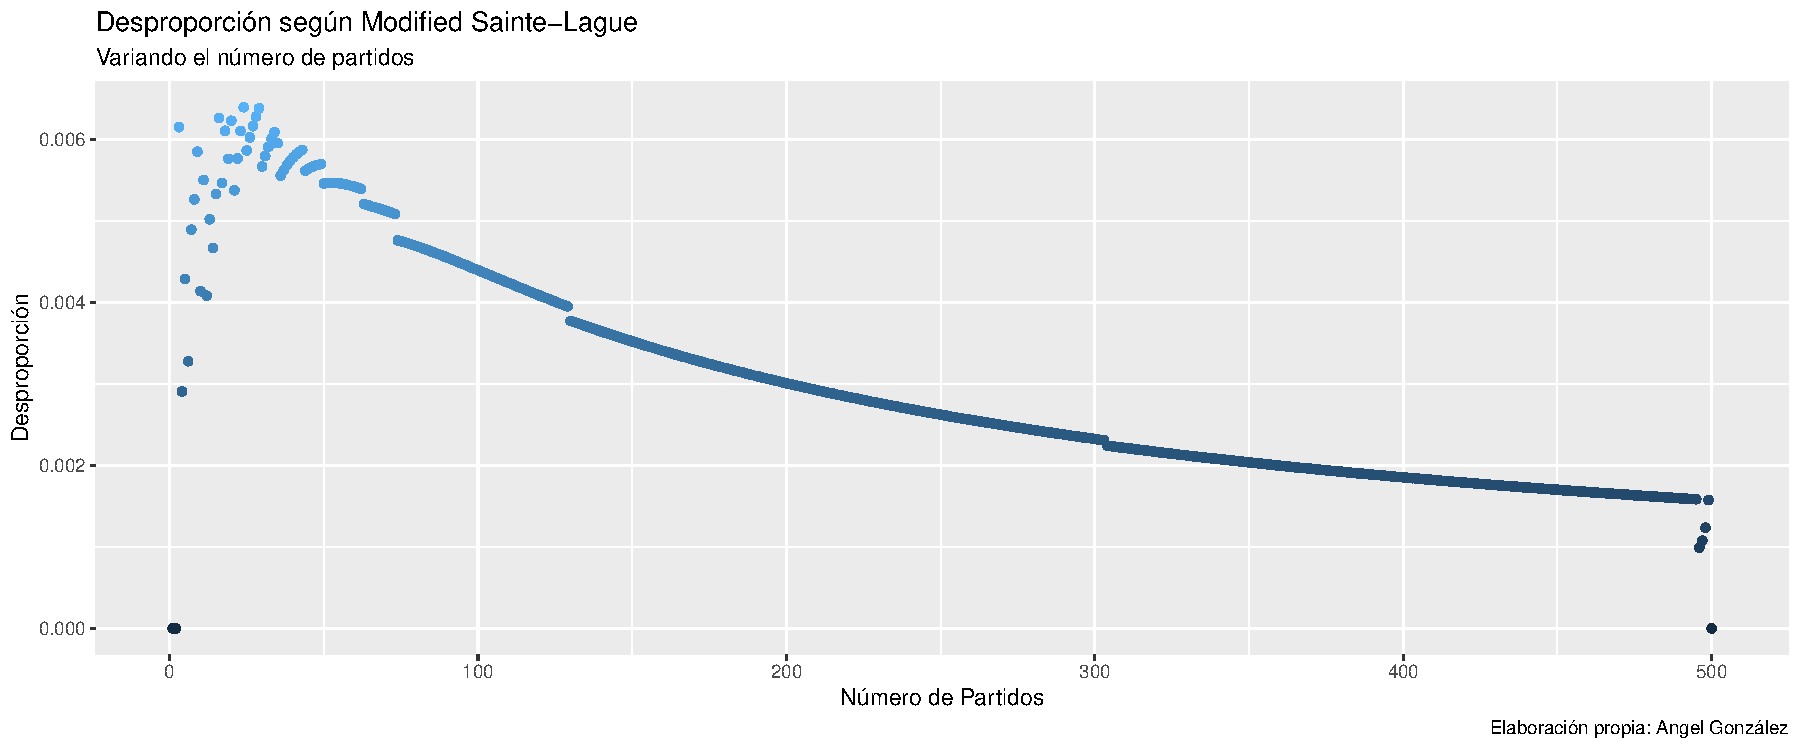
\includegraphics[width=0.95\linewidth]{figurasR/unnamed-chunk-20-1} \end{center}

\begin{center}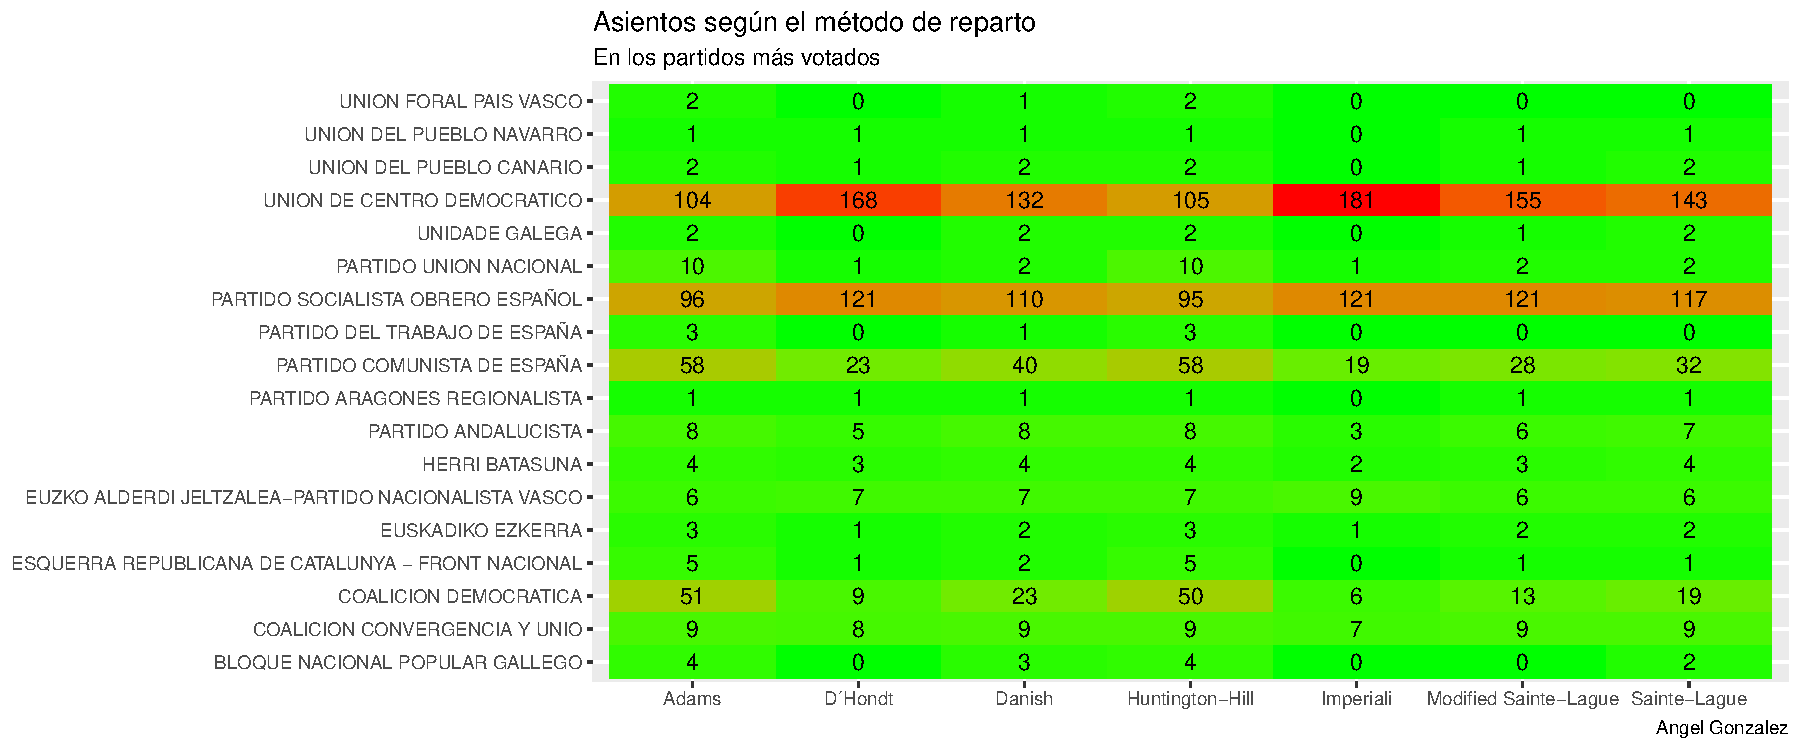
\includegraphics[width=0.95\linewidth]{figurasR/unnamed-chunk-20-2} \end{center}

\begin{center}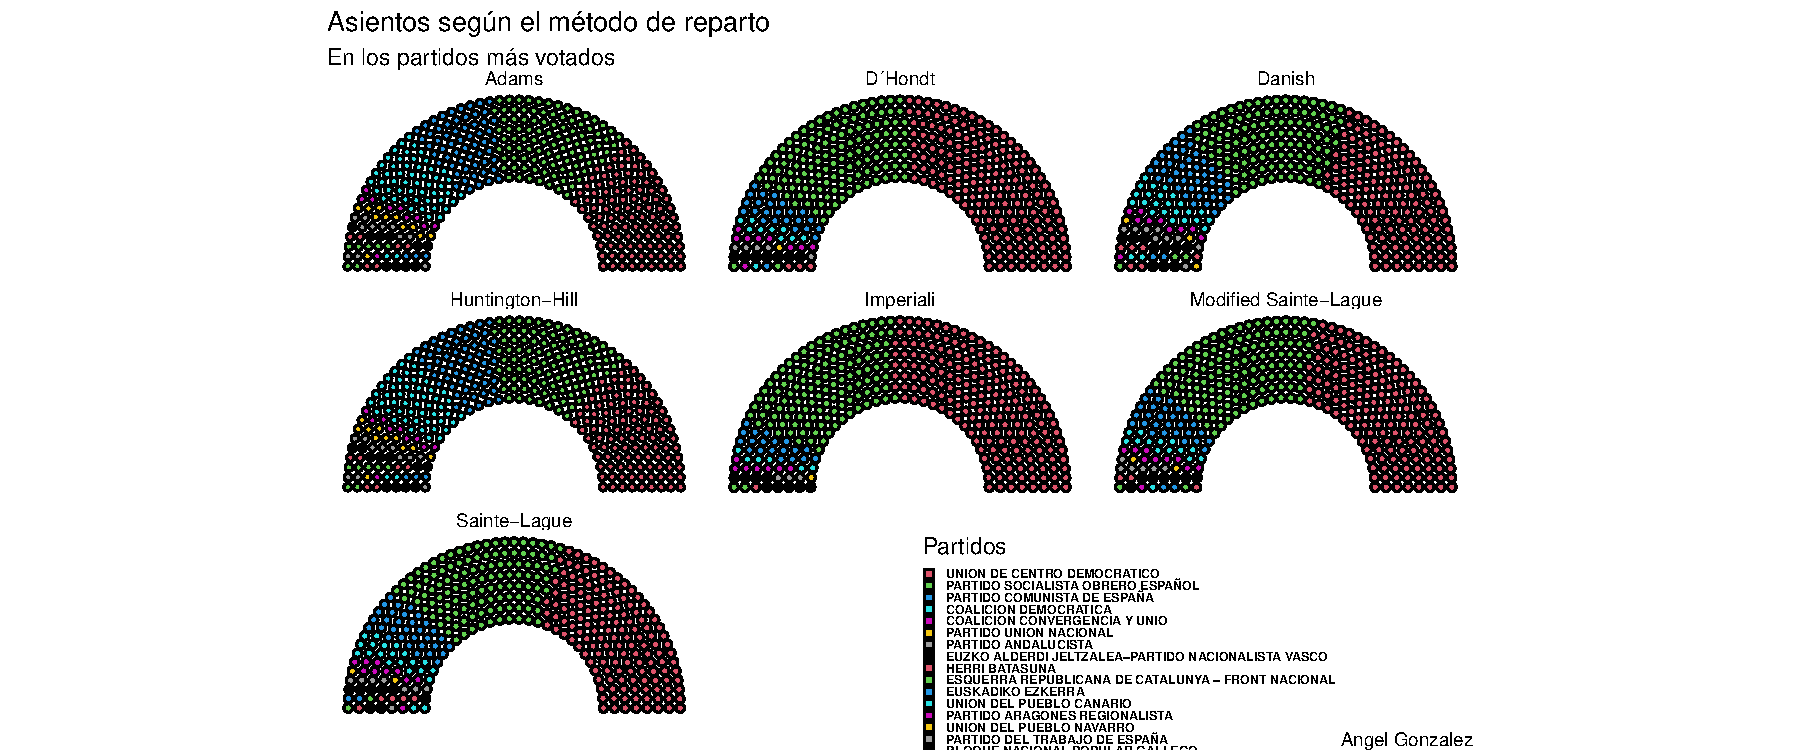
\includegraphics[width=0.95\linewidth]{figurasR/unnamed-chunk-20-3} \end{center}

En estas elecciones de 1979 el partido más votado fué \emph{UCD} seguido
del \emph{PSOE}, según los distintos métodos de reparto únicamente en el
método Imperiali UCD conseguiría la mayoría absoluta, en todos los demás
métodos de reparto no se alcanza la mayoría absoluta, los partidos más
castigados por utilizar el método D´Hondt son el partido comunista y
coalición Democrática, que podrían hasta doblar el número de asientos
obtenidos dependiendo del método de reparto que se haya realizado. En
estas elecciones podemos decir que hay dos grandes partidos y dos
medianos, UCD y el PSOE son los más grandes y el partido comunista y
coalición democrática son los partidos medianos, después ya se
encuentran todos los demás.

\hypertarget{disproporcionalidad-1}{%
\subsubsection{Disproporcionalidad}\label{disproporcionalidad-1}}

\begin{center}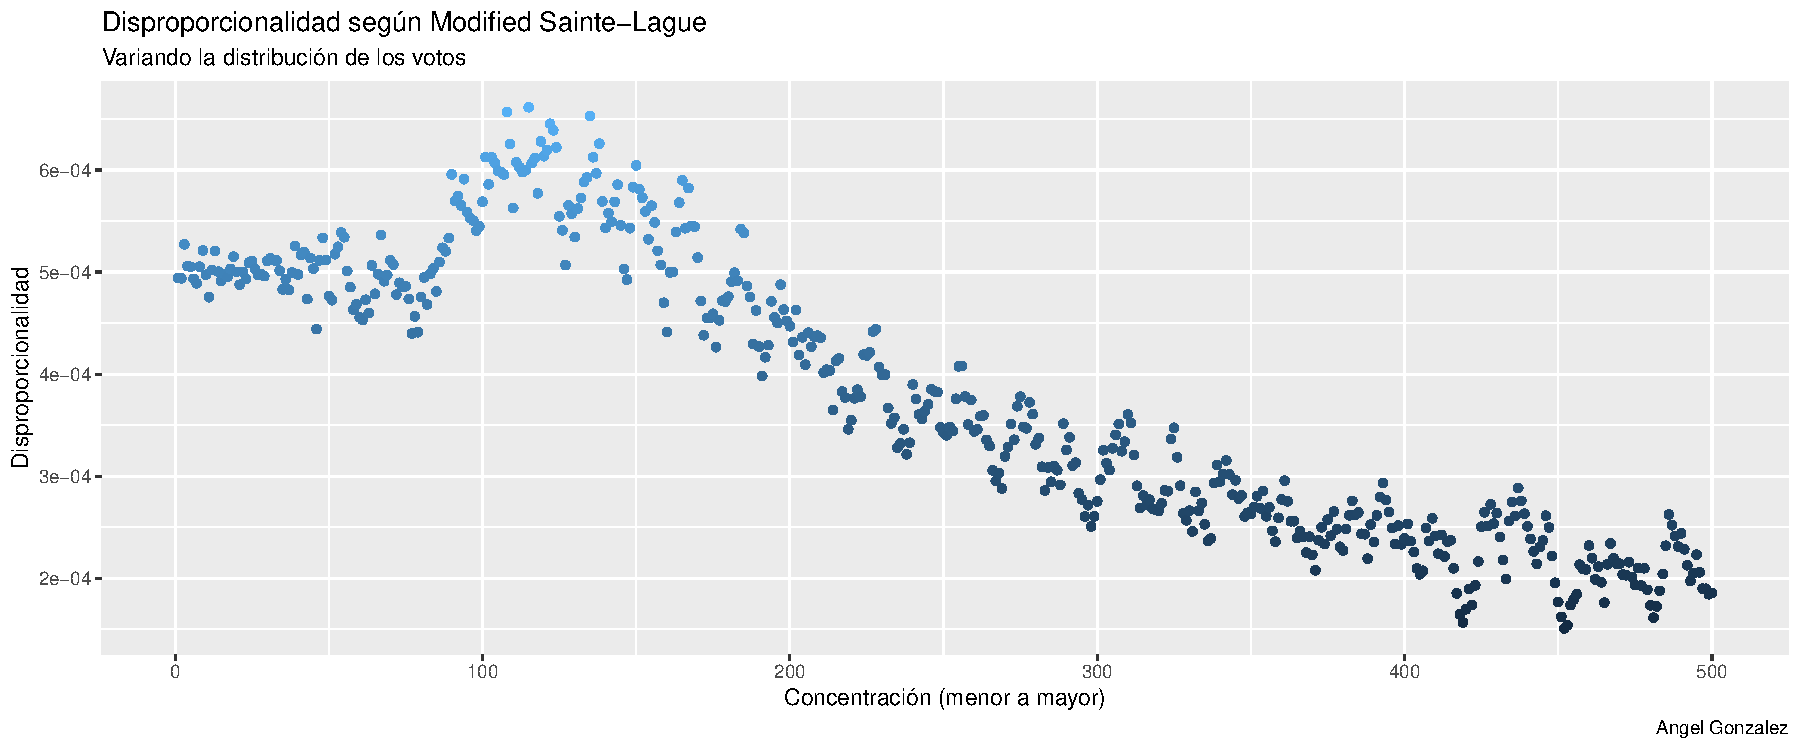
\includegraphics[width=0.95\linewidth]{figurasR/unnamed-chunk-21-1} \end{center}

\begin{center}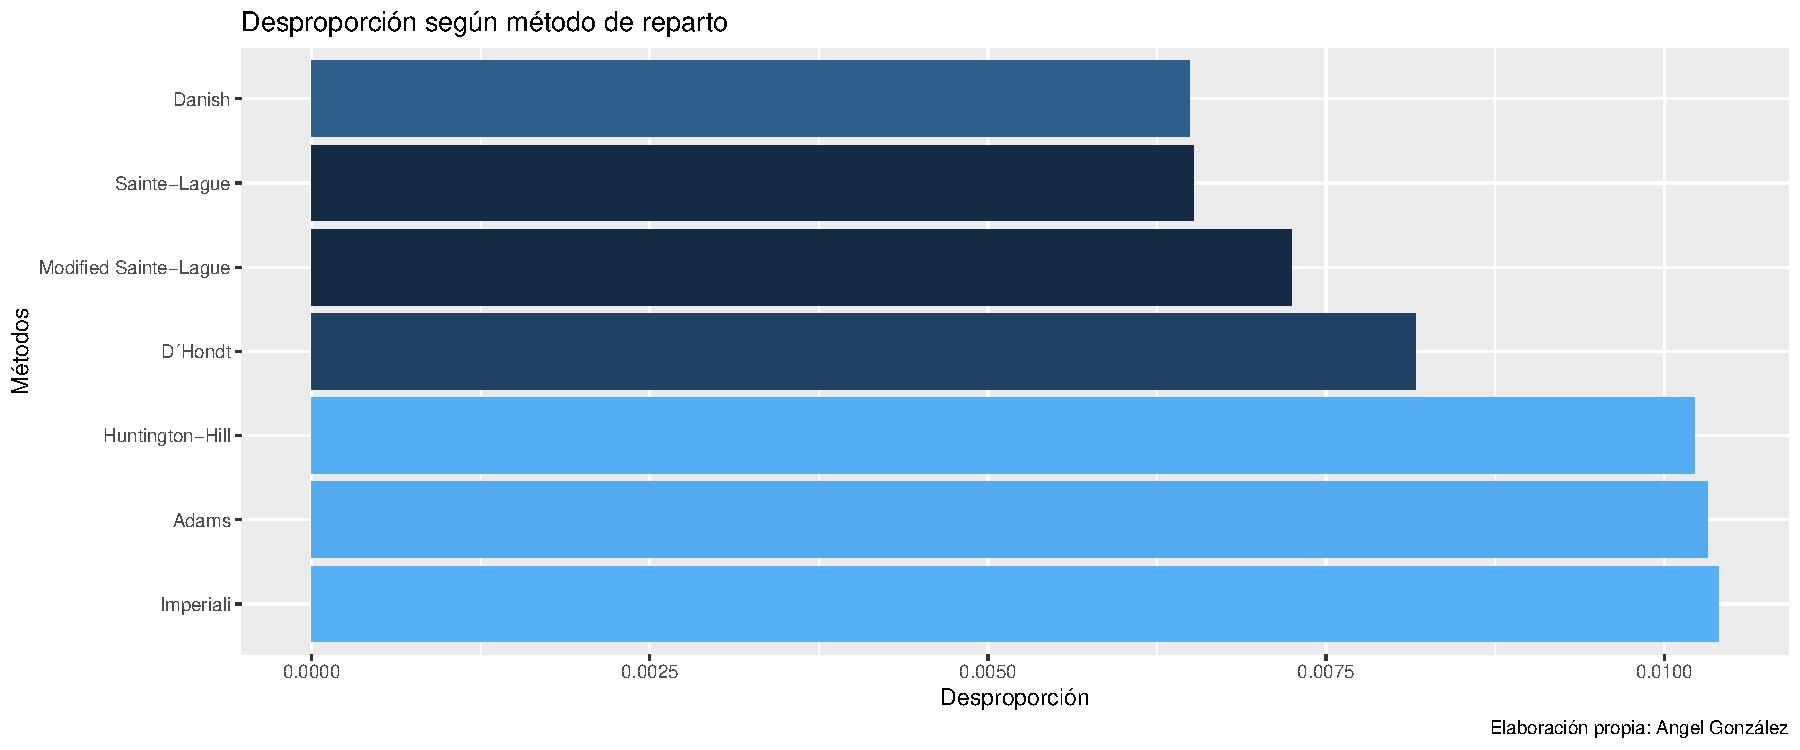
\includegraphics[width=0.95\linewidth]{figurasR/unnamed-chunk-21-2} \end{center}

En el presente gráfico vemos como respecto a las anteriores elecciones
hay una mayor diferencia de disproporcionalidad entre comunidades,
siguen teniendo las ciudades de Ceuta y Melilla la mayor
disproporcionalidad y la comunidad de Madrid la menor
disproporcionalidad.

Según la disproporcionalidad media los peores métodos de reparto se
pueden agrupar en tres, el método Imperiali, el Huntington-Hill, y el
Adams, y los mejores métodos de reparto en dos métodos, el Danish y el
Sainte-Lague. En el caso del método D´Hondt se encuentra en un término
medio, por lo que sería conveniente cambiar el método de reparto a uno
más proporcional, que puede ser el Danish o el Sainte-Lague.

\hypertarget{auxf1o-1982}{%
\section{Año 1982}\label{auxf1o-1982}}

\hypertarget{comparativa-entre-muxe9todos-2}{%
\subsection{Comparativa entre
métodos}\label{comparativa-entre-muxe9todos-2}}

\hypertarget{votos-obtenidos-2}{%
\subsubsection{Votos obtenidos}\label{votos-obtenidos-2}}

\begin{center}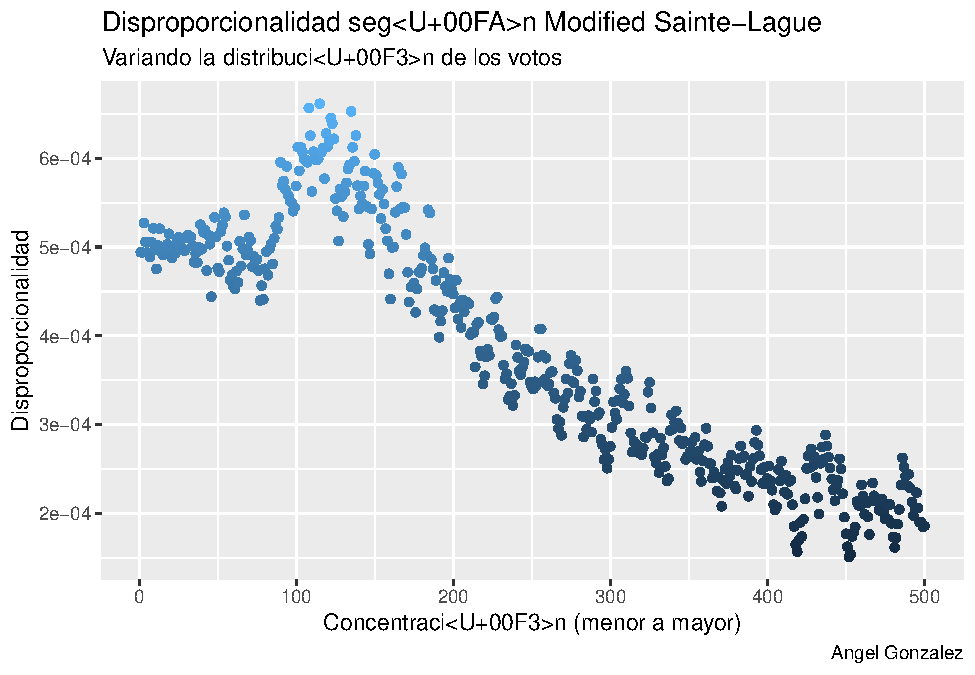
\includegraphics[width=0.95\linewidth]{figurasR/unnamed-chunk-29-1} \end{center}

\begin{center}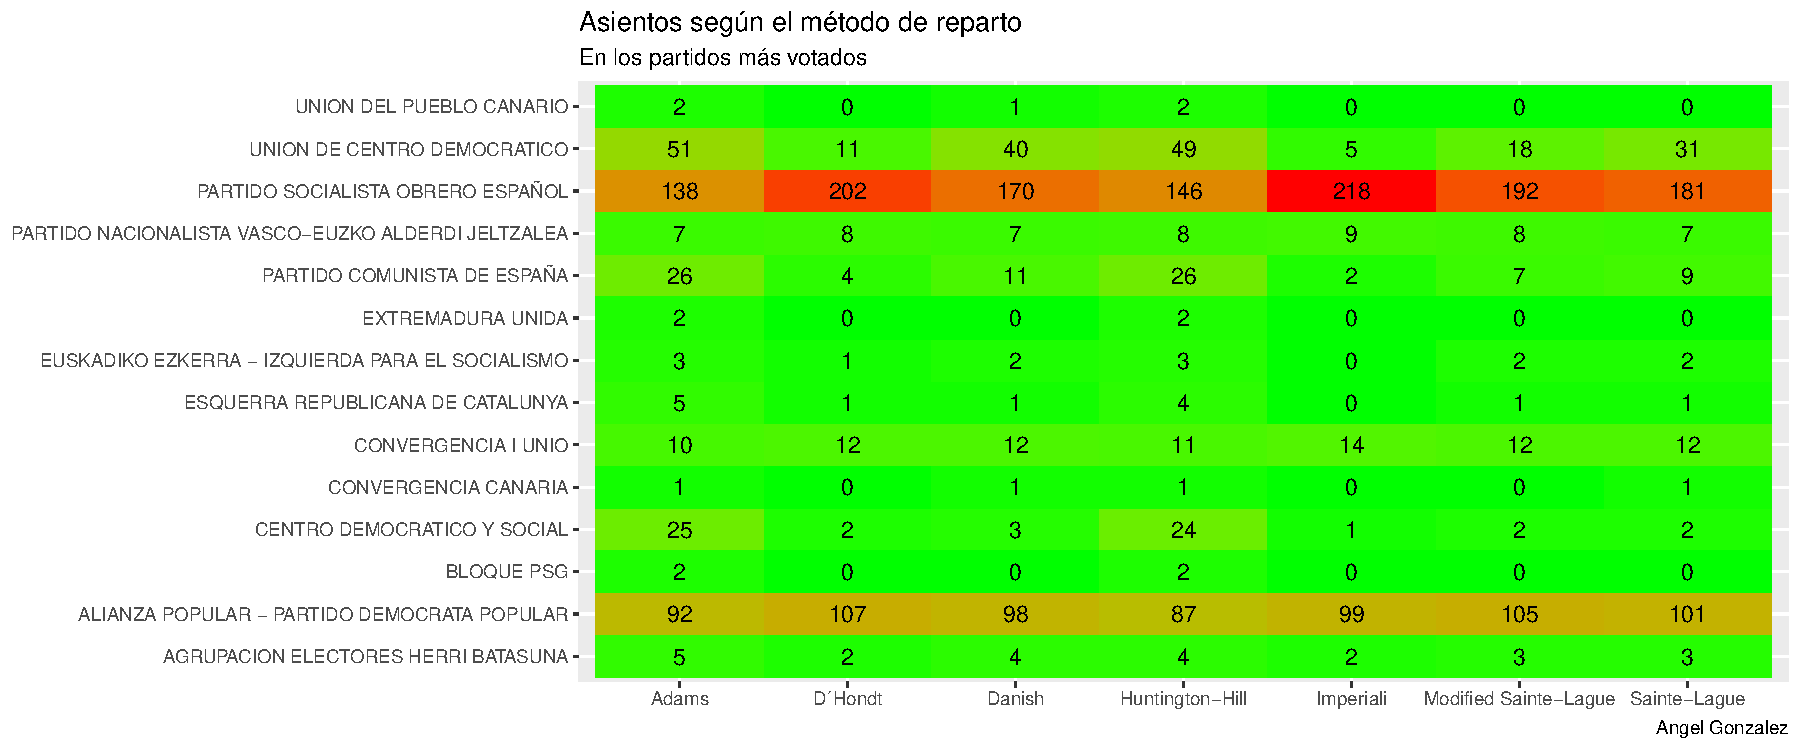
\includegraphics[width=0.95\linewidth]{figurasR/unnamed-chunk-29-2} \end{center}

\begin{center}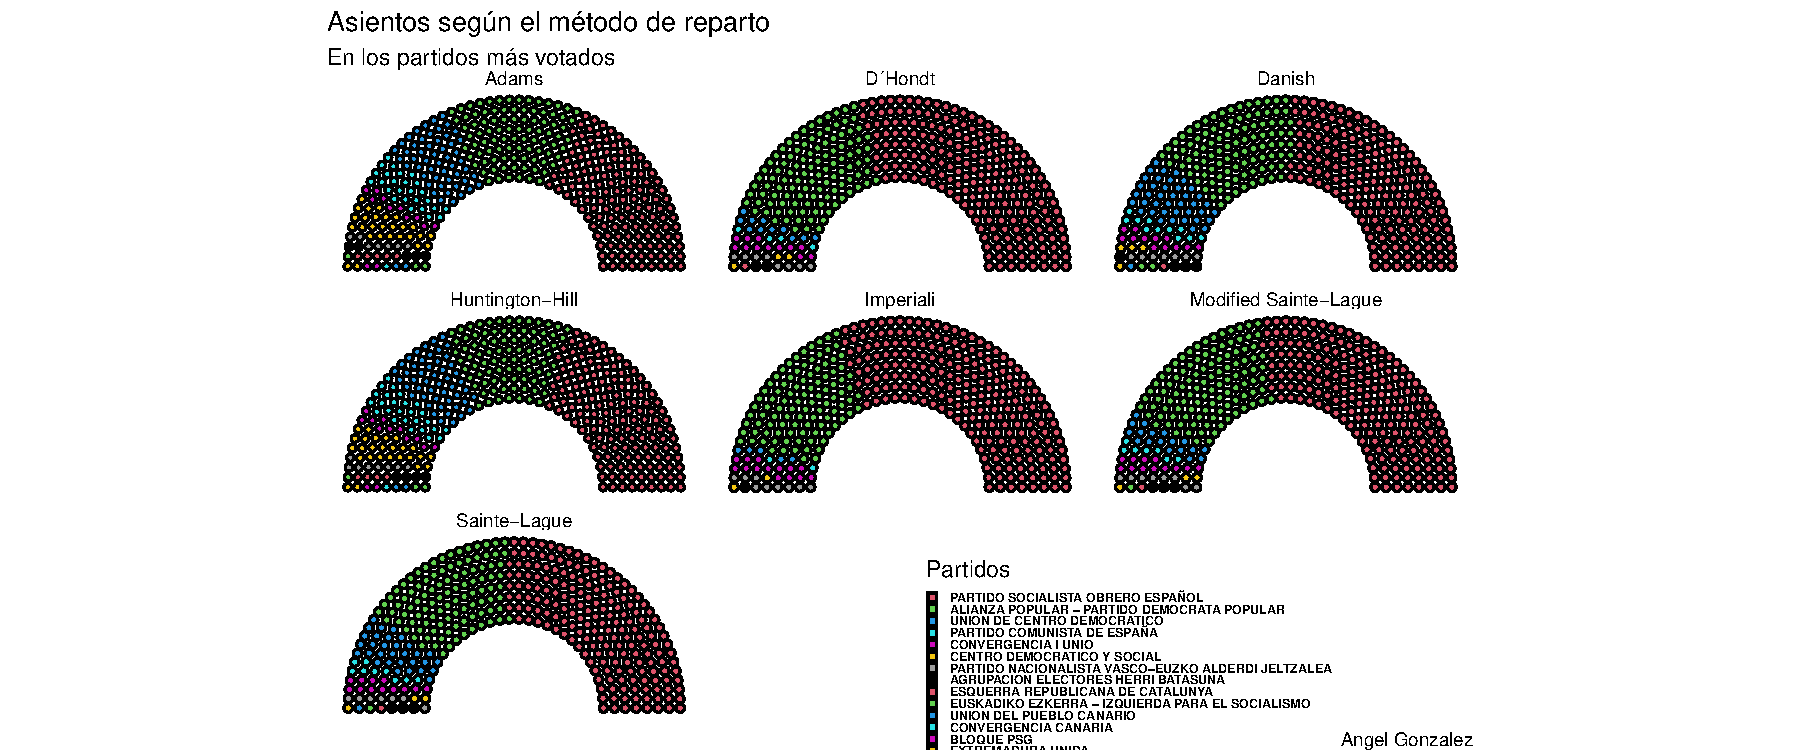
\includegraphics[width=0.95\linewidth]{figurasR/unnamed-chunk-29-3} \end{center}

En estas elecciones de 1982 el partido más votado es el \emph{PSOE} el
cual según la mayoría de los métodos de reparto, incluido el método
D´Hondt, alcanza la mayoría absoluta. Son unas elecciones en los que el
voto se concentra únicamente en dos partidos, que son el PSOE y Alianza
Popular, pero con una gran diferencia de asientos entre ellos, donde el
PSOE casi dobla en escaños a Alianza Popular. El partido menos
beneficiado en este año es UCD, que según el método D´Hondt obtendría 11
escaños mientras que si se optase por otro método más proporcional como
puede ser el método Danish o bien el Sainte-Lague podría multiplicar por
3 o 4 sus escaños.

\hypertarget{disproporcionalidad-2}{%
\subsubsection{Disproporcionalidad}\label{disproporcionalidad-2}}

\begin{center}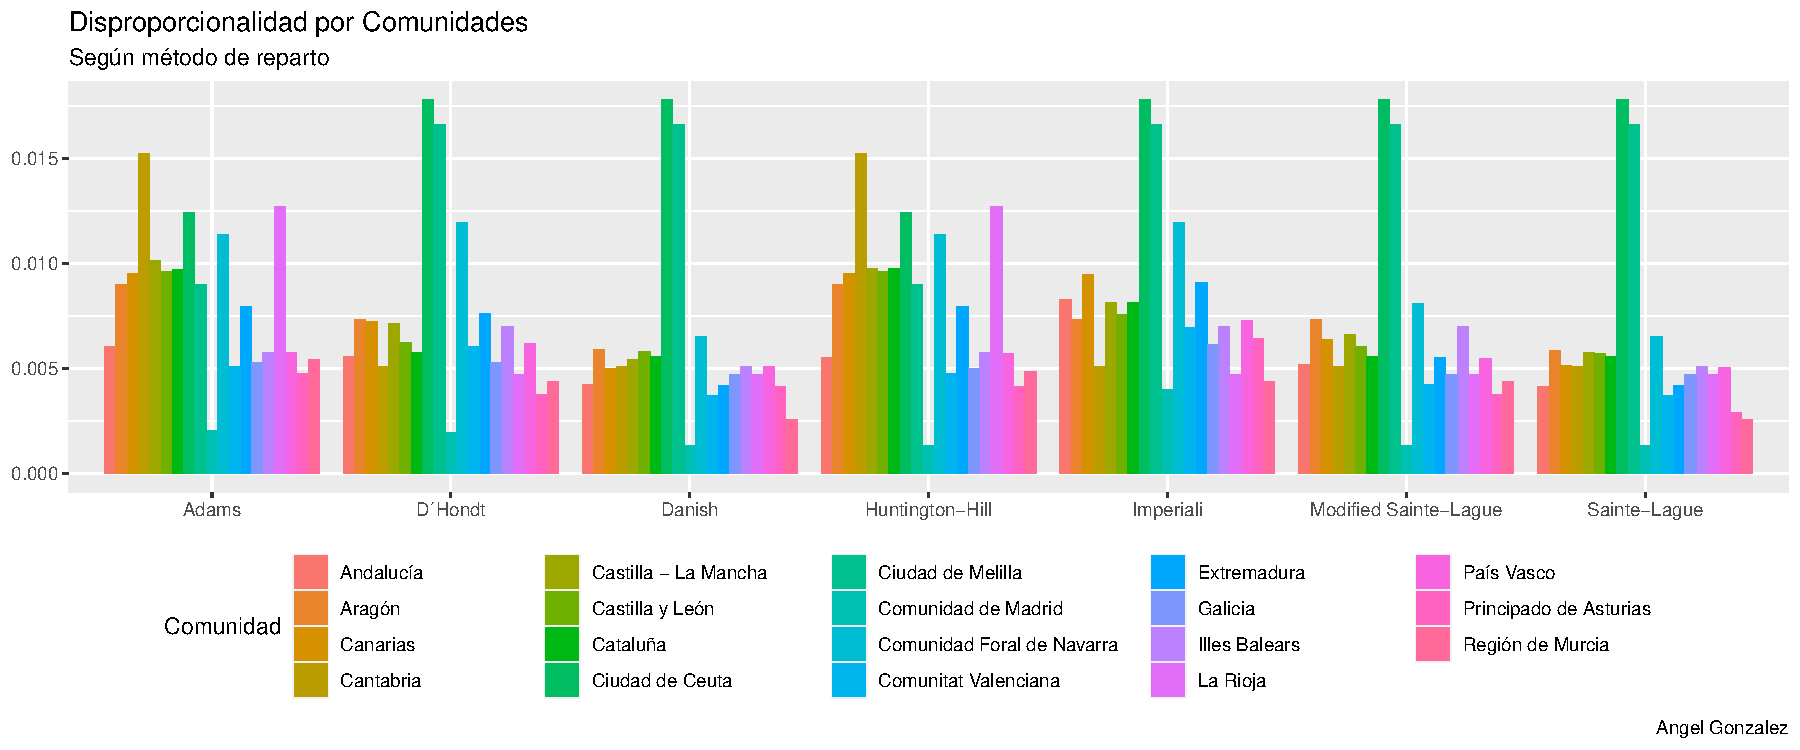
\includegraphics[width=0.95\linewidth]{figurasR/unnamed-chunk-30-1} \end{center}

\begin{center}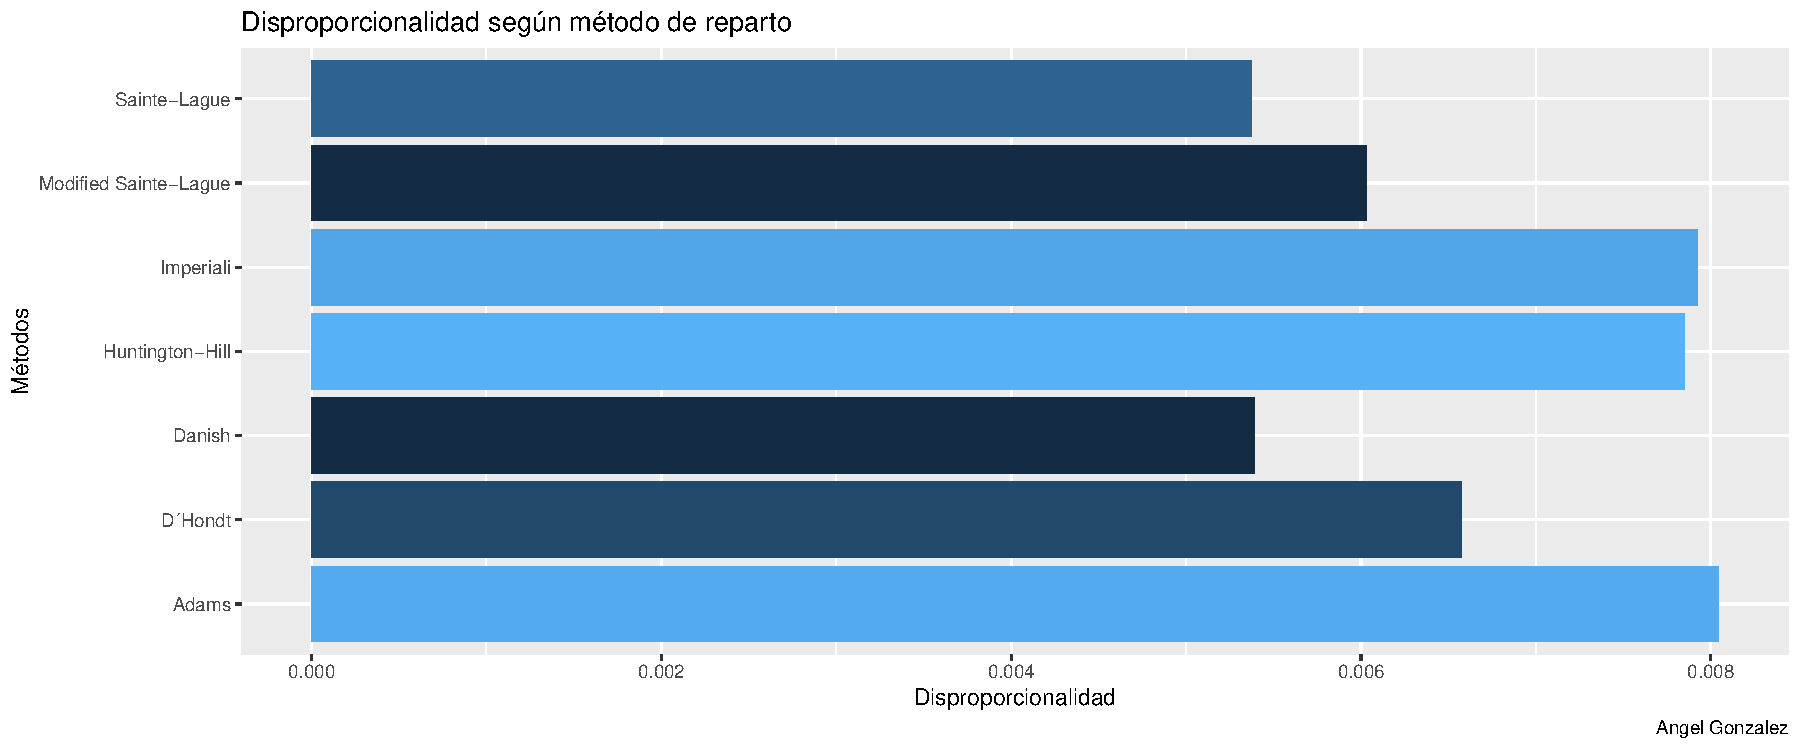
\includegraphics[width=0.95\linewidth]{figurasR/unnamed-chunk-30-2} \end{center}

Según la gráfica de disproporcionalidad por comunidades es un año en el
que generalmente no hay mucha diferencia de disproporcionalidad entre
ellas, este año las comunidades más desproporcionadas son la comunidad
Foral de Navarra y Cantabria mientras que las comunidades más
proporcionadas son la comunidad de Madrid y la región de Murcia.

Según la disproporción media, se reconocen tres grupos distintos, un
grupo muy disproporcionado, con el método Imperiali como el más
disproporcionado, otro grupo medio en donde se encontraría el método
D´Hondt y un último grupo el cual sería el más proporcionado en el que
se encontraría el método Danish y el Saint-Lague.

\hypertarget{auxf1o-1986}{%
\section{Año 1986}\label{auxf1o-1986}}

\hypertarget{comparativa-entre-muxe9todos-3}{%
\subsection{Comparativa entre
métodos}\label{comparativa-entre-muxe9todos-3}}

\hypertarget{votos-obtenidos-3}{%
\subsubsection{Votos obtenidos}\label{votos-obtenidos-3}}

\begin{center}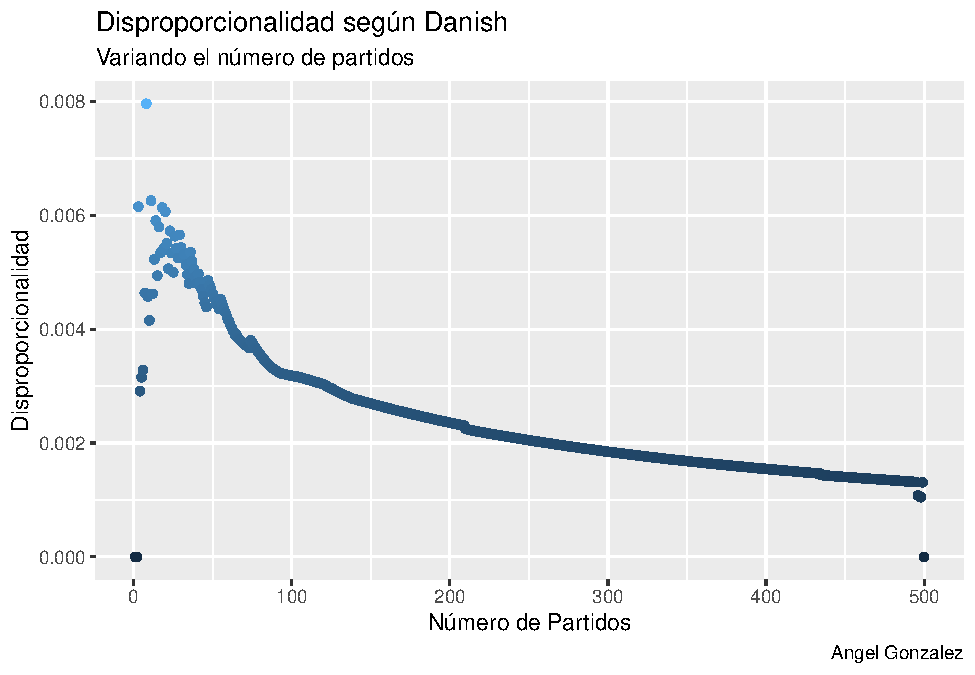
\includegraphics[width=0.95\linewidth]{figurasR/unnamed-chunk-38-1} \end{center}

\begin{center}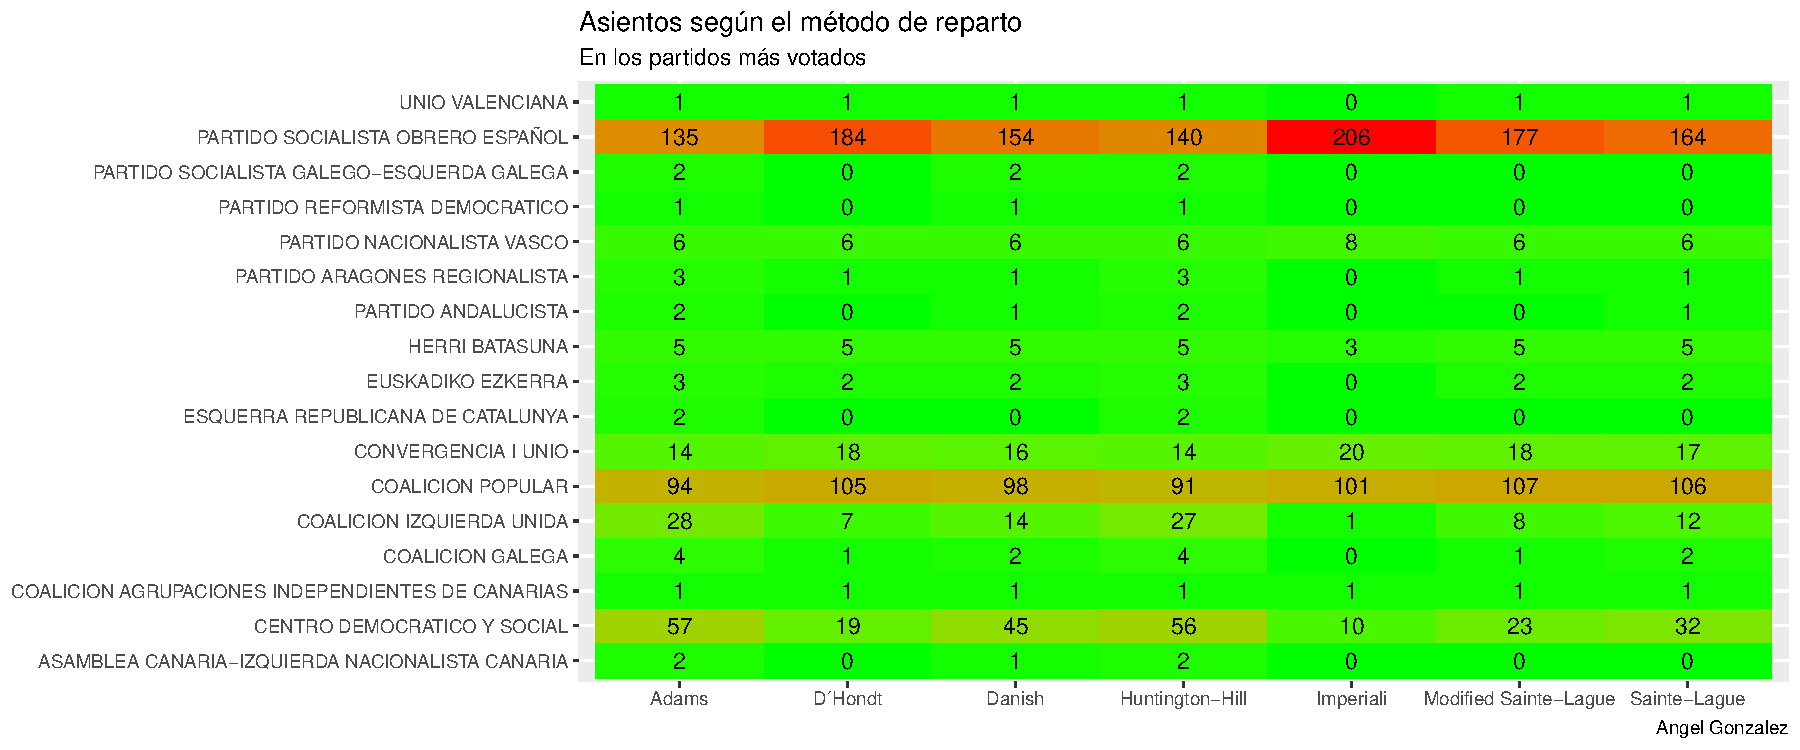
\includegraphics[width=0.95\linewidth]{figurasR/unnamed-chunk-38-2} \end{center}

\begin{center}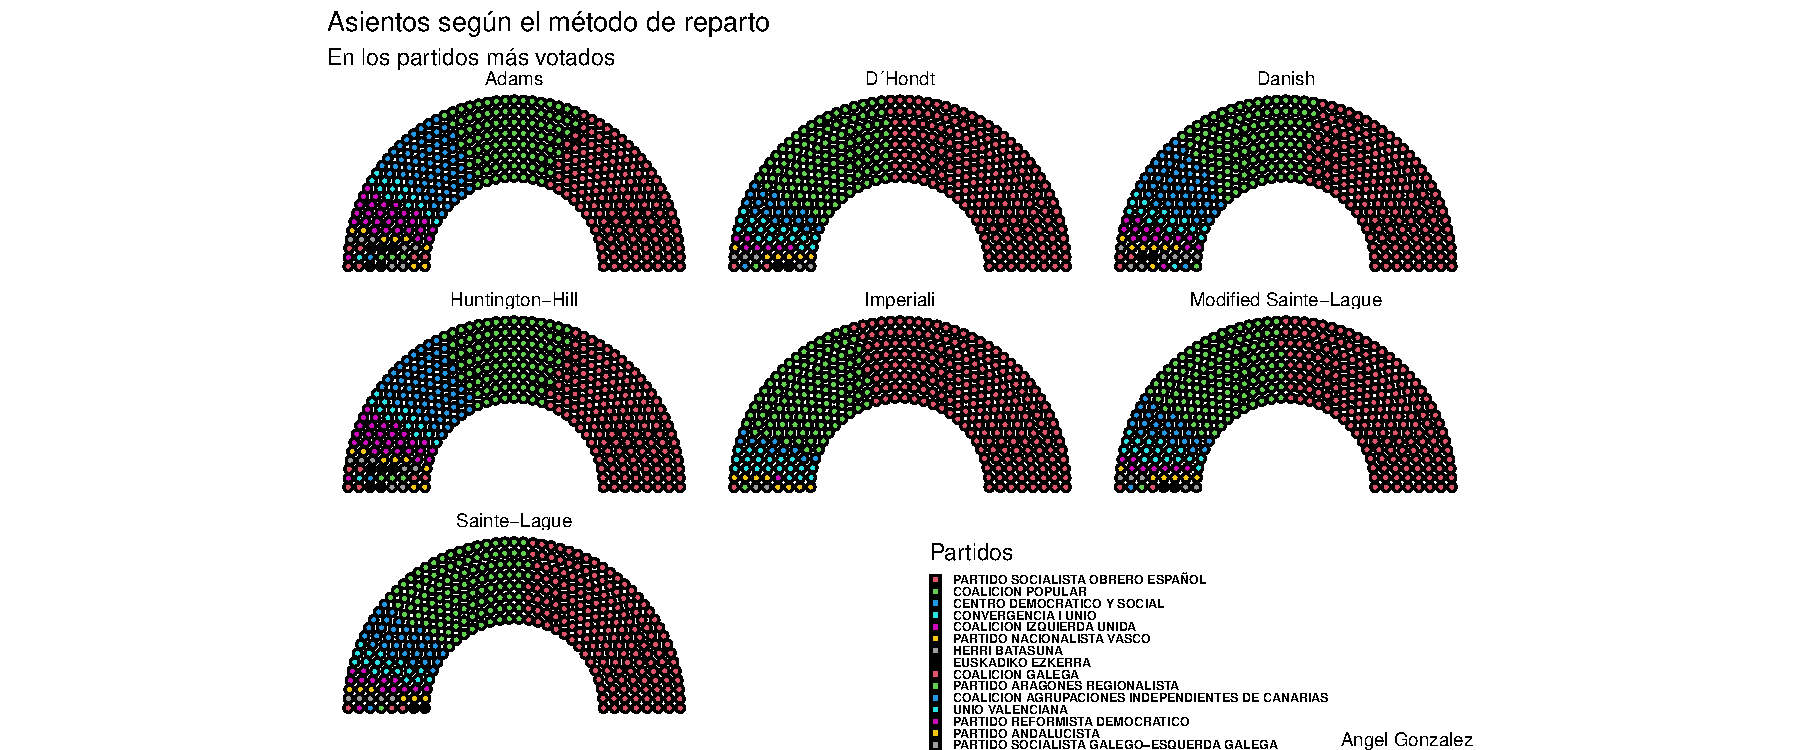
\includegraphics[width=0.95\linewidth]{figurasR/unnamed-chunk-38-3} \end{center}

En estas elecciones de 1986 el partido más votado fué el \emph{PSOE},
tal y como sucedió en las anteriores elecciones, son también unas
elecciones en donde hay únicamente dos partidos mayoritarios,
\emph{PSOE} y \emph{Coalición Popular}, ocurre en estas elecciones el
mismo escenario que en las anteriores elecciones, en donde el primer
partido casi dobla en escaños al segundo partido, aunque en este caso ya
se puede apreciar que la diferencia se va reduciendo entre los dos
grandes partidos, en general el PSOE alcanza la mayoría absoluta pero en
este año si utilizásemos los métodos más proporcionados es interesante
observar como perdería la mayoría absoluta tanto utilizando el método
Danish como el Sainte-Lague. Este año también reconocemos un partido que
podría decirse de nivel de votos medio que queda muy dañado por el
método de reparto D´Hondt, es el partido \emph{Centro Democrático y
Social}, el cual de utilizar los métodos más proporcionados podría hasta
duplicar sus escaños en el caso de optar por el método Danish.

\hypertarget{disproporcionalidad-3}{%
\subsubsection{Disproporcionalidad}\label{disproporcionalidad-3}}

\begin{center}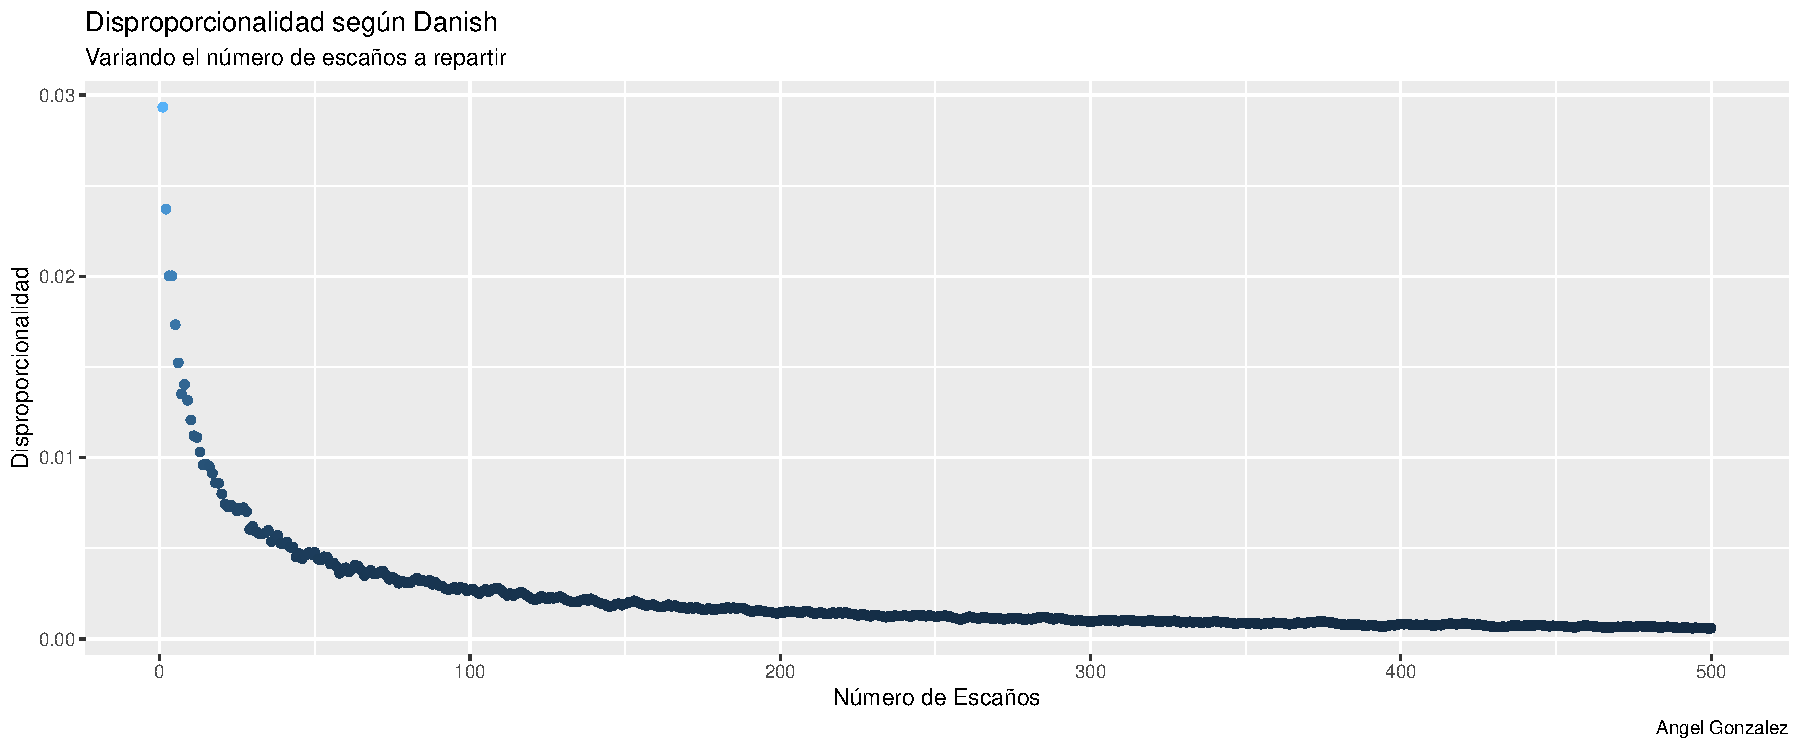
\includegraphics[width=0.95\linewidth]{figurasR/unnamed-chunk-39-1} \end{center}

\begin{center}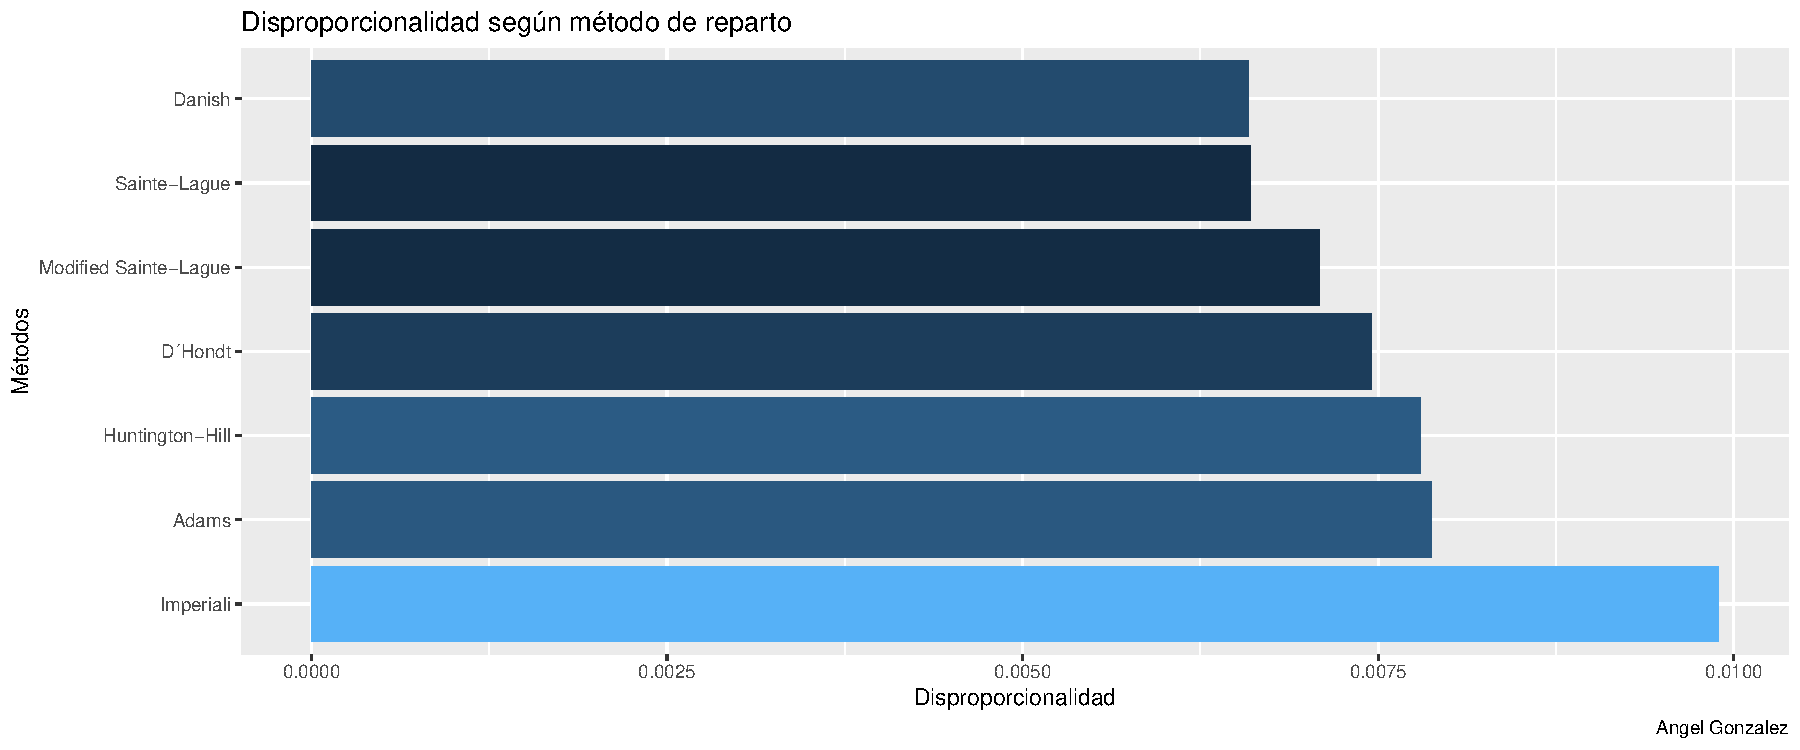
\includegraphics[width=0.95\linewidth]{figurasR/unnamed-chunk-39-2} \end{center}

Este año en el caso de la disproporción por comunidades podemos observar
que aumenta la diferencia respecto a las pasadas elecciones, una de las
comunidades más proporcionadas es la comunidad de Asturias mientras que
Aragón pasa a ser ahora una de las que más desproporción presenta. En
los extremos no hay novedades, Madrid sigue siendo la más proporcionada
y las ciudades de Ceuta y Melilla las que menos proporcionadas resultan.

Según el método de reparto este año el método Imperiali es el más
disproporcionado con diferencia, los demás métodos se podrían en un
mismo grupo, en donde el método más proporcionado este año es el método
Danish.

\hypertarget{auxf1o-1989}{%
\section{Año 1989}\label{auxf1o-1989}}

\hypertarget{comparativa-entre-muxe9todos-4}{%
\subsection{Comparativa entre
métodos}\label{comparativa-entre-muxe9todos-4}}

\hypertarget{votos-obtenidos-4}{%
\subsubsection{Votos obtenidos}\label{votos-obtenidos-4}}

\begin{center}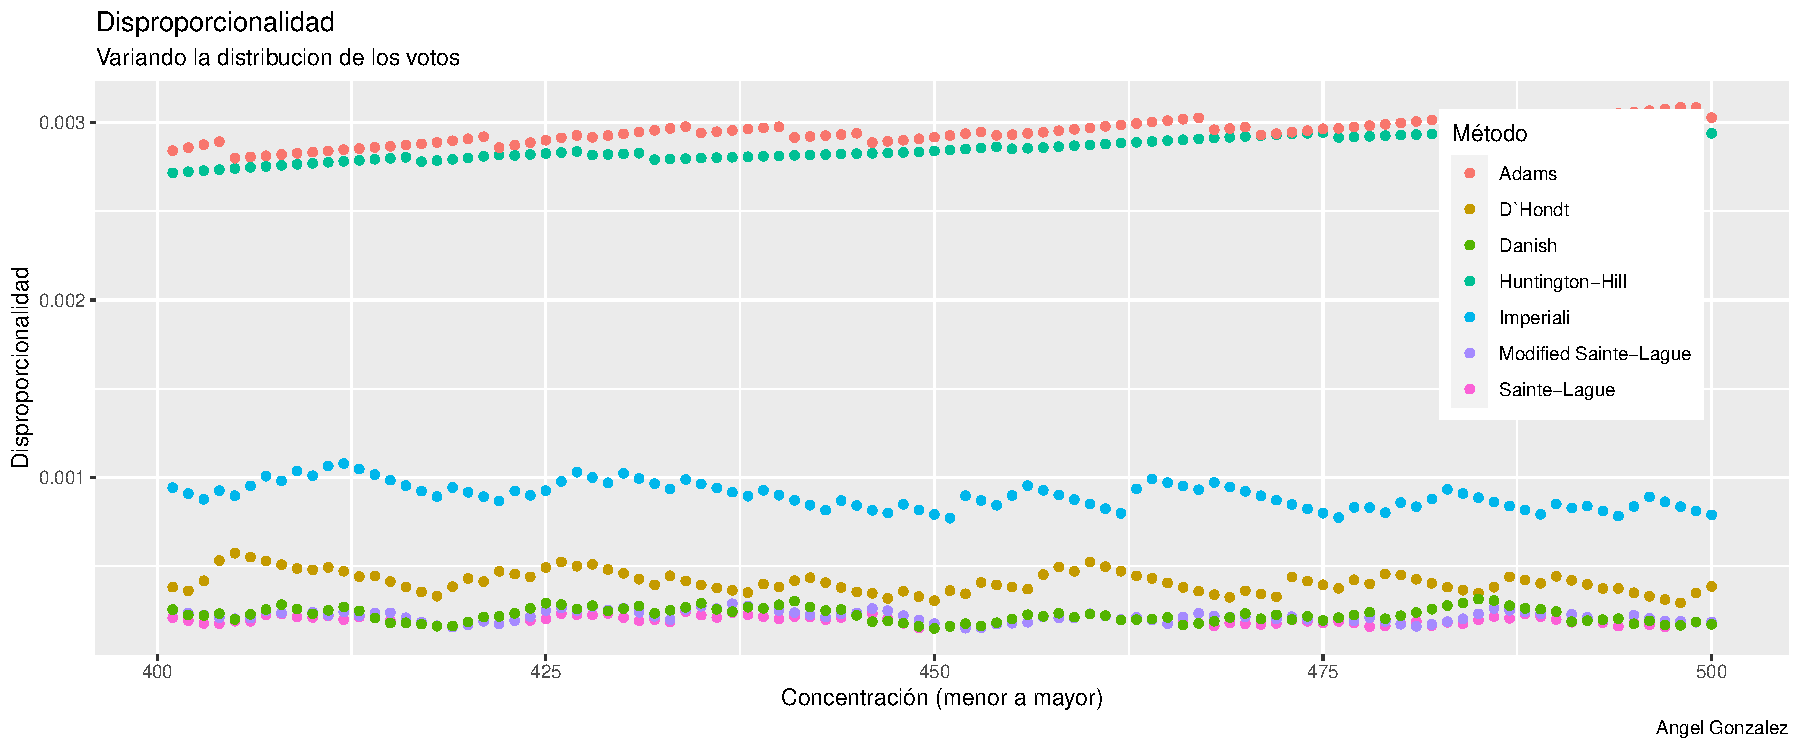
\includegraphics[width=0.95\linewidth]{figurasR/unnamed-chunk-47-1} \end{center}

\begin{center}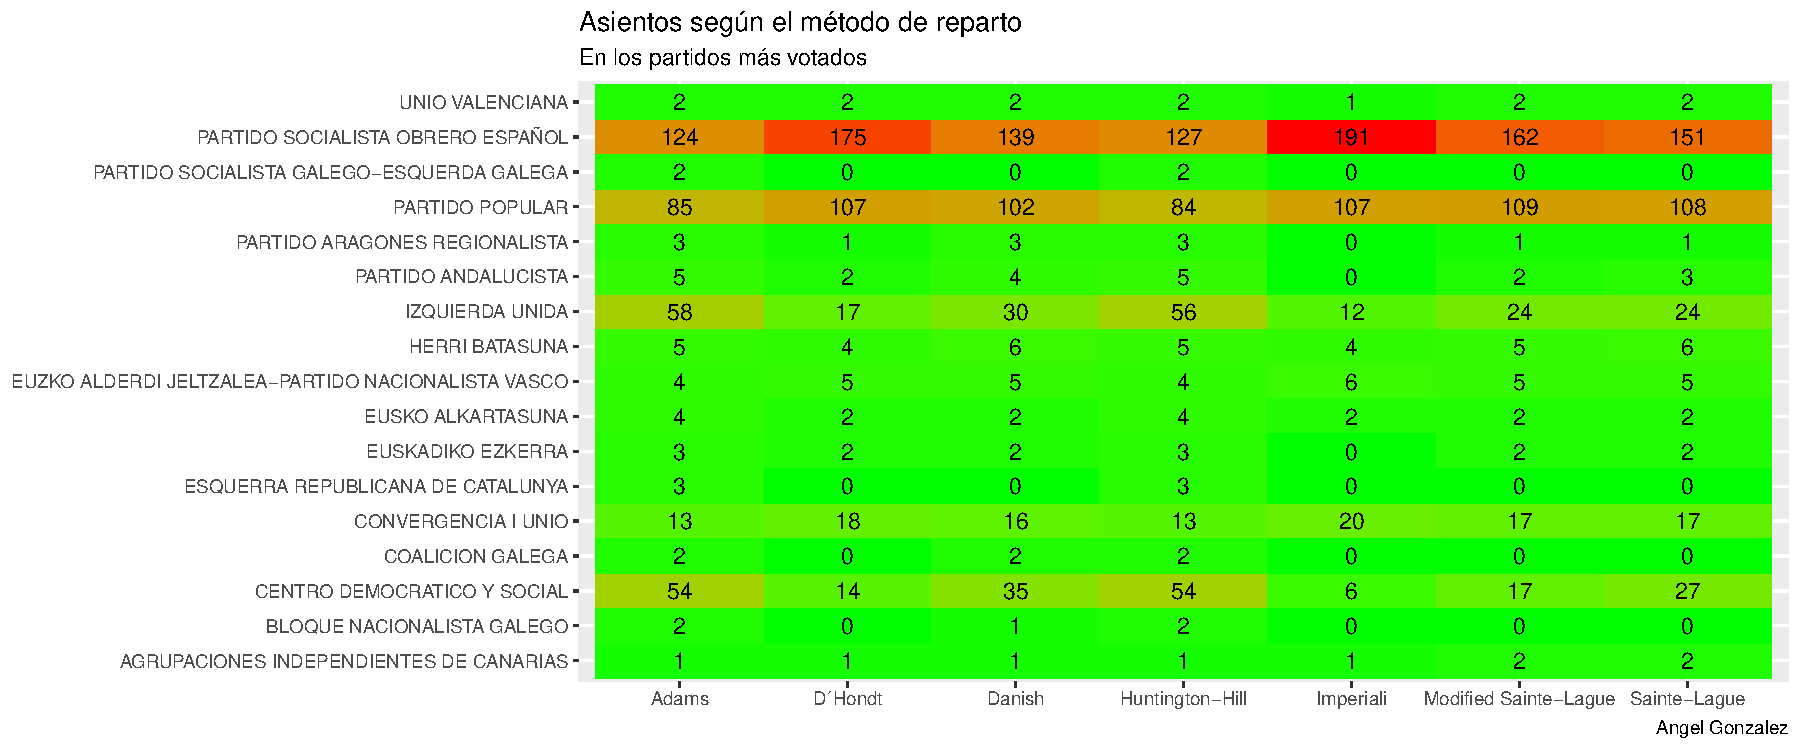
\includegraphics[width=0.95\linewidth]{figurasR/unnamed-chunk-47-2} \end{center}

\begin{center}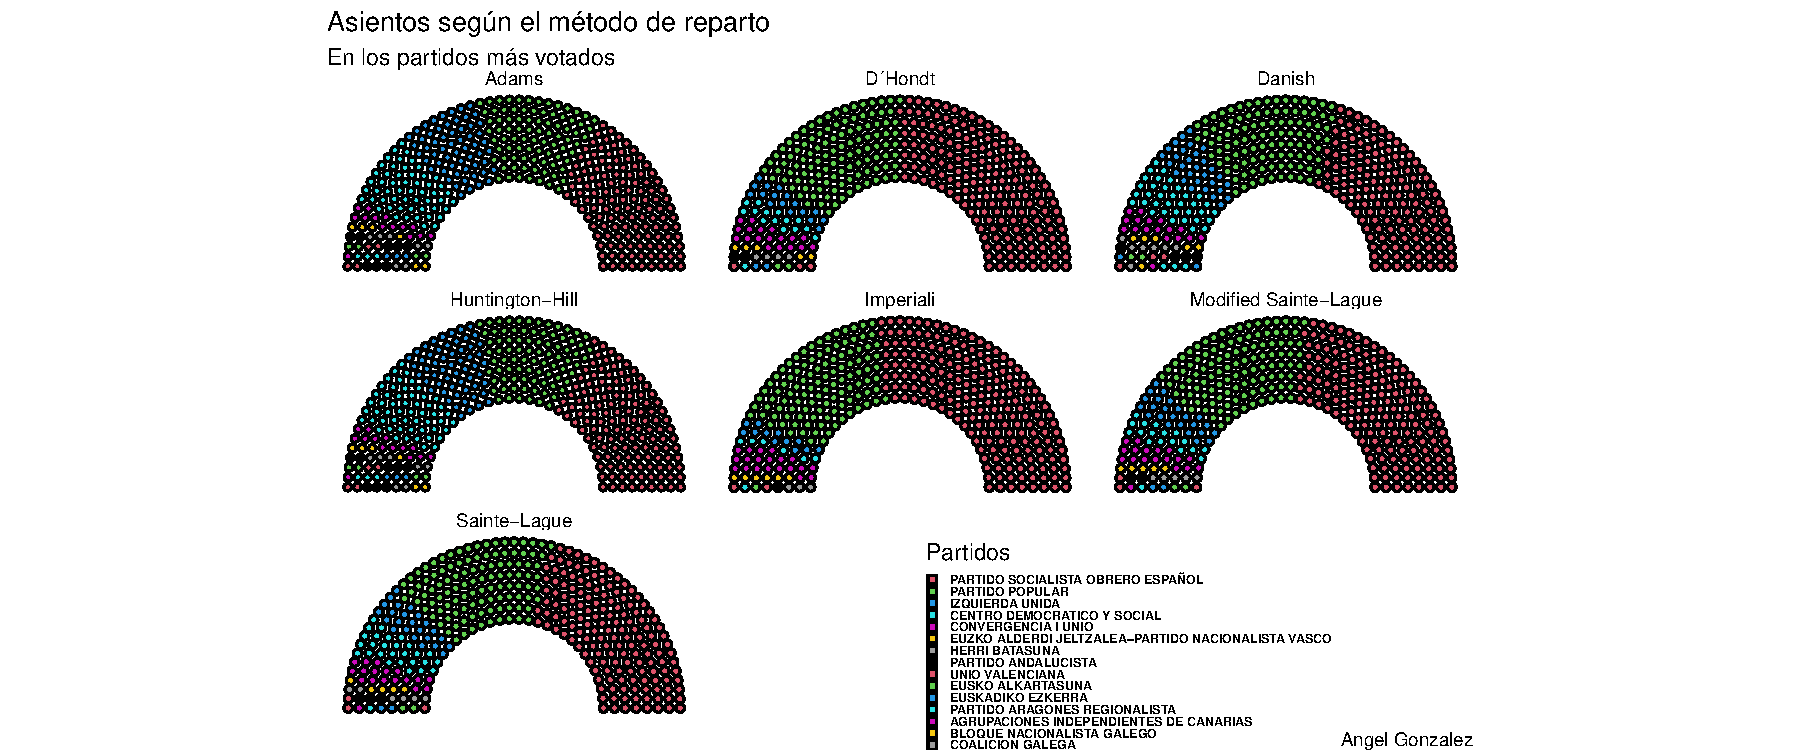
\includegraphics[width=0.95\linewidth]{figurasR/unnamed-chunk-47-3} \end{center}

En estas elecciones de 1989 el partido más votado es, como sucedió el
las anteriores elecciones, el \emph{PSOE}, vemos como aparece por
primera vez el Partido Popular como segunda fuerza tomando el puesto que
antes tenía Coalición Popular, estas elecciones también son muy
bipartidistas aunque se va debilitando ese bipartidismo, ahora podemos
decir que hay dos partidos hegemónicos, PSOE y PP, y tres partidos
medianos, los cuales serían el Centro Democrático y Social, Izquierda
Unida y Convergencia y Unión, de todos estos partidos los más
desfavorecidos por la utilización del método D´Hondt son IU y Centro
Democrático, los cuales de haber utilizado los métodos más
proporcionales podrían hasta duplicar su presencia en el congreso. Por
la otra parte en el caso del PSOE pasaría de alcanzar la mayoría
absoluta justa con 175 escaños a perder la mayoría absoluta en el caso
de optar por los métodos más proporcionales.

\hypertarget{disproporcionalidad-4}{%
\subsubsection{Disproporcionalidad}\label{disproporcionalidad-4}}

\begin{center}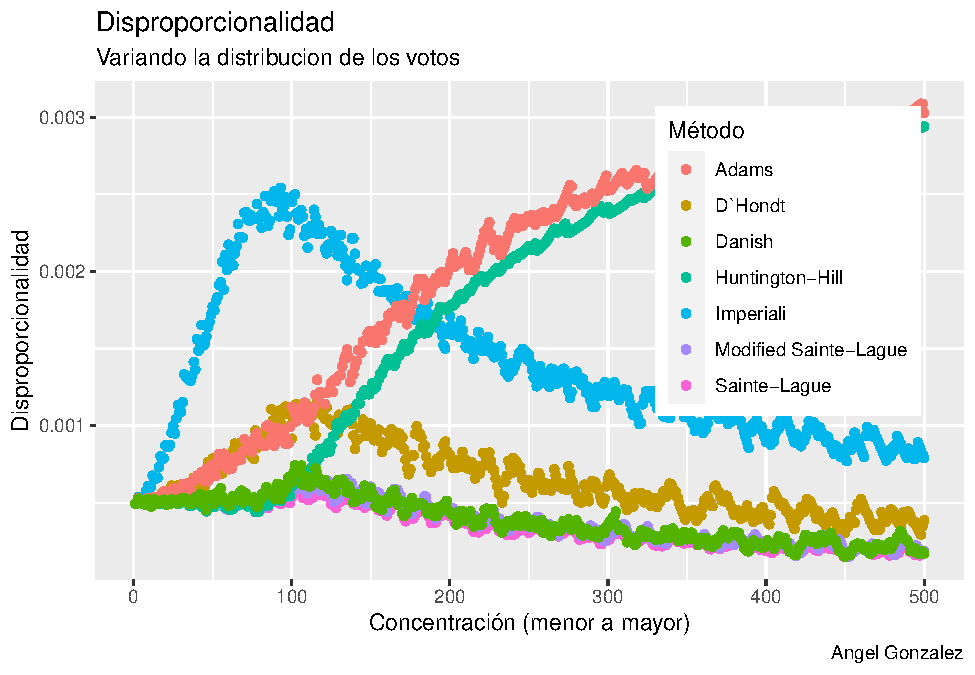
\includegraphics[width=0.95\linewidth]{figurasR/unnamed-chunk-48-1} \end{center}

\begin{center}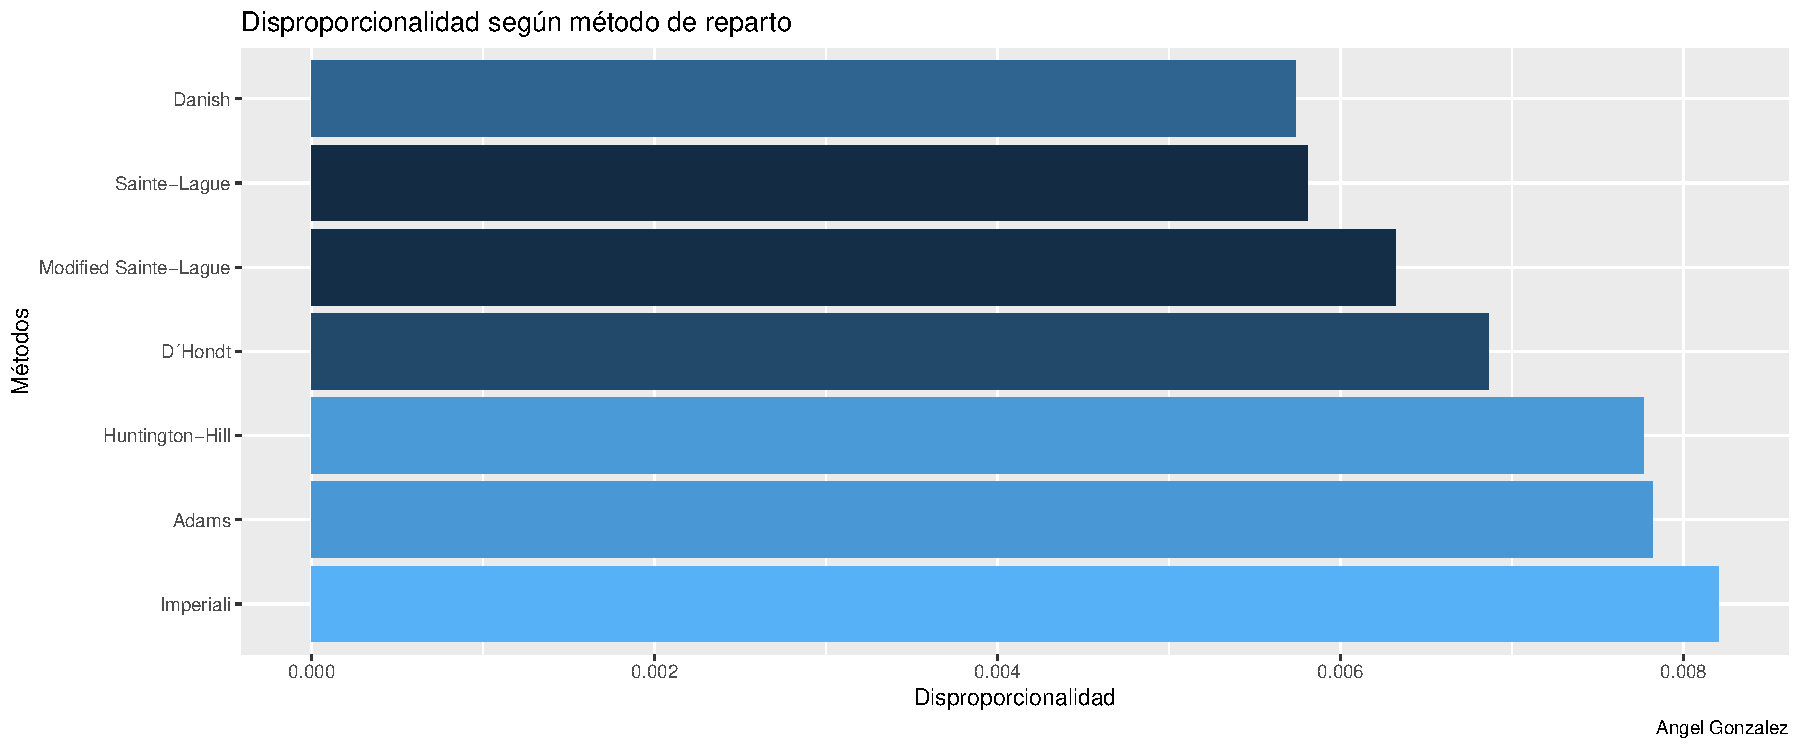
\includegraphics[width=0.95\linewidth]{figurasR/unnamed-chunk-48-2} \end{center}

Este año aunmenta ligeramente la diferencia de disproporción entre
comunidades, sin encontrar novedades en las comunidades más
proporcionales, Madrid, y las más disproporcionadas, las ciudades de
Ceuta y Melilla. Observando los métodos de reparto hay dos grupos
diferenciados, uno en el que se encuentran el método Adams y el método
de huntington-Hill, en los cuales no se encuentran comunidades con picos
de disproporción pero por el lado contrario su disproporción media es
alta, y otro grupo que serían los restantes métodos los cuales todos
presentan unos mismos picos máximos como míninos.

Estas elecciones de 1989 la disproporcionalidad media se agrupa en tres
grupos, alta, media y baja disproporción, el más disproporcionado vuelve
a ser el método Imperiali, el método D´Hondt sigue en el grupo medio y
el método más proporcionado vuelve a ser el Danish aunque le sigue muy
cerca el método Sainte-Lague.

\hypertarget{auxf1o-1993}{%
\section{Año 1993}\label{auxf1o-1993}}

\hypertarget{comparativa-entre-muxe9todos-5}{%
\subsection{Comparativa entre
métodos}\label{comparativa-entre-muxe9todos-5}}

\hypertarget{votos-obtenidos-5}{%
\subsubsection{Votos obtenidos}\label{votos-obtenidos-5}}

\begin{center}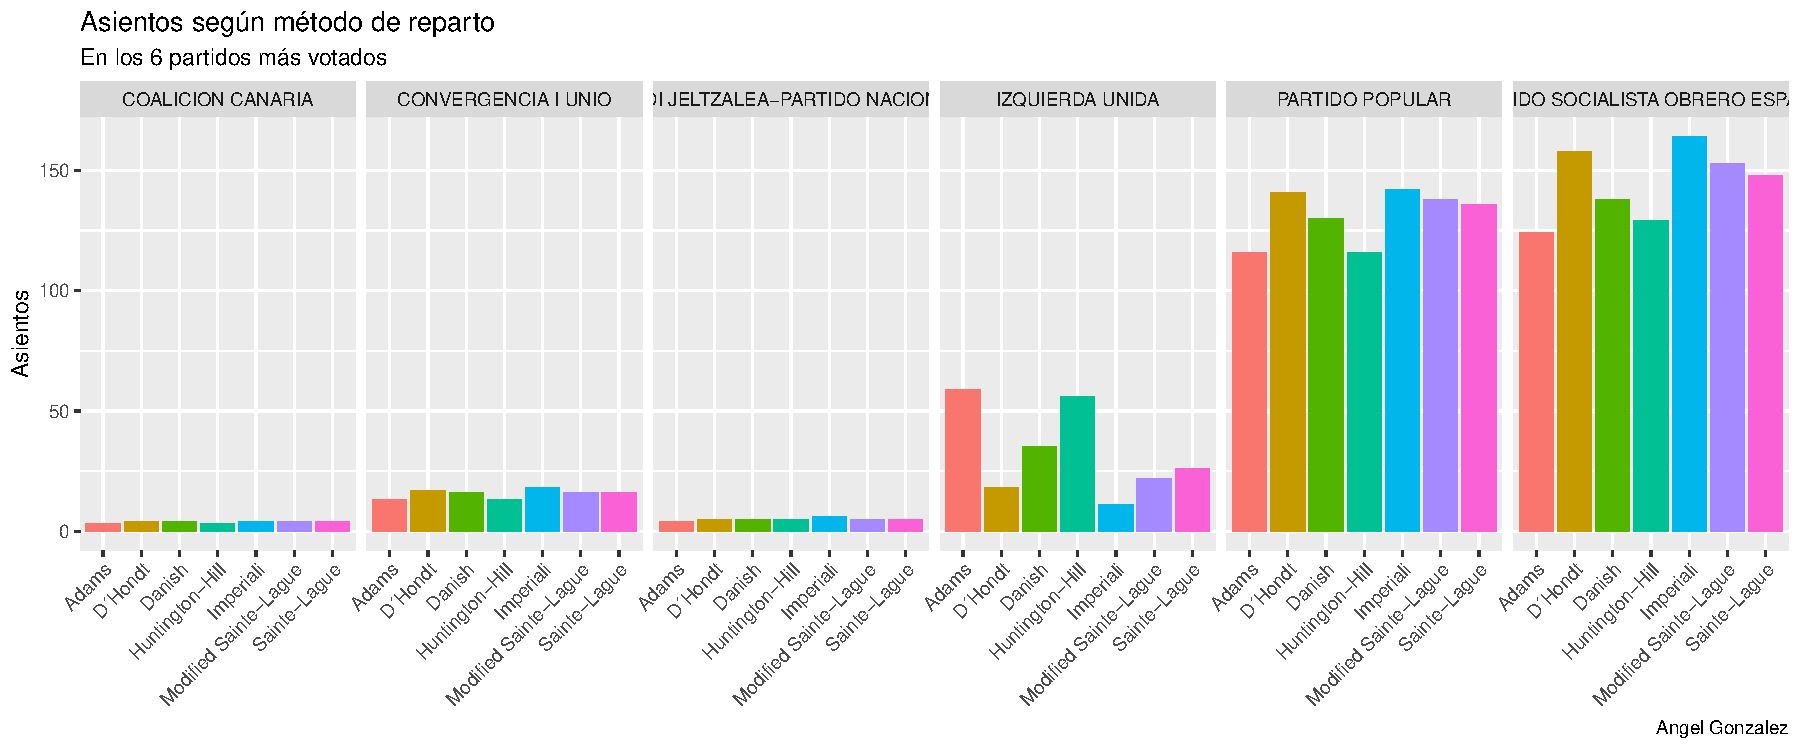
\includegraphics[width=0.95\linewidth]{figurasR/unnamed-chunk-56-1} \end{center}

\begin{center}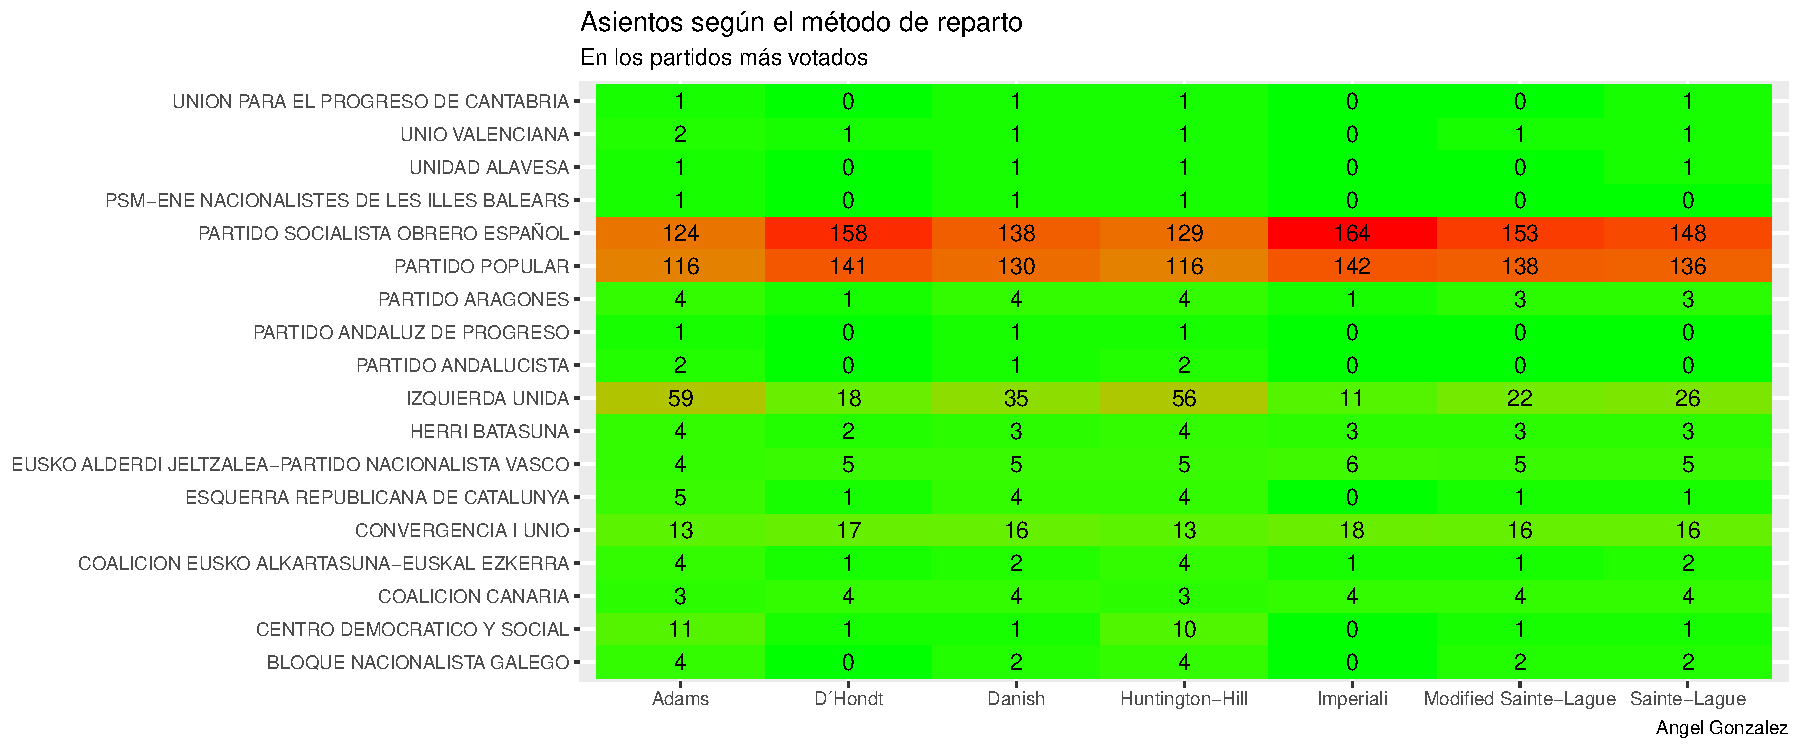
\includegraphics[width=0.95\linewidth]{figurasR/unnamed-chunk-56-2} \end{center}

\begin{center}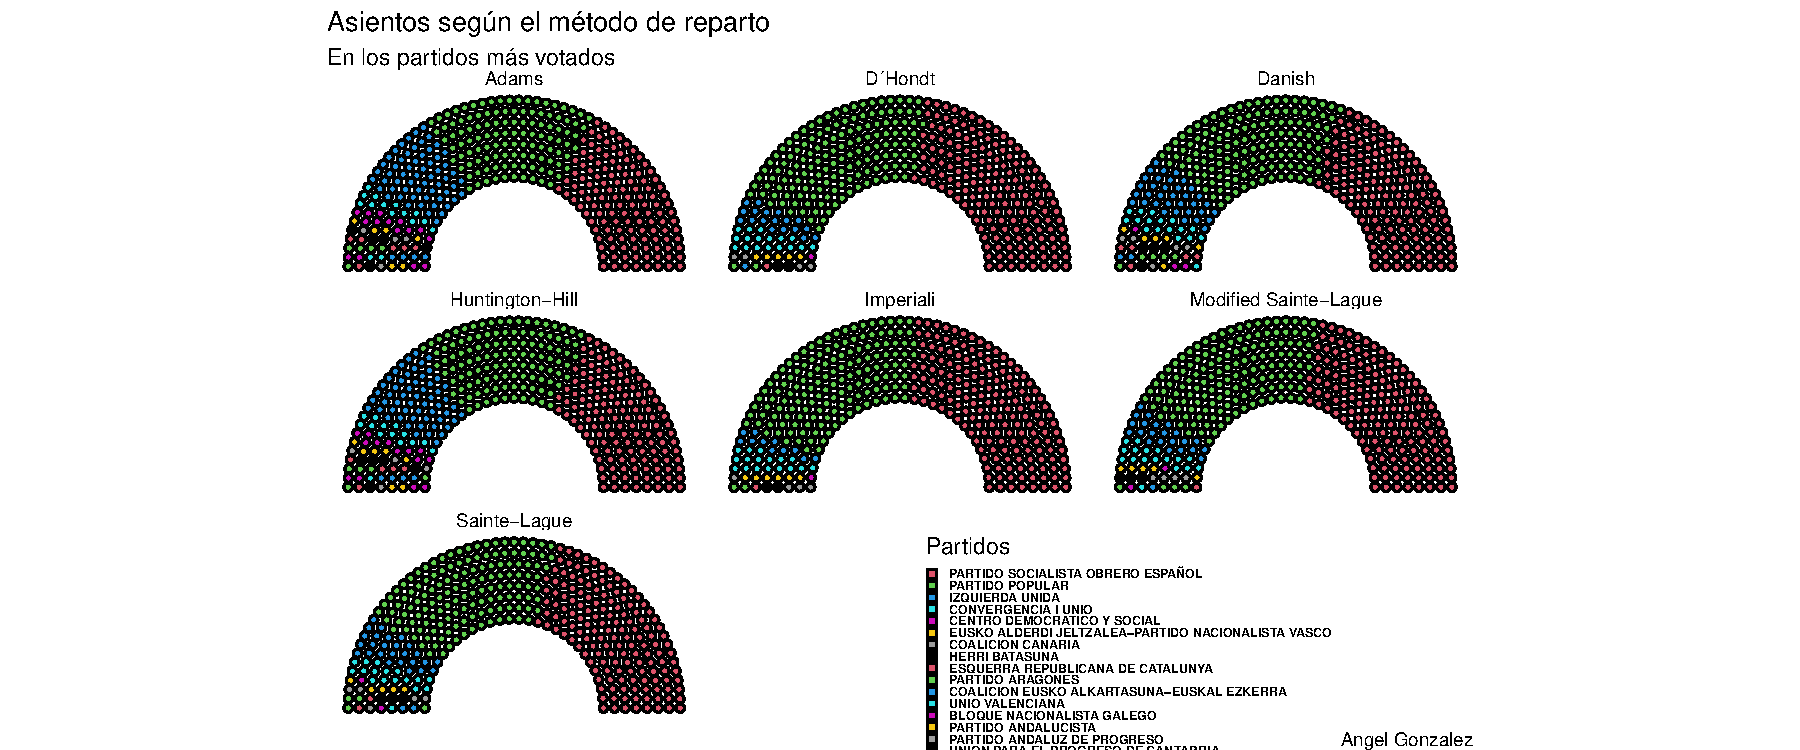
\includegraphics[width=0.95\linewidth]{figurasR/unnamed-chunk-56-3} \end{center}

En las elecciones de 1993 podemos observar como la fuerza del primer
partido va decreciendo lentamente. Los dos partidos más votados son el
\emph{PSOE} y el \emph{PP} respectivamente, la diferencia estas
elecciones es que el PSOE ha perdido la mayoría absoluta según el método
D´Hondt y en cambio el PP ha aumentado su presencia significativamente y
está ya relativamente cerca de alcanzar al PSOE. De haber utilizado los
métodos más proporcionales resultaría en una menor diferencia de escaños
entre estos dos grandes partidos, el partido más castigado en estas
elecciones sigue siendo IU, el cual podría haber obtenido de 1.5 a 2
veces más asientos de haber cambiado de método de reparto. Son unas
elecciones en donde hay dos partidos hegemónicos y dos partidos medianos
que son IU y CIU, como hemos visto IU es un partido muy castigado por el
método de reparto actual, en cambio CiU no se vería agraviado o
beneficiado al cambiar el método de reparto.

\hypertarget{disproporcionalidad-5}{%
\subsubsection{Disproporcionalidad}\label{disproporcionalidad-5}}

\begin{center}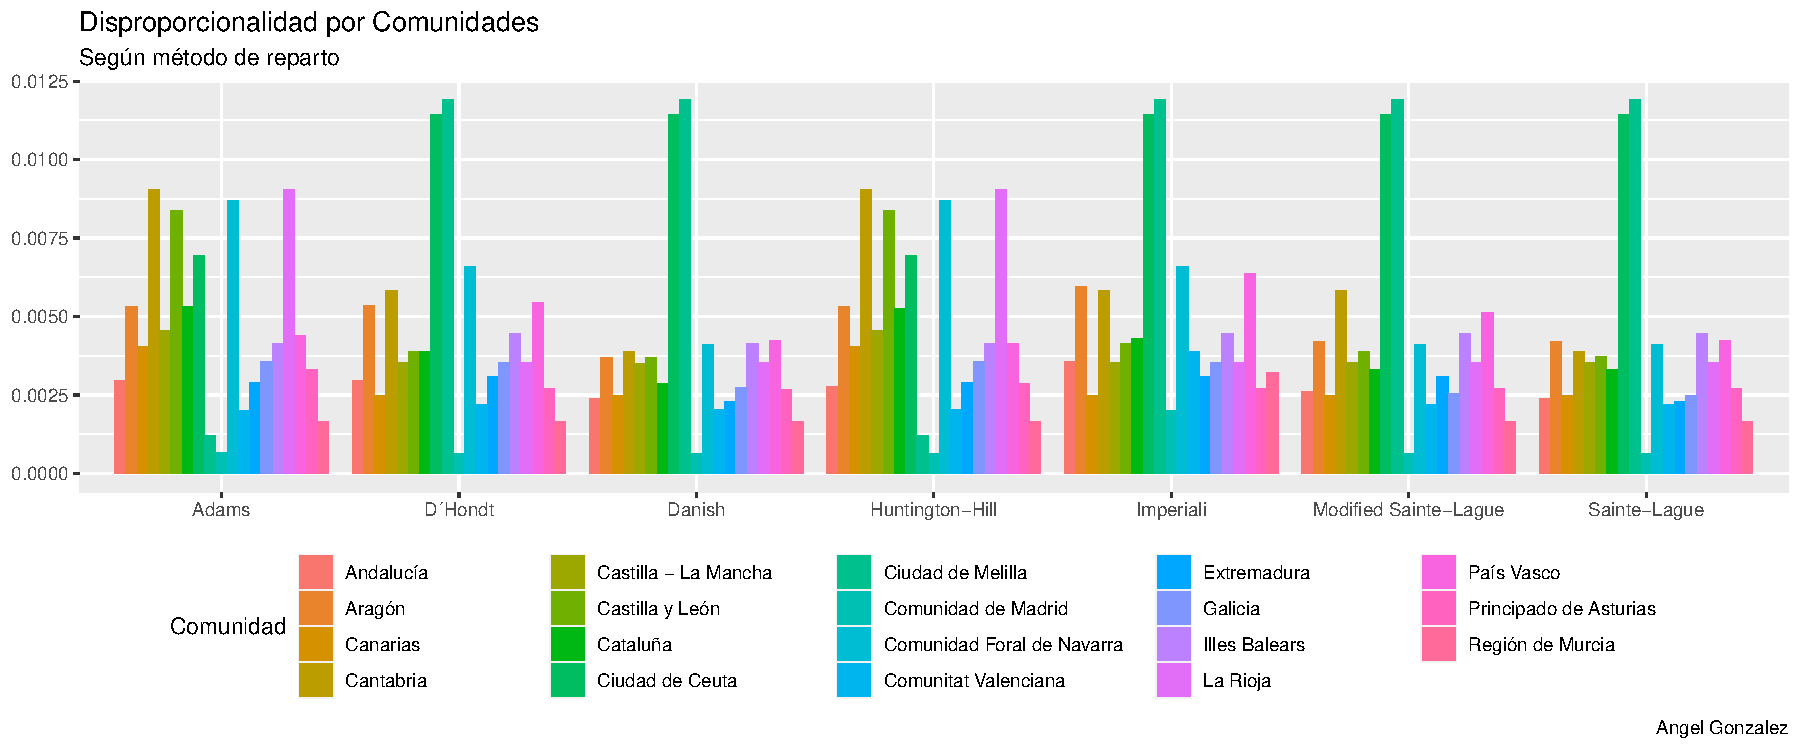
\includegraphics[width=0.95\linewidth]{figurasR/unnamed-chunk-57-1} \end{center}

\begin{center}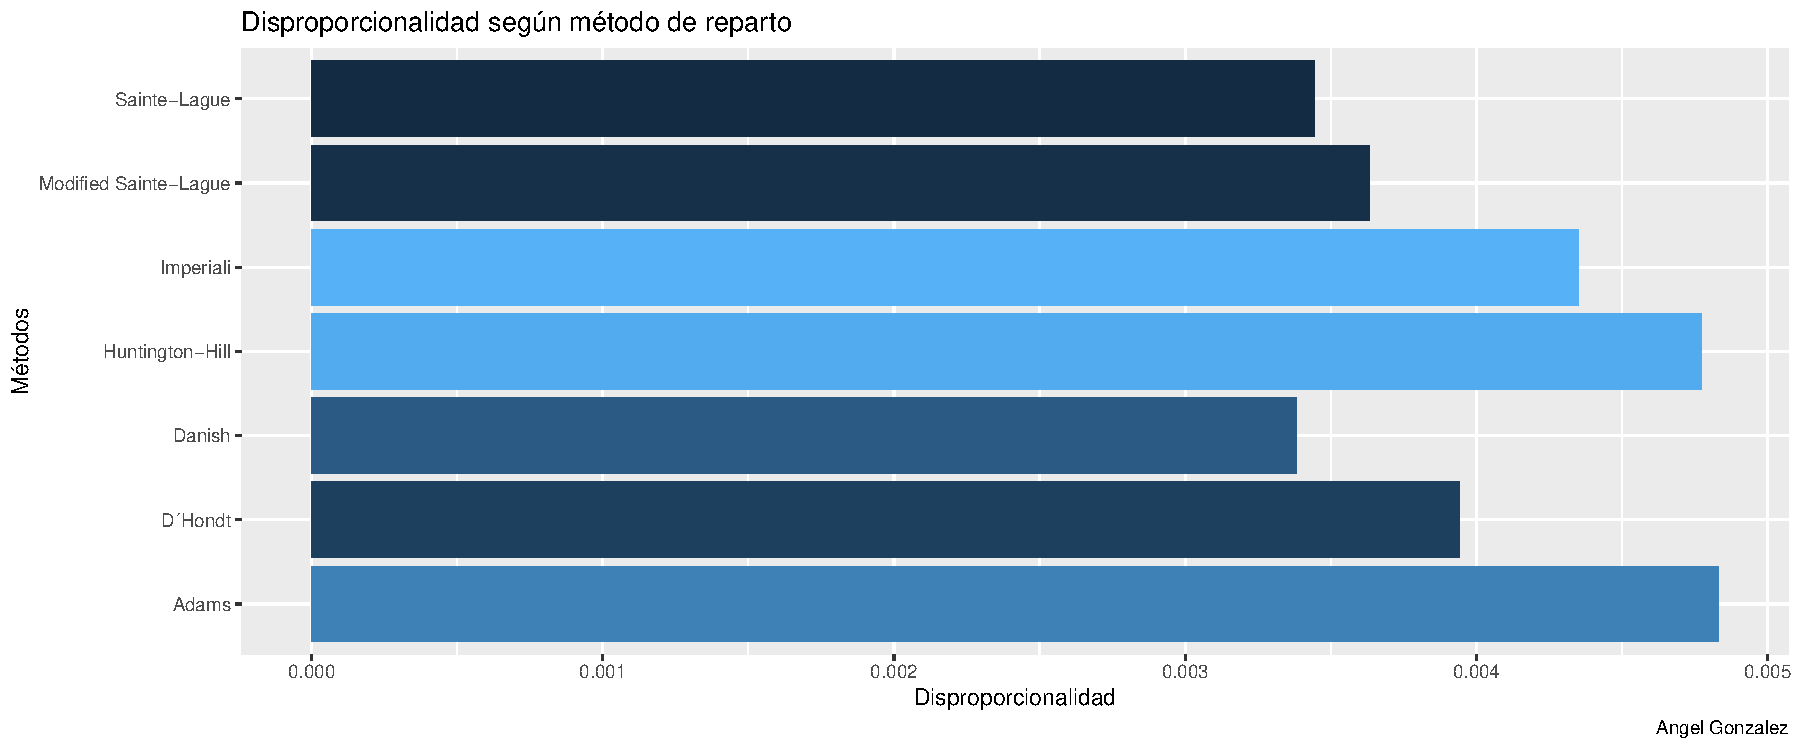
\includegraphics[width=0.95\linewidth]{figurasR/unnamed-chunk-57-2} \end{center}

En estas elecciones se observan más picos de disproporción en
comparación con las elecciones anteriores, especialmente aumenta su
disproporción el Pais Vasco y Aragón, no hay novedades en los máximos ni
en los mínimos.

Este año en el caso de la disproporcionalidad media según el método de
reparto vemos que hay diferencias en los métodos más disproporcionales,
usualmente el método más disproporcionado ha sido el Imperiali, en estas
elecciones esto cambia, de hecho mejora en dos puestos. Los más
disproporcionados este año entonces son los métodos Adams y de
Huntington-Hill, en el caso de los más proporcionados no hay novedades,
sigue siendo el método Danish seguido muy de cerca por el Sainte-Lague.

\hypertarget{auxf1o-1996}{%
\section{Año 1996}\label{auxf1o-1996}}

\hypertarget{comparativa-entre-muxe9todos-6}{%
\subsection{Comparativa entre
métodos}\label{comparativa-entre-muxe9todos-6}}

\hypertarget{votos-obtenidos-6}{%
\subsubsection{Votos obtenidos}\label{votos-obtenidos-6}}

\begin{center}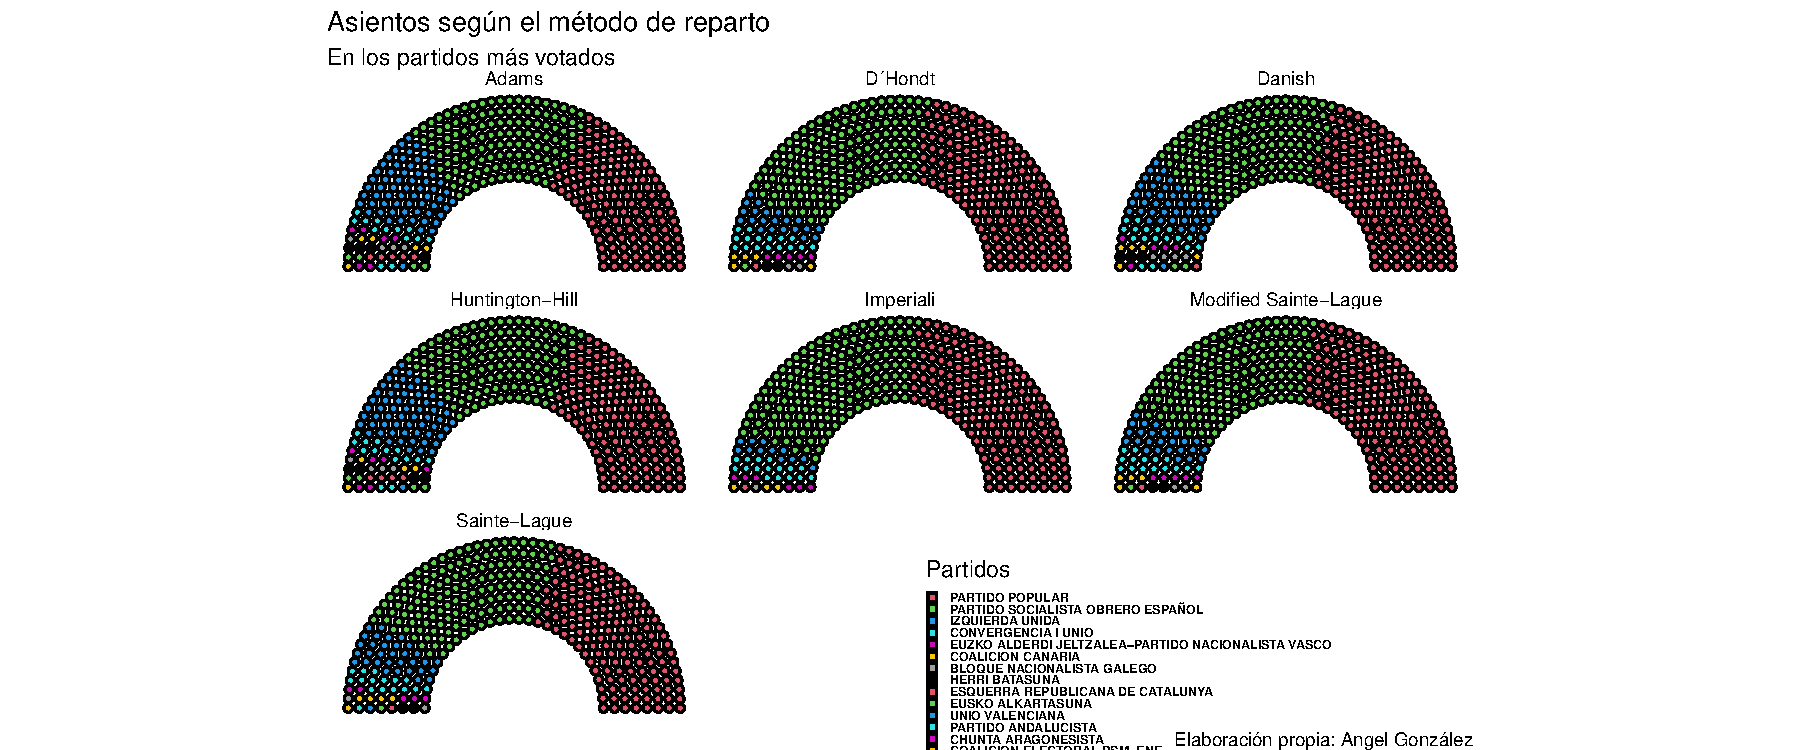
\includegraphics[width=0.95\linewidth]{figurasR/unnamed-chunk-65-1} \end{center}

\begin{center}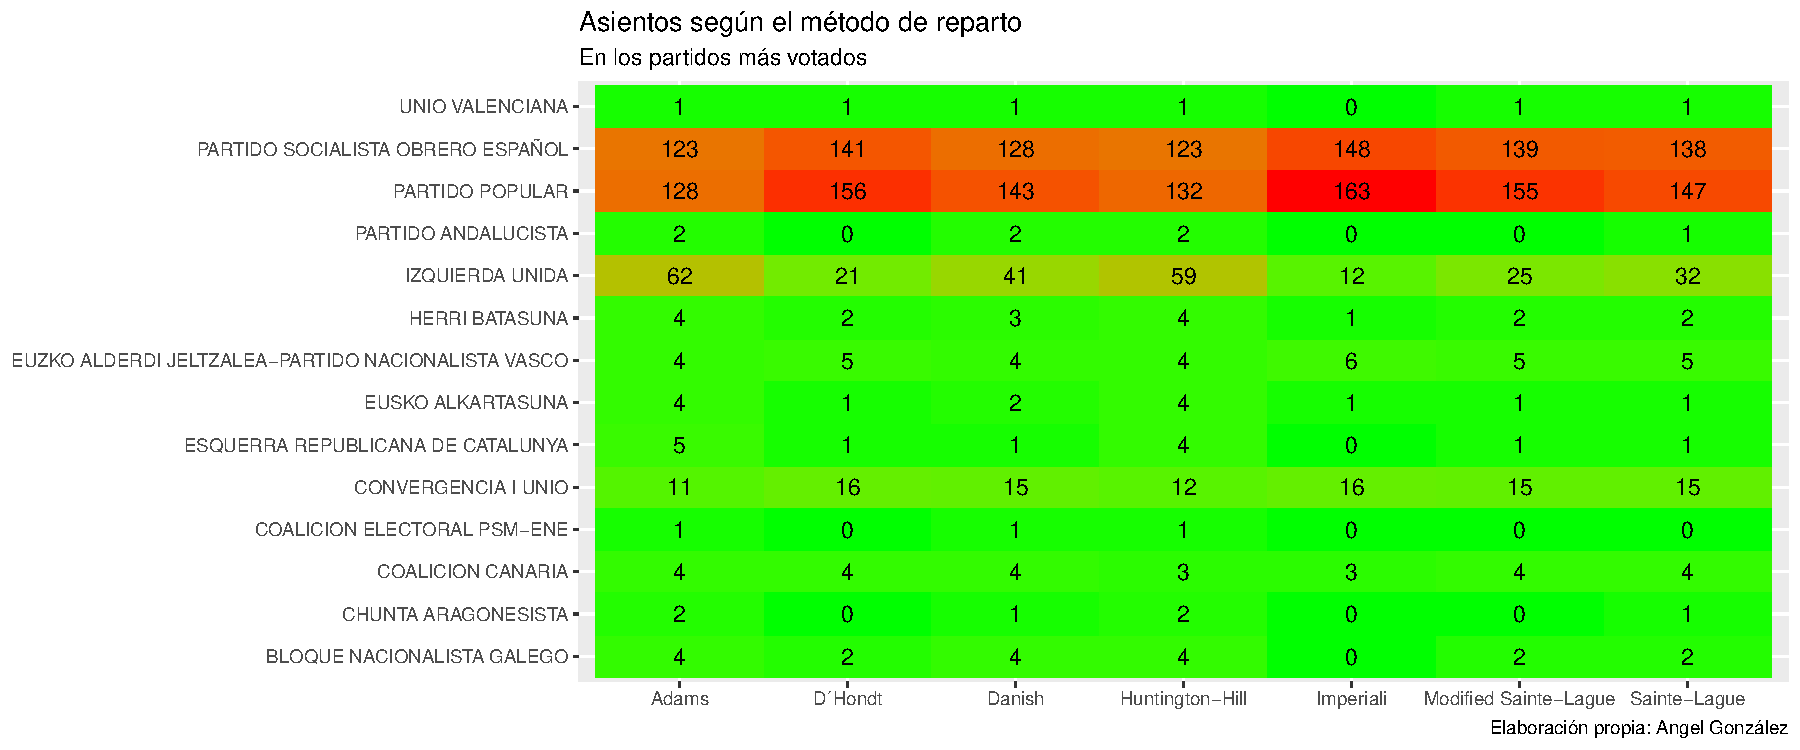
\includegraphics[width=0.95\linewidth]{figurasR/unnamed-chunk-65-2} \end{center}

\begin{center}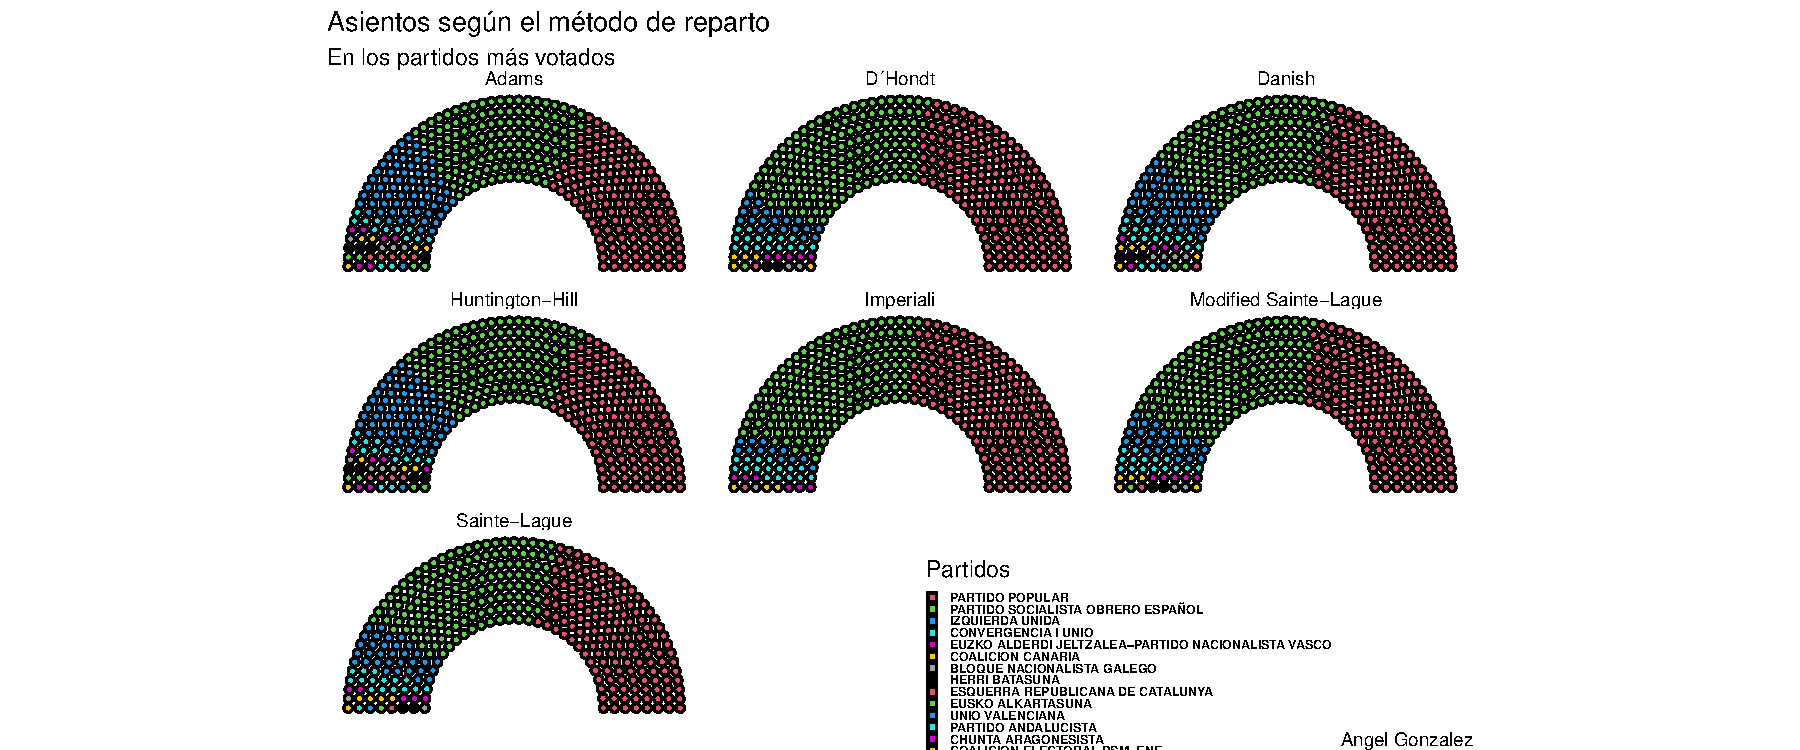
\includegraphics[width=0.95\linewidth]{figurasR/unnamed-chunk-65-3} \end{center}

En estas elecciones de 1996 son las primeras elecciones en donde el
\emph{PP} son la fuerza más votada, el \emph{PSOE} que ya llevaba una
tendencia descendiente al final ha perdido el primer puesto. Sigue
habiendo un bipartidismo significativo con dos partidos medianos,
todavía el PP a pesar de ganar las elecciones no alcanza la mayoría
absoluta en ninguno de los métodos analizados

\hypertarget{disproporcionalidad-6}{%
\subsubsection{Disproporcionalidad}\label{disproporcionalidad-6}}

\begin{center}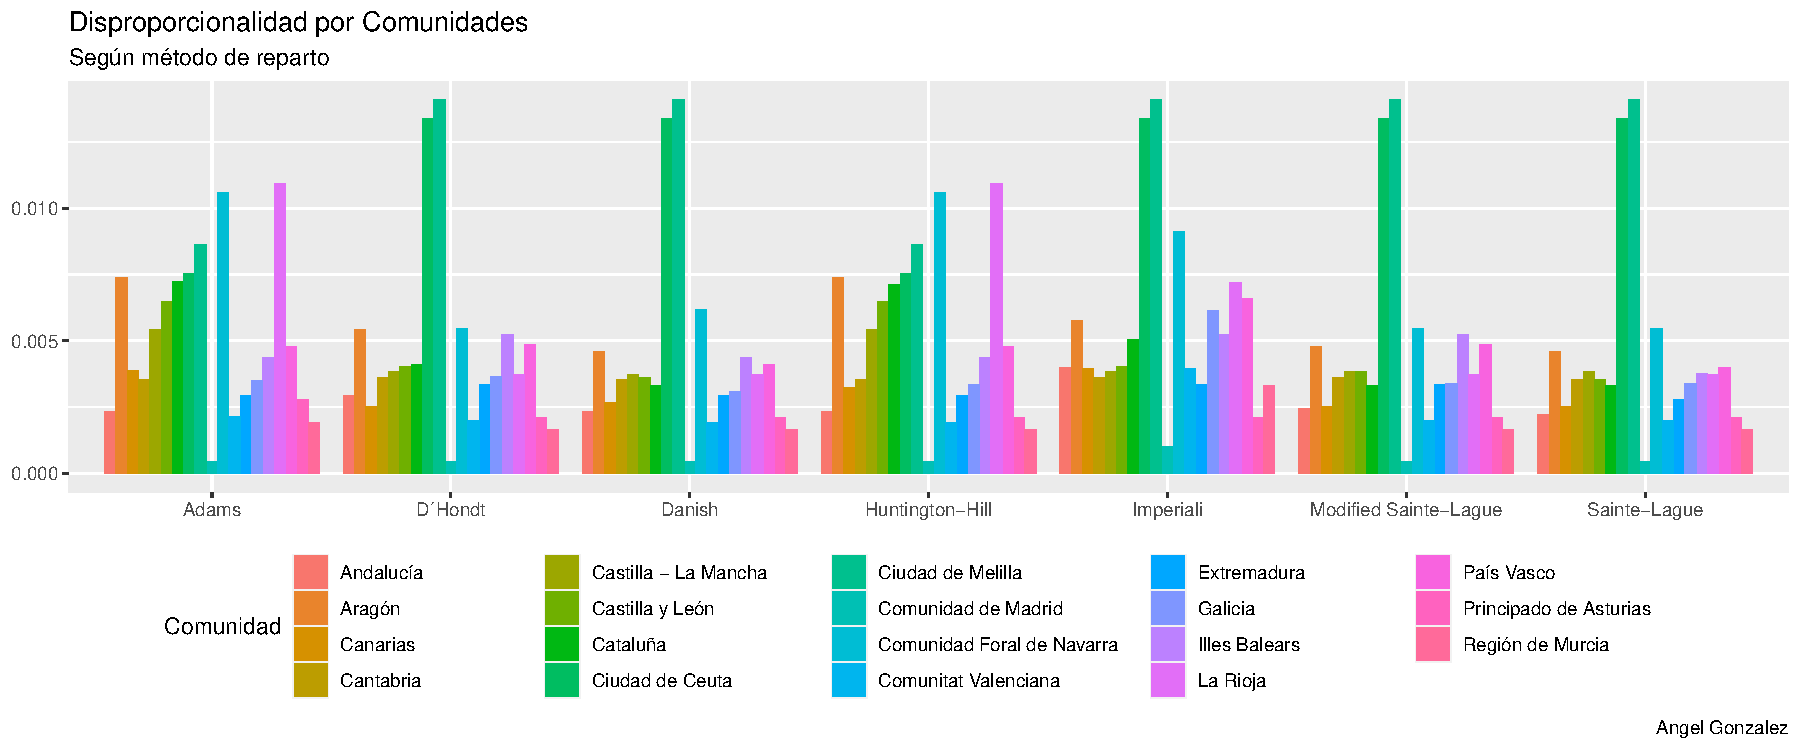
\includegraphics[width=0.95\linewidth]{figurasR/unnamed-chunk-66-1} \end{center}

\begin{center}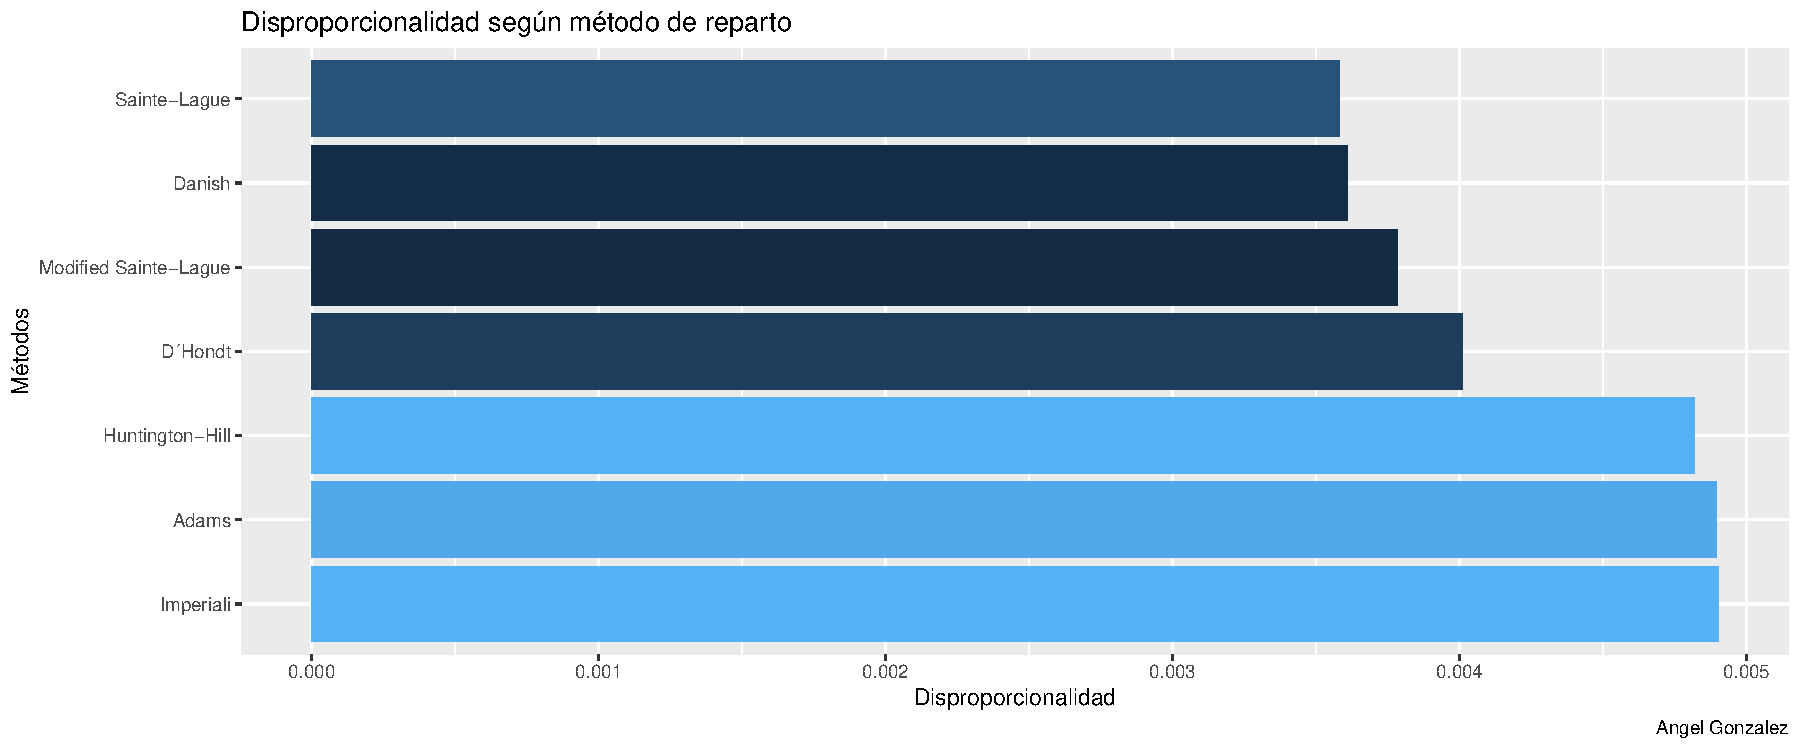
\includegraphics[width=0.95\linewidth]{figurasR/unnamed-chunk-66-2} \end{center}

\hypertarget{auxf1o-2000}{%
\section{Año 2000}\label{auxf1o-2000}}

\hypertarget{comparativa-entre-muxe9todos-7}{%
\subsection{Comparativa entre
métodos}\label{comparativa-entre-muxe9todos-7}}

\hypertarget{votos-obtenidos-7}{%
\subsubsection{Votos obtenidos}\label{votos-obtenidos-7}}

\begin{center}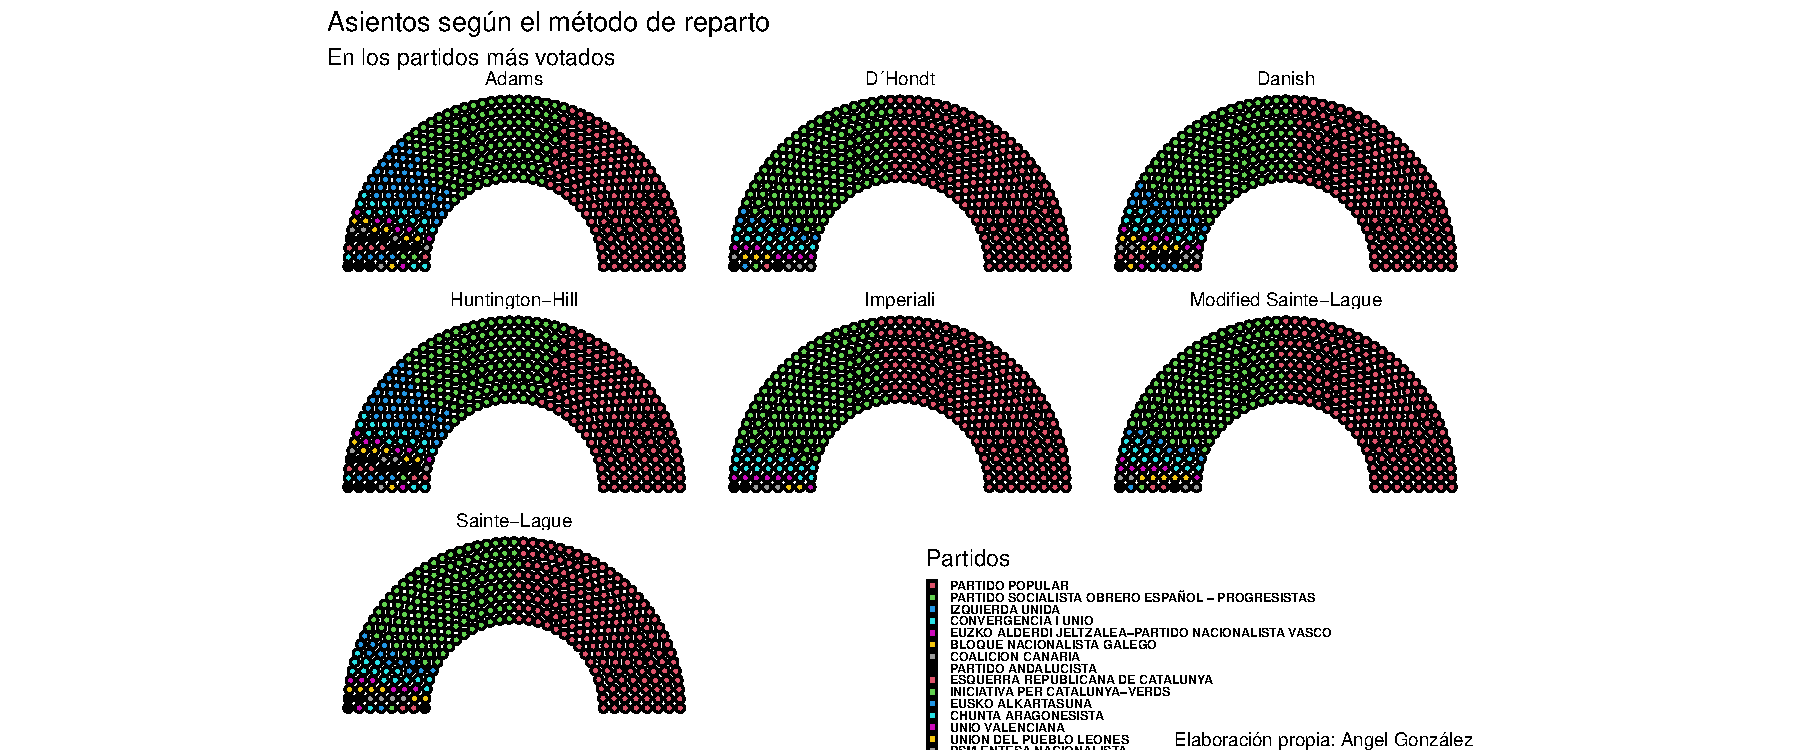
\includegraphics[width=0.95\linewidth]{figurasR/unnamed-chunk-74-1} \end{center}

\begin{center}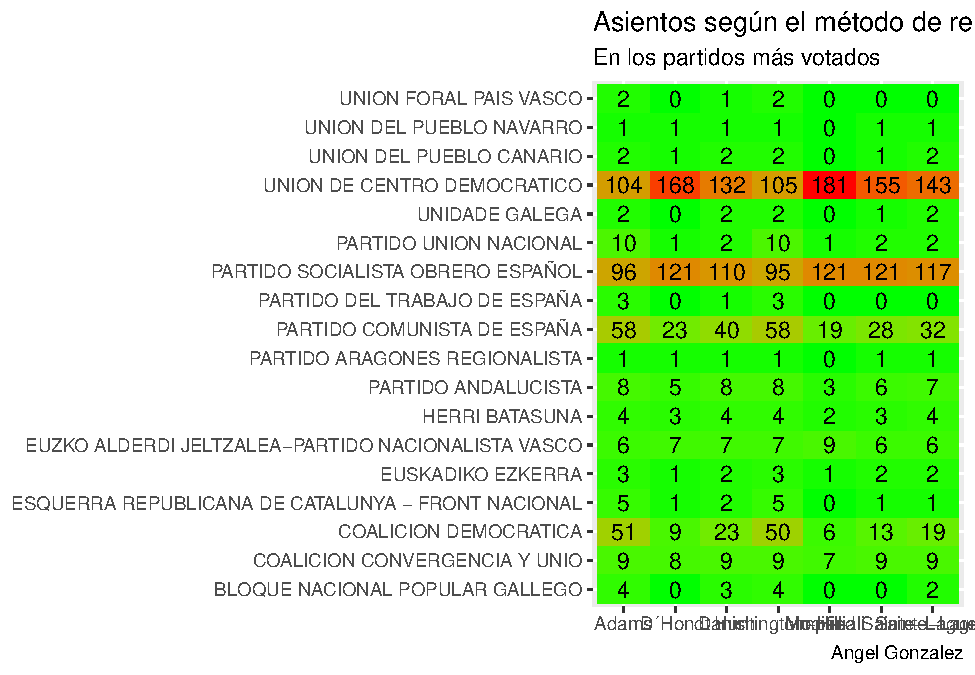
\includegraphics[width=0.95\linewidth]{figurasR/unnamed-chunk-74-2} \end{center}

\begin{center}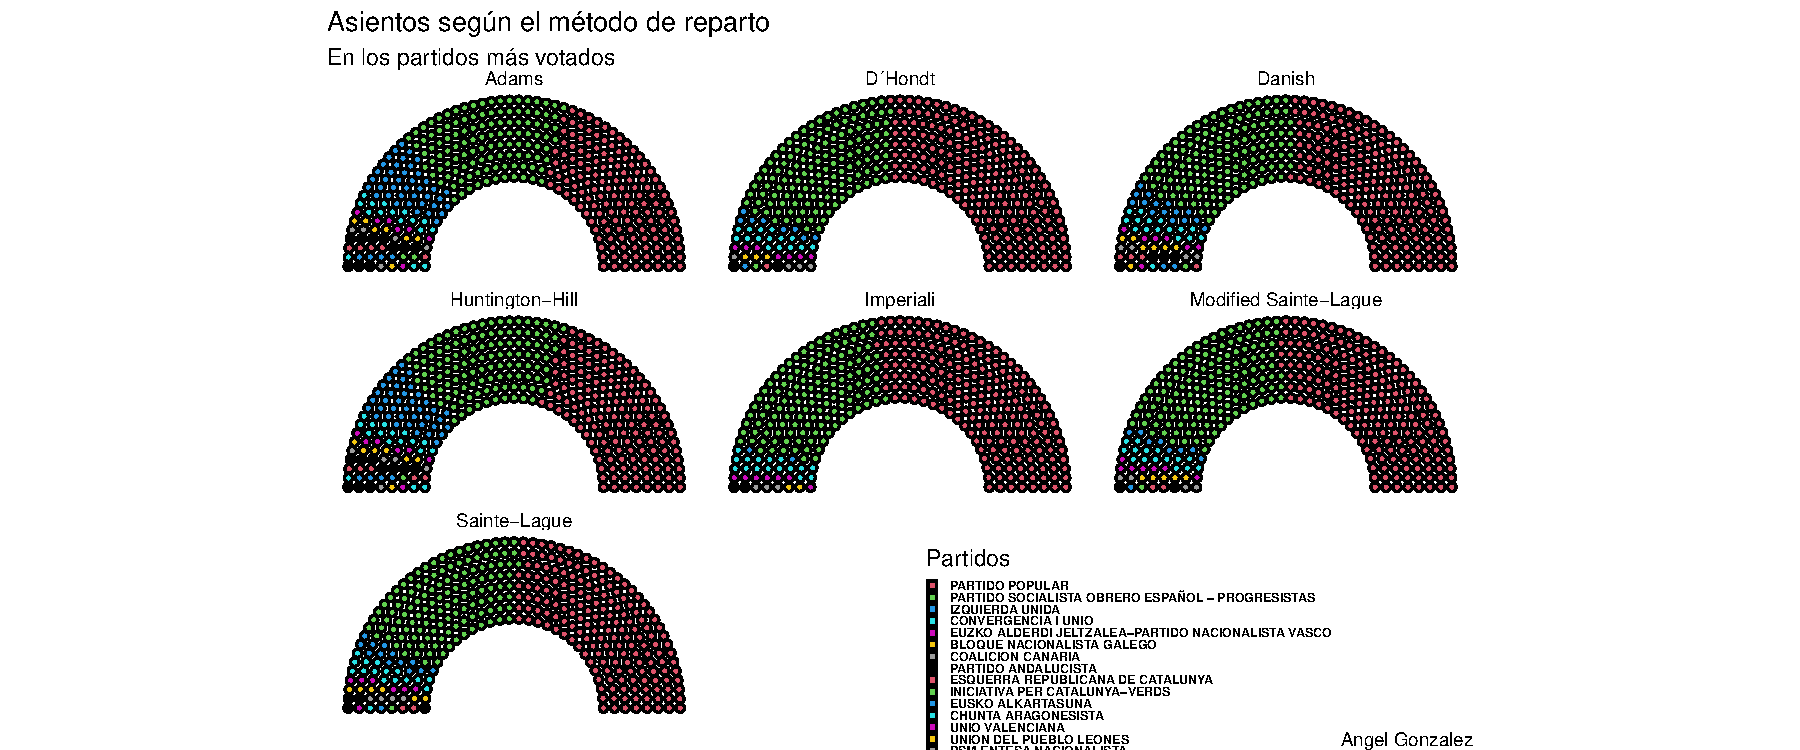
\includegraphics[width=0.95\linewidth]{figurasR/unnamed-chunk-74-3} \end{center}

En las elecciones del año 2000 el partido más votado vuelve a ser el
\emph{Partido Popular} seguido del \emph{PSOE}, en estas elecciones
según el método D´Hondt utilizado en España el PP conseguiría una
mayoría absoluta holgada, es una elección con un claro bipartidismo
donde se podría decir que no existen partidos medianos. Si optasemos por
otro método de reparto más proporcional como puede ser el método Danish
o el Sainte-Lague el PP no alcanzaría la mayoría absoluta, se quedaría a
muy pocos escaños de alcanzarla, en cambio veríamos a muchos partidos
pequeños con menos de tres votos casi duplicar su presencia en escaños.
El partido más castigado por utilizar el método D´Hondt en estas
elecciones sigue siendo Izquierda Unida.

\hypertarget{disproporcionalidad-7}{%
\subsubsection{Disproporcionalidad}\label{disproporcionalidad-7}}

\begin{center}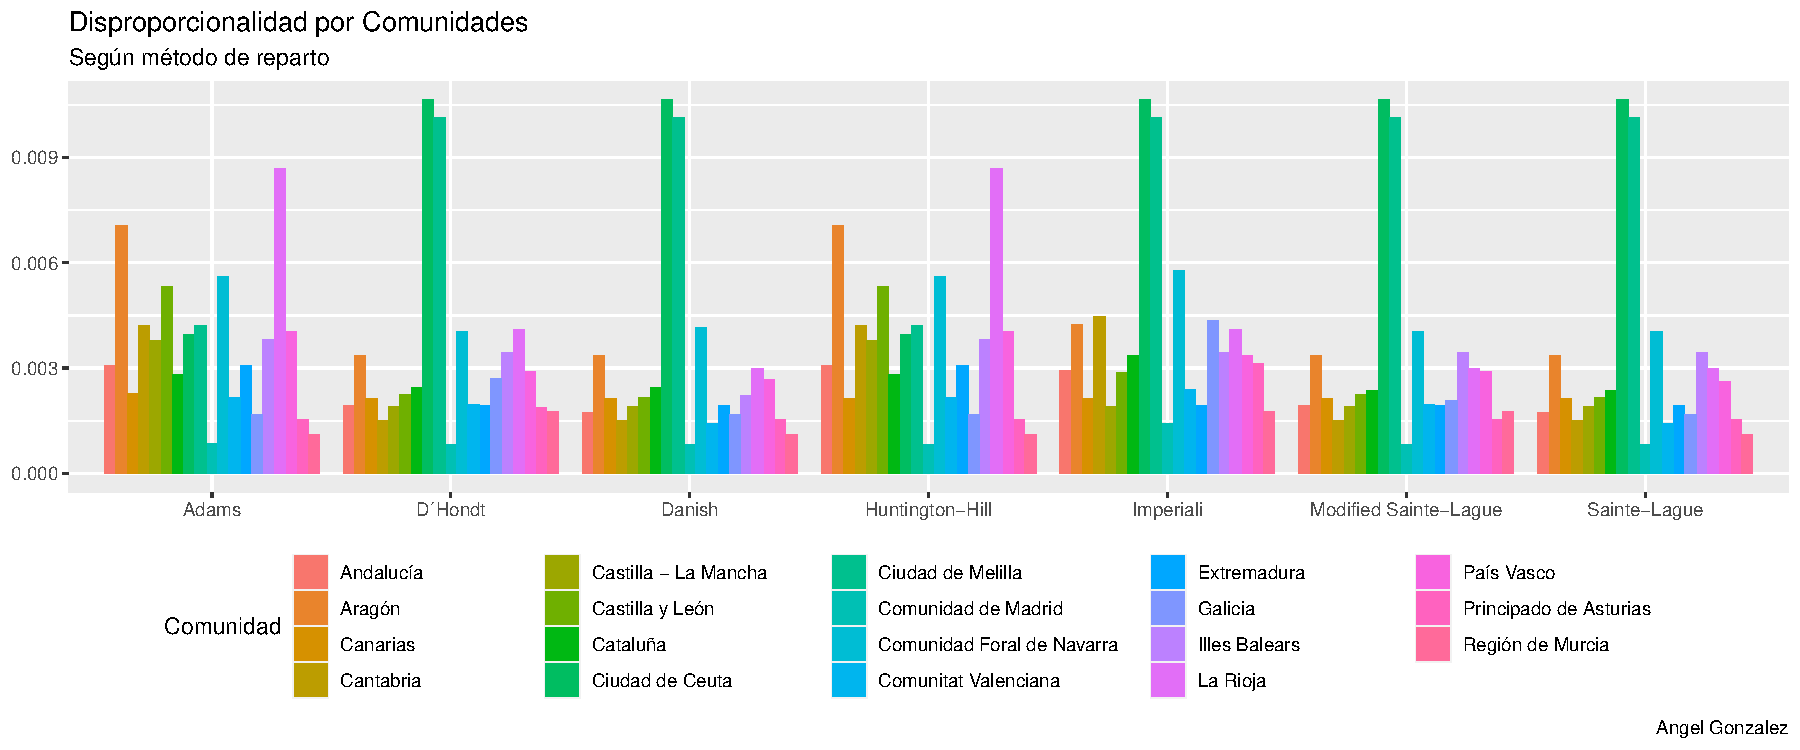
\includegraphics[width=0.95\linewidth]{figurasR/unnamed-chunk-75-1} \end{center}

\begin{center}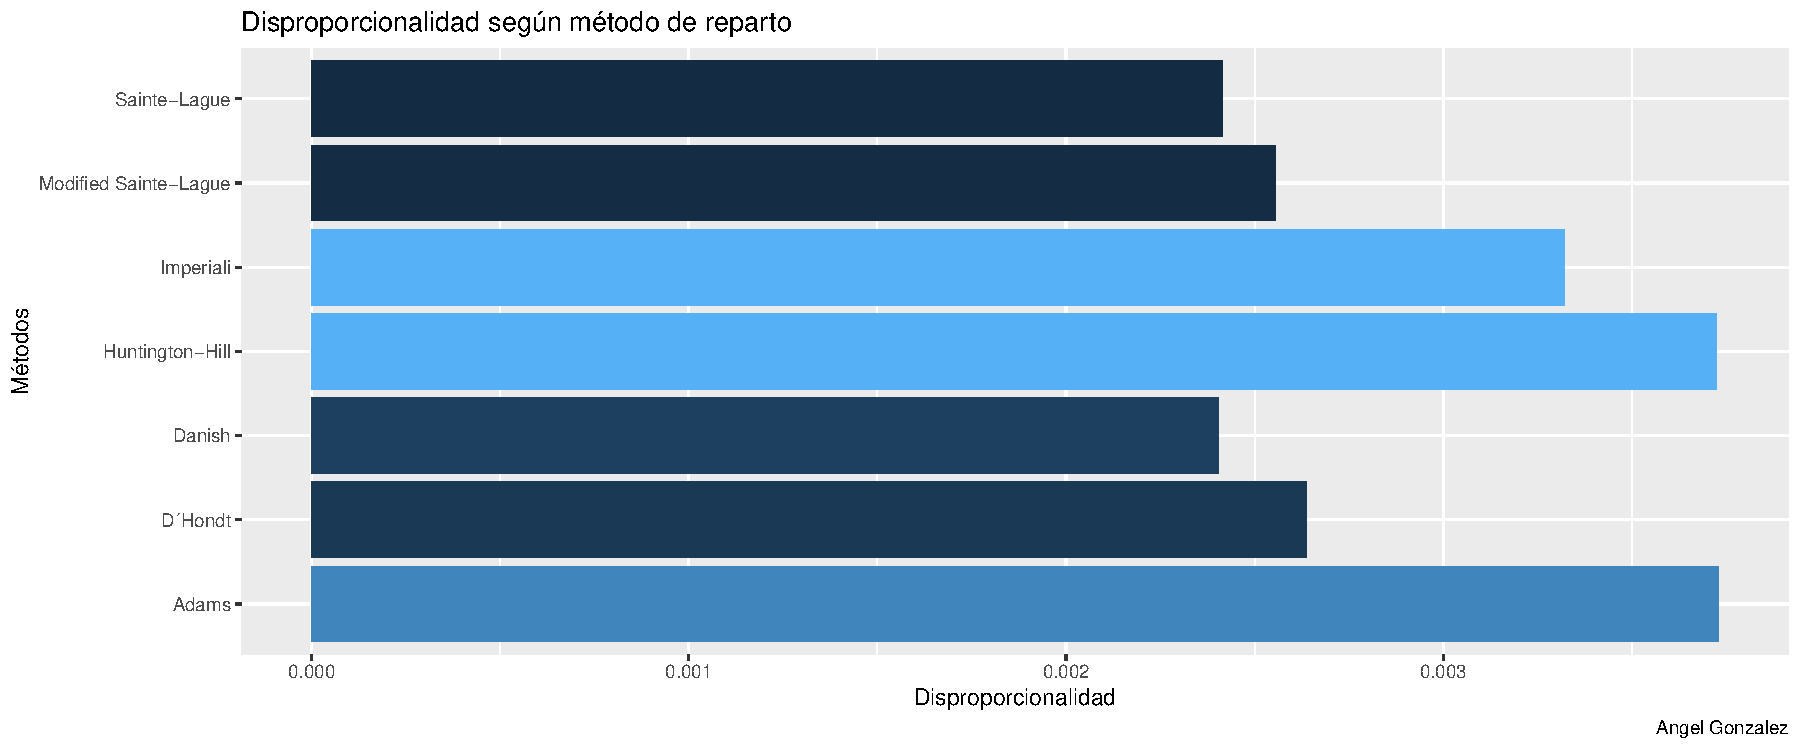
\includegraphics[width=0.95\linewidth]{figurasR/unnamed-chunk-75-2} \end{center}

Observando la disproporción por comunidades no encontramos diferencias
significativas respecto a las anteriores elecciones, es decir, tanto el
método Adams como el Huntington-Hill tienen un comportamiento diferente
respecto a los demás, siguen siendo los más despropocionados las
ciudades de Ceuta y Melilla, y la más proporcionada la Comunidad de
Madrid, este año es especialmente alta la disproporción de las Islas
Baleares respecto a anteriores elecciones.

Si miramos la gráfica de la disproporcionalidad según el método de
reparto se pueden agrupar los métodos en dos grupos, uno con gran
disproporcionalidad en el que estarían incluidos los métodos Adams,
Imperiali y Huntington-Hill, y el otro grupo restante con una
disproporción media baja. Seguimos observando que el método D´Hont no es
el mejor aunque en estas elecciones se puede considerar un método
aceptable siendo el mejor método alternativo el Danish.

\hypertarget{auxf1o-2004}{%
\section{Año 2004}\label{auxf1o-2004}}

\hypertarget{comparativa-entre-muxe9todos-8}{%
\subsection{Comparativa entre
métodos}\label{comparativa-entre-muxe9todos-8}}

\hypertarget{votos-obtenidos-8}{%
\subsubsection{Votos obtenidos}\label{votos-obtenidos-8}}

\begin{center}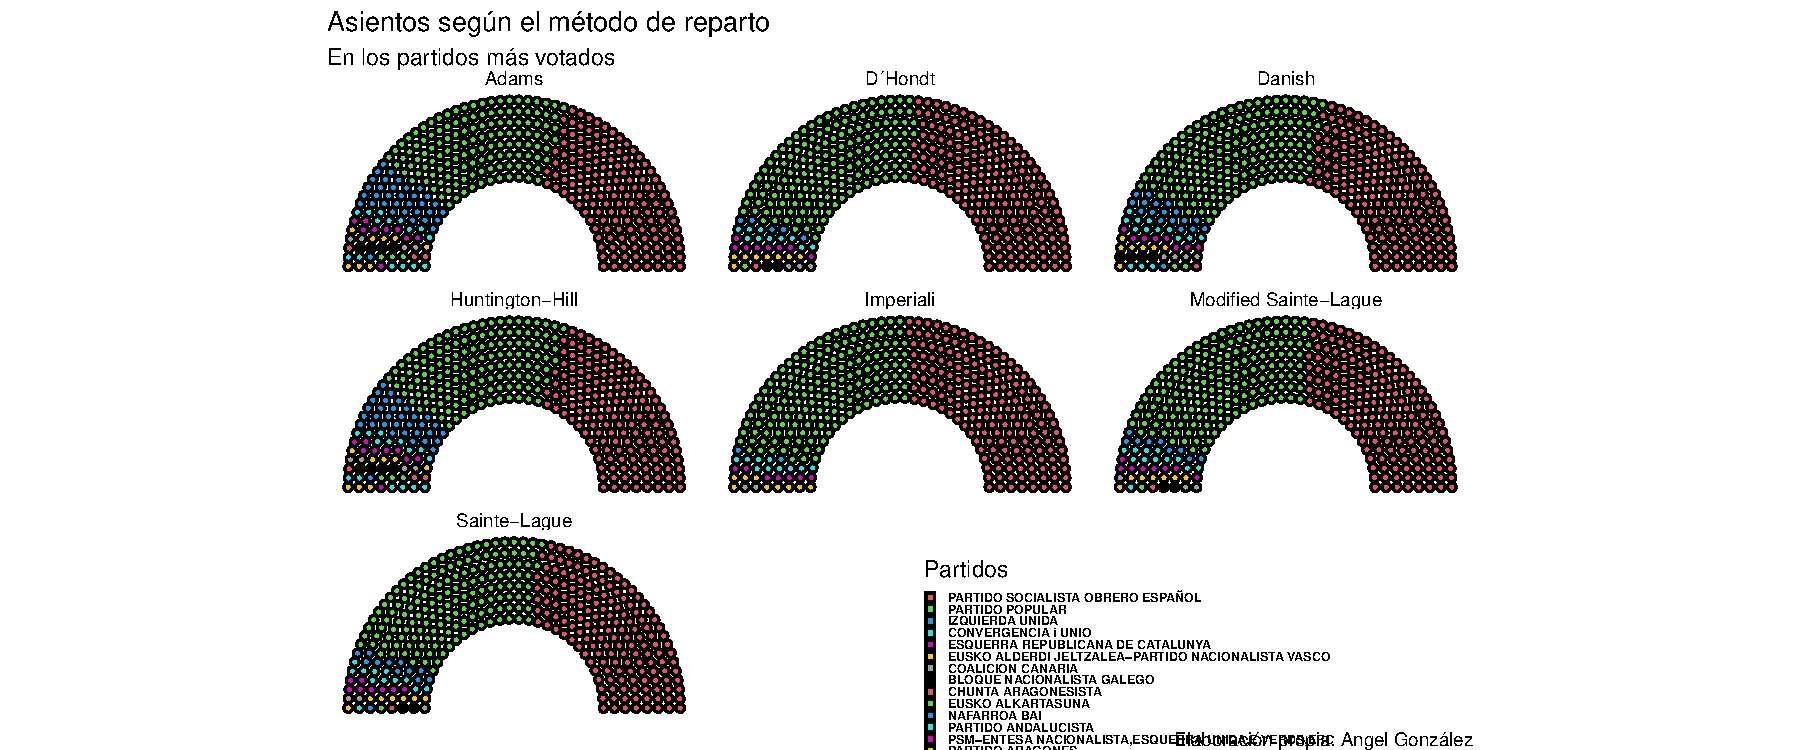
\includegraphics[width=0.95\linewidth]{figurasR/unnamed-chunk-83-1} \end{center}

\begin{center}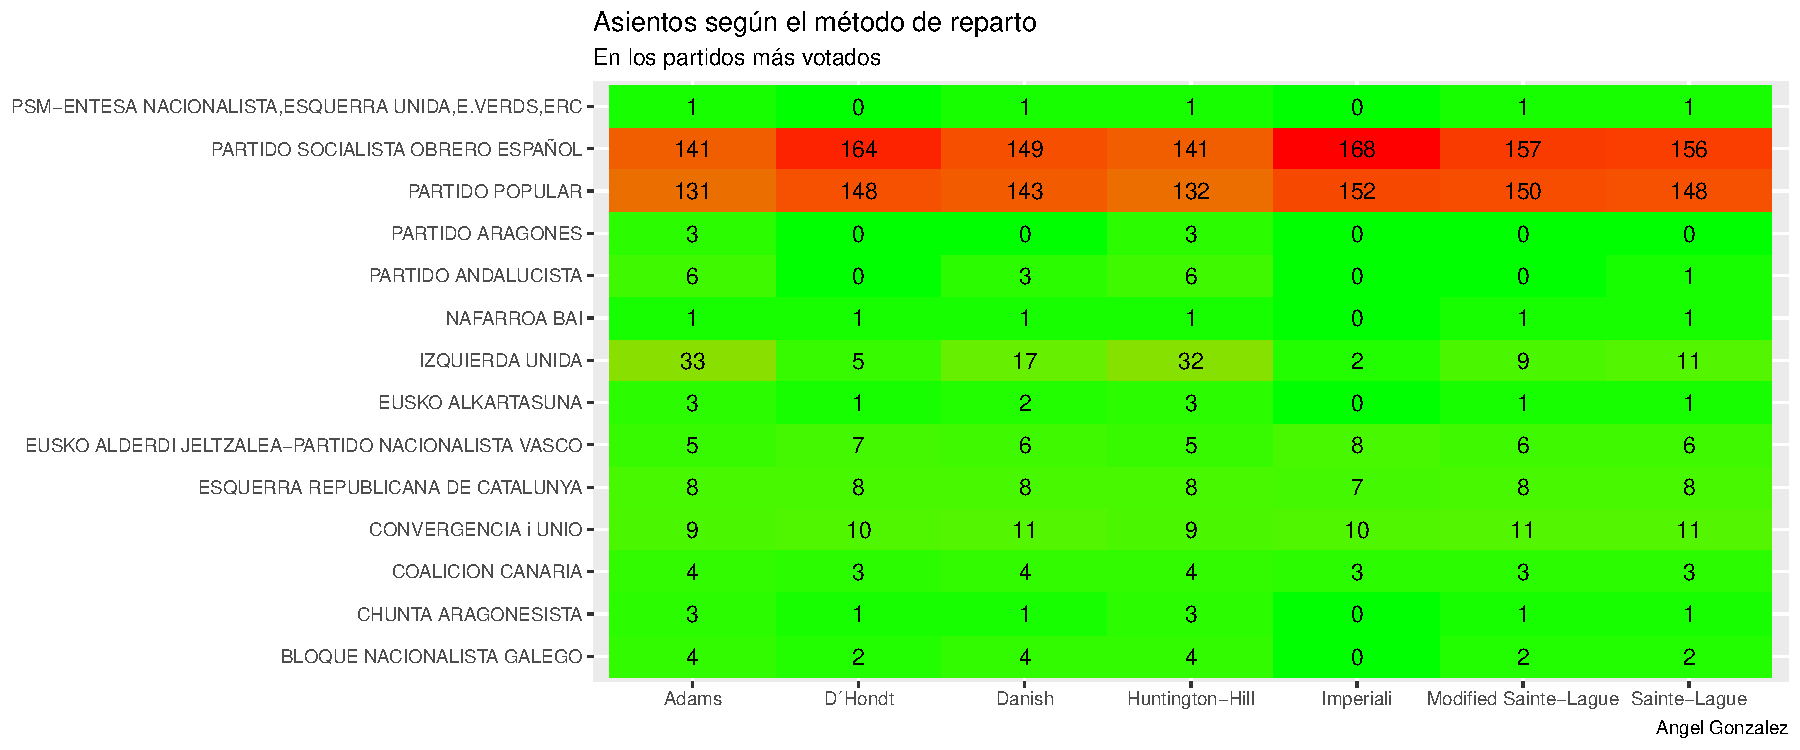
\includegraphics[width=0.95\linewidth]{figurasR/unnamed-chunk-83-2} \end{center}

\begin{center}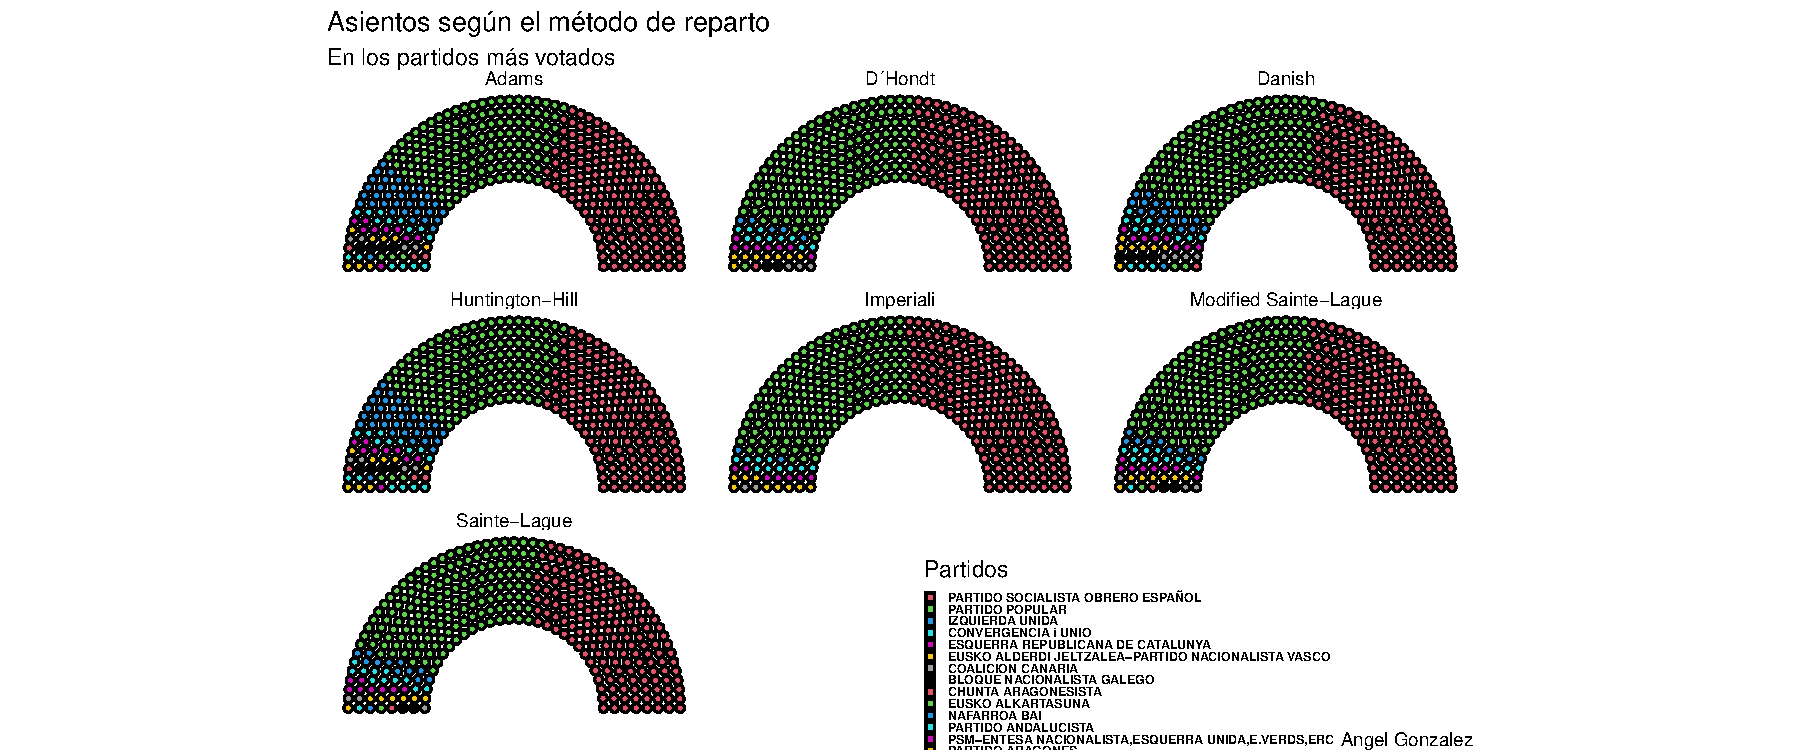
\includegraphics[width=0.95\linewidth]{figurasR/unnamed-chunk-83-3} \end{center}

En estas elecciones del año 2004 volvemos a ver unas elecciones con un
claro bipartidismo y con una diferencia de escaños entre partidos cada
vez menor, en estas elecciones el partido más votado cambia y el
\emph{PSOE} obtiene los mayores votos, seguido del \emph{PP} que pierde
la mayoría absoluta según D´Hont que tenía en las anteriores elecciones.
En ningún método el PSOE alcanzaría la mayoría absoluta por lo que
deberá de realizar alianzas con otros partidos para así alcanzar la
mayoría absoluta, si optásemos por los métodos mas proporcionales
veríamos una reducción muy significativa de la diferencia de escaños
entre partidos que pasaría de una diferencia de 16 escaños a 6 escaños
en el caso de optar por el método Danish, en cambio el partido más
castigado por el método D´Hondt, Izquierda Unida, hasta podría ver
duplicado o triplicado su presencia en el congreso.

\hypertarget{disproporcionalidad-8}{%
\subsubsection{Disproporcionalidad}\label{disproporcionalidad-8}}

\begin{center}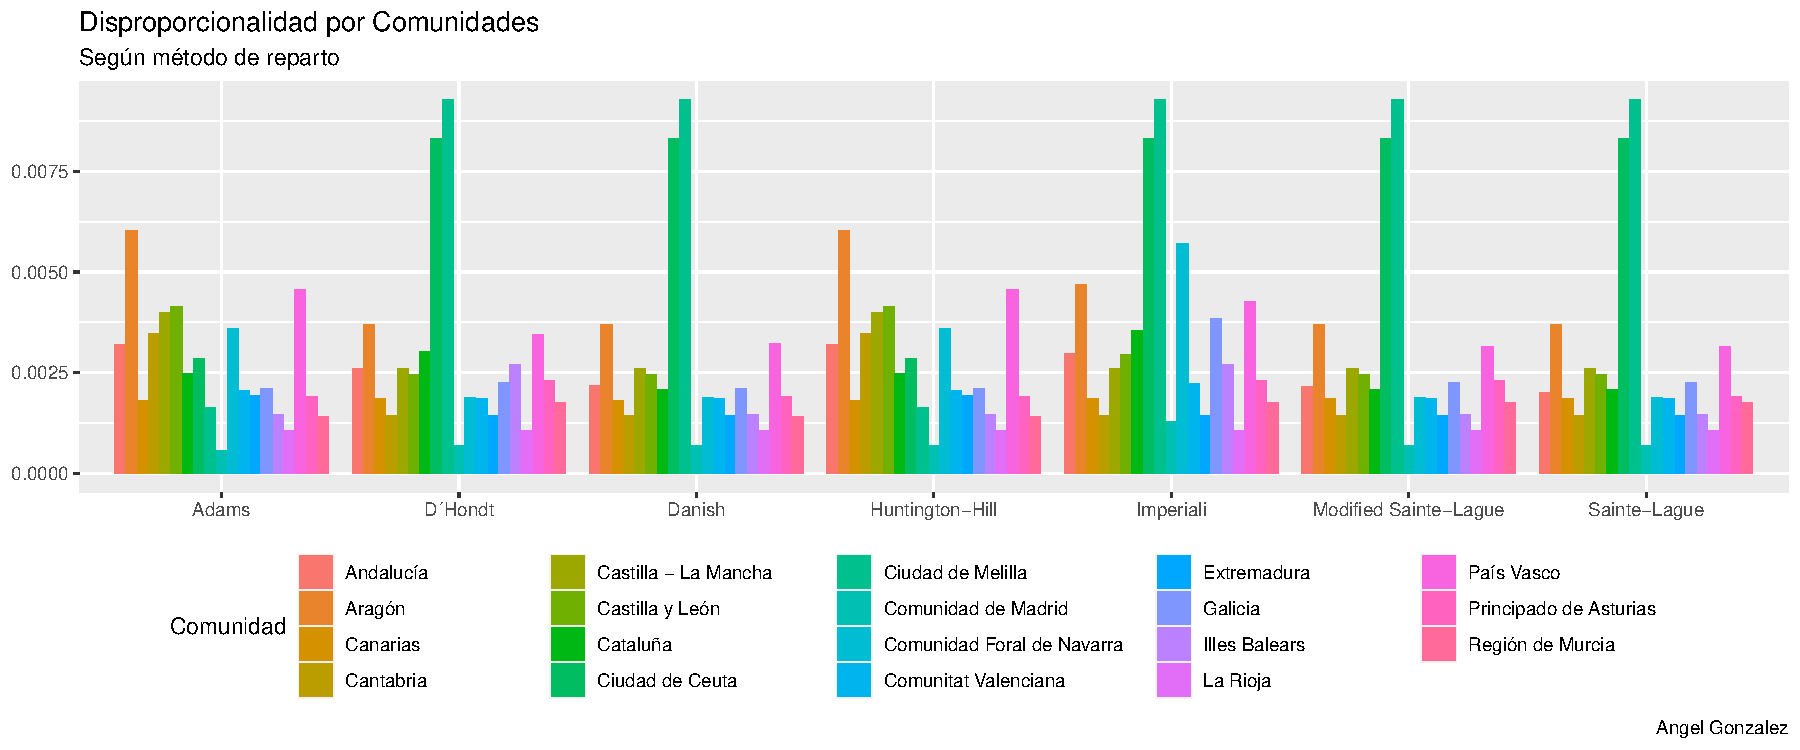
\includegraphics[width=0.95\linewidth]{figurasR/unnamed-chunk-84-1} \end{center}

\begin{center}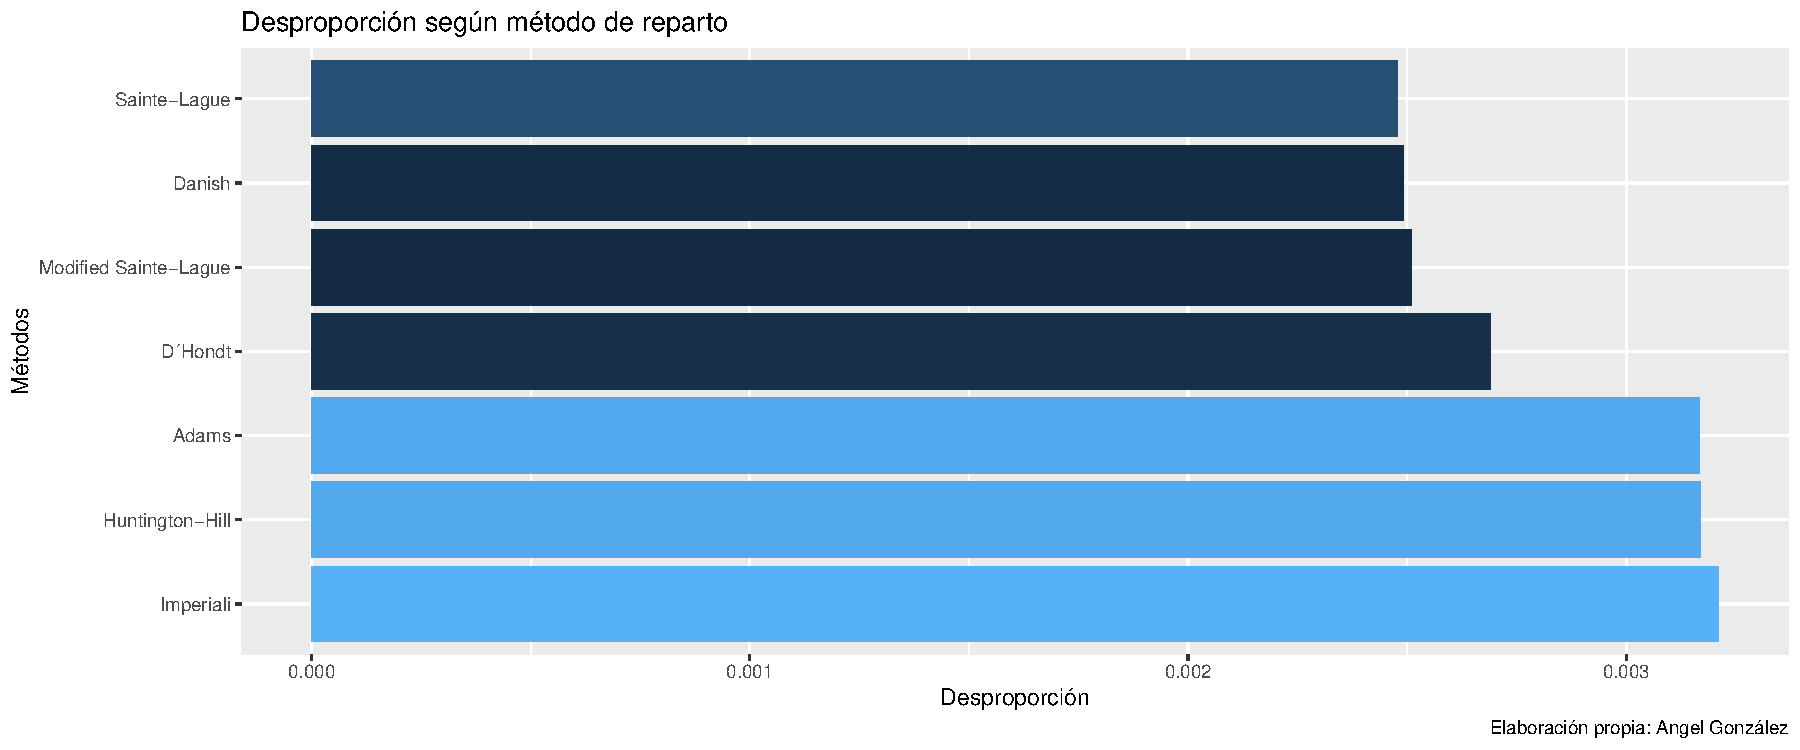
\includegraphics[width=0.95\linewidth]{figurasR/unnamed-chunk-84-2} \end{center}

Según el gráfico anterior por comunidades sigue la tónica general de las
anteriores elecciones, únicamente podemos apreciar en estas elecciones
una reducción de la disproporciorcionalidad entre comunidades, es decir,
una menor diferencia de disproporcionalidad entre ellas. En el caso de
agrupar la disproporción por métodos observamos que el método Imperiali
vuelve a ser el más disproporcionado este año mientras que en la parte
de los métodos mas proporcionados el método mejor sería el Sainte-Lague,
el método utilizado en España sigue siendo un método que se encuentra en
el medio, no siendo ni bueno ni malo.

\hypertarget{auxf1o-2008}{%
\section{Año 2008}\label{auxf1o-2008}}

\hypertarget{comparativa-entre-muxe9todos-9}{%
\subsection{Comparativa entre
métodos}\label{comparativa-entre-muxe9todos-9}}

\hypertarget{votos-obtenidos-9}{%
\subsubsection{Votos obtenidos}\label{votos-obtenidos-9}}

\begin{center}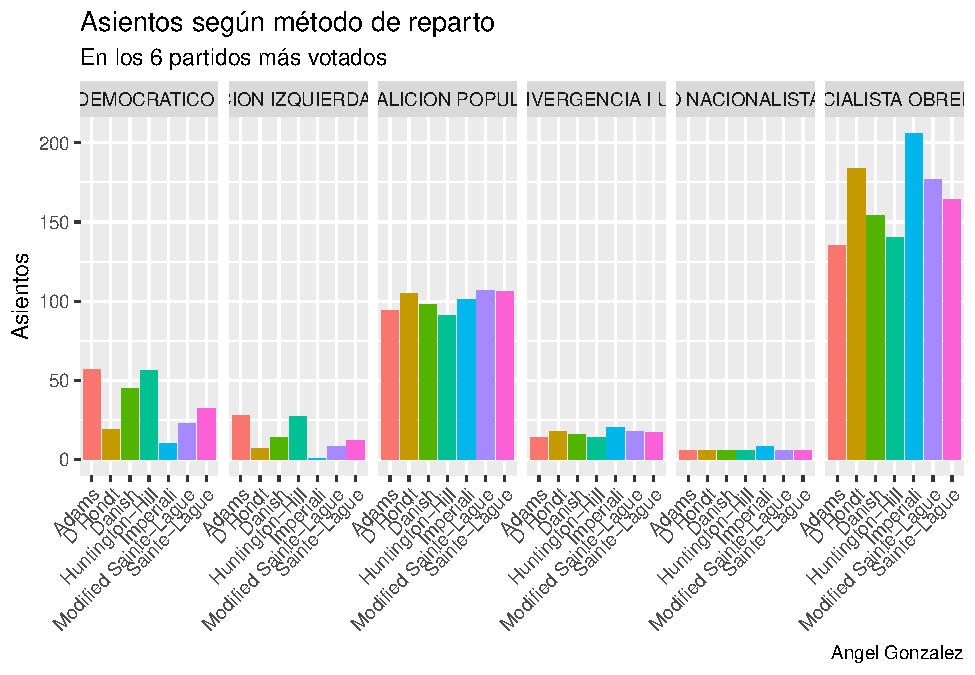
\includegraphics[width=0.95\linewidth]{figurasR/unnamed-chunk-92-1} \end{center}

\begin{center}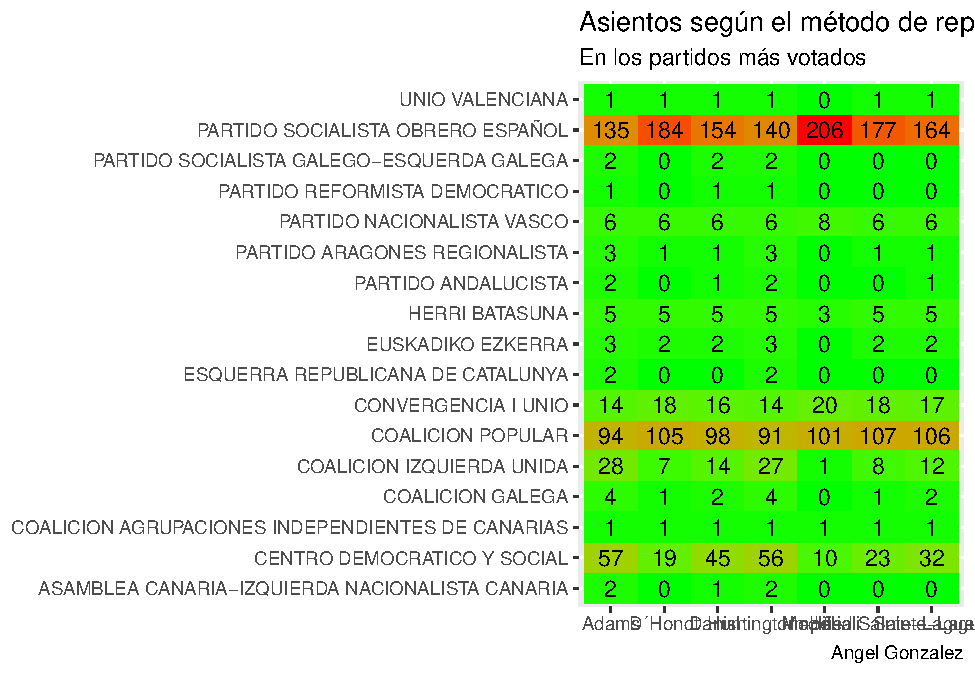
\includegraphics[width=0.95\linewidth]{figurasR/unnamed-chunk-92-2} \end{center}

\begin{center}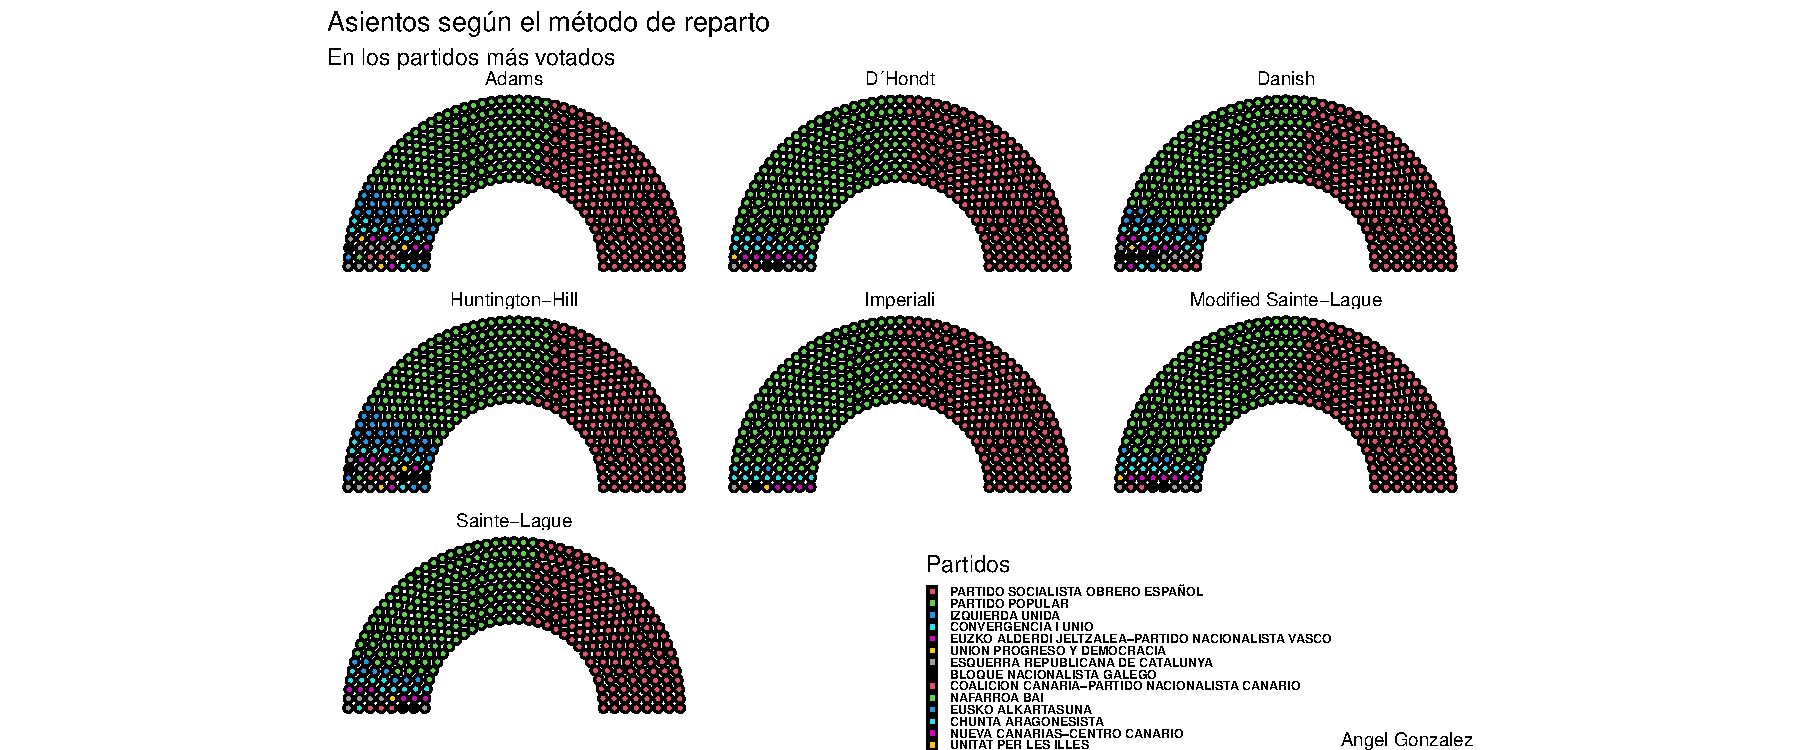
\includegraphics[width=0.95\linewidth]{figurasR/unnamed-chunk-92-3} \end{center}

En estos comicios del año 2008 no hay diferencias significativas en
términos de escaños, sigue un claro bipartidismo con dos partidos
hegemónicos, en primer lugar el más votado en estas elecciones que sigue
siendo el \emph{PSOE} seguido por el \emph{PP}, la diferencia de escaños
entre ellos continúa siendo prácticamente la misma pero en este año el
bipartidismo es cada vez más pronunciado, aumentando ambos partidos su
presencia en el congreso. Para el partido más votado únicamente en un
caso podría obtener la mayoría absoluta, que sería en el caso de optar
por el método Imperiali, una mayoría absoluta justa al llegar sólo a los
175 escaños. Utilizando los métodos de reparto más proporcionales como
son el Danish y el Sainte-Lague la diferencia entre los partidos más
votados se reduciría a la vez que obtendrían un menor número de escaños,
el partido más perjudicado sigue siendo Izquierda Unida que podría en
este año hasta mas que quintuplicar su presencia en el congreso de haber
optado por el método Danish.

\hypertarget{disproporcionalidad-9}{%
\subsubsection{Disproporcionalidad}\label{disproporcionalidad-9}}

\begin{center}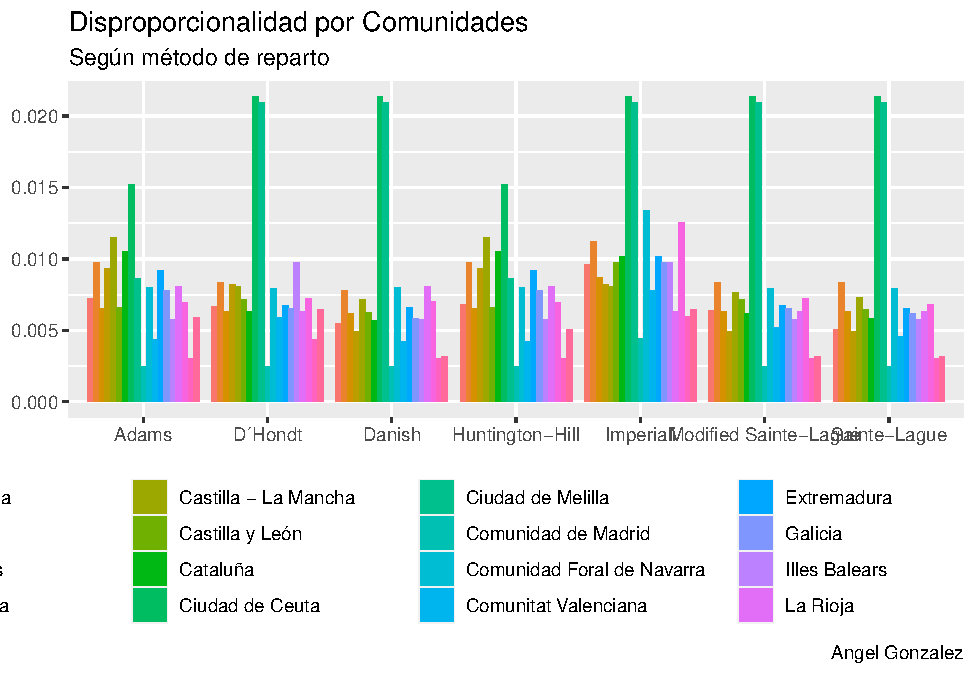
\includegraphics[width=0.95\linewidth]{figurasR/unnamed-chunk-93-1} \end{center}

\begin{center}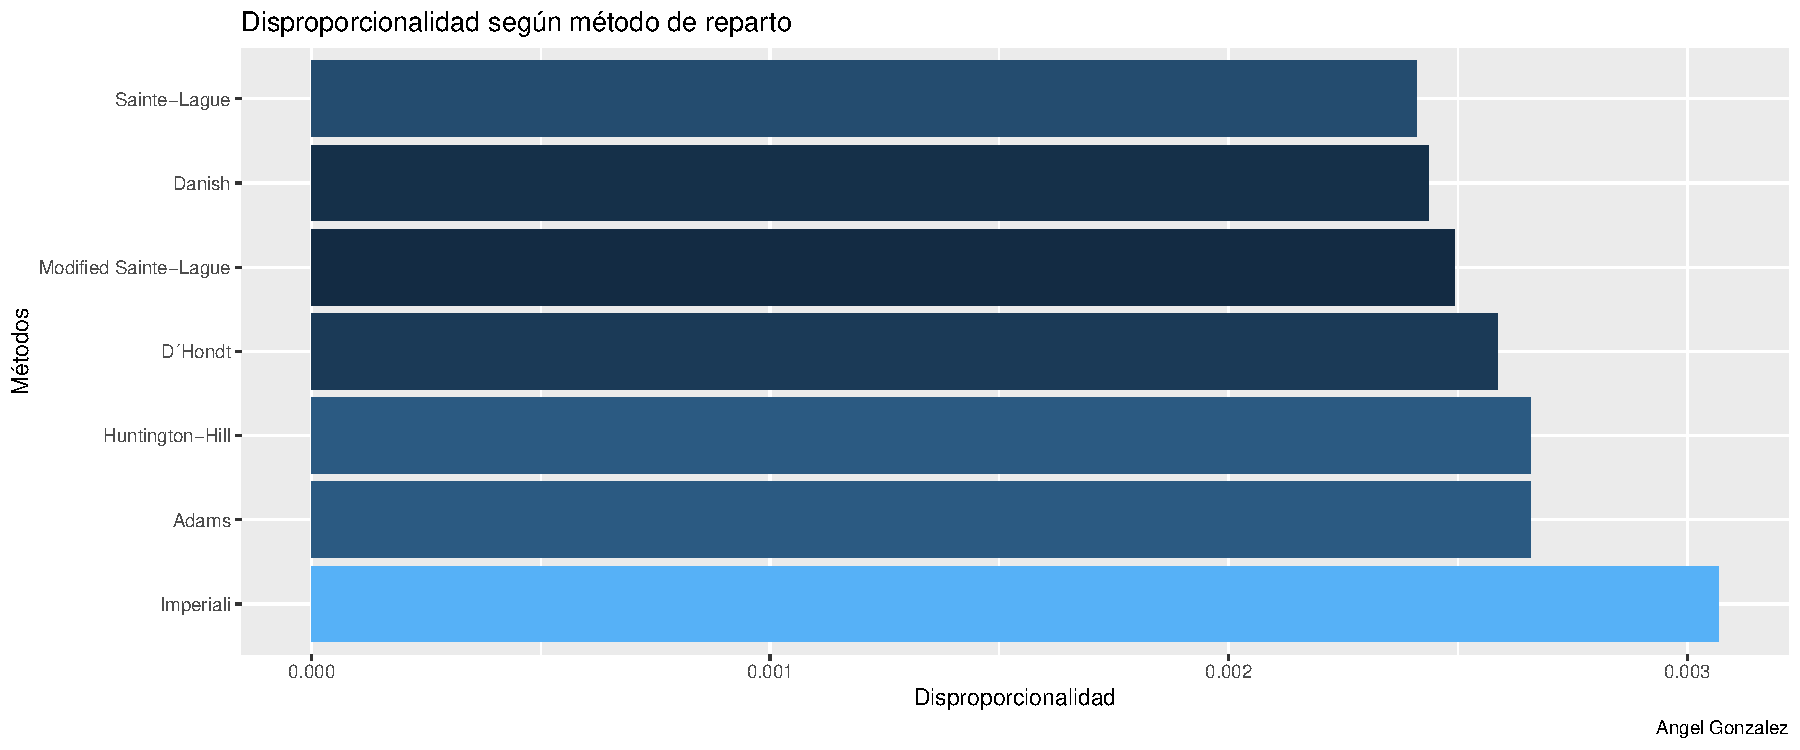
\includegraphics[width=0.95\linewidth]{figurasR/unnamed-chunk-93-2} \end{center}

Este es un año que se puede observar una mayor igualdad en el caso de
las disproporcionalidades, las comunidades no tienen una gran diferencia
de proporcionalidad entre ellas y además no encontramos grandes
diferencias entre los métodos. Si observamos la gráfica de la
disproporcionalidad según el método de reparto es llamativo este año que
únicamente tenemos un método especialmente dispropocionado que es el
Imperiali, en cambio todos los demás métodos están en un mismo nivel con
una baja diferencia entre ellos, el mejor método en estas elecciones
vuelve a ser el método de Sainte-Lague, el método D´Hont utilizado en
España no presenta diferencias y se encuentra en un nivel medio-alto de
disproporcionalidad entre todos los métodos analizados.

\hypertarget{auxf1o-2011}{%
\section{Año 2011}\label{auxf1o-2011}}

\hypertarget{comparativa-entre-muxe9todos-10}{%
\subsection{Comparativa entre
métodos}\label{comparativa-entre-muxe9todos-10}}

\hypertarget{votos-obtenidos-10}{%
\subsubsection{Votos obtenidos}\label{votos-obtenidos-10}}

\begin{center}\includegraphics[width=0.95\linewidth]{figurasR/unnamed-chunk-101-1} \end{center}

\begin{center}\includegraphics[width=0.95\linewidth]{figurasR/unnamed-chunk-101-2} \end{center}

\begin{center}\includegraphics[width=0.95\linewidth]{figurasR/unnamed-chunk-101-3} \end{center}

Este año 2011 podemos considerarlo como el primer año en el que aunque
siga sucediendo un claro bipartidismo empiezan a surgir partidos
medianos con cada vez más presencia en el congreso, en este año es la
aparición de UPyD. El partido más votado en estas elecciones es el
Partido Popular, que además obtiene la mayoría absoluta de forma holgada
según el método D´Hondt utilizado en España, le sigue el PSOE a una
diferencia muy significativa, casi duplica la presencia en el congreso
del PP respecto al PSOE. Si observamos los otros métodos propuestos
vemos que el PP en el caso del método Danish no llegaría a obtener la
mayoría absoluta pero si utilizásemos el método de Sainte-Lague sí que
alcanzaríamos la mayoría absoluta con 176 escaños. Los partidos más
perjudicados por utilizar el método D´Hont son en estas elecciones UPyD
y IU, los cuales de haber optado por el método Danish podrían duplicar
su presencia en el congreso. Es llamativo el resultado de las elecciones
según el método Adams y Huntington-Hill, son métodos que dan escaños a
los partidos con menos votos en detrimento de los partidos más votados,
en estas elecciones vemos como el resultado cambiaría radicalmente, el
PP de ser el partido más votado con mucha diferencia pasaría a reducir
la diferencia de escaños a la mitad pero la diferencia más notoria está
en los partidos medianos UPyD y IU, que pasarían de 5 a 41 escaños y de
11 a 54 escaños respectivamente.

\hypertarget{disproporcionalidad-10}{%
\subsubsection{Disproporcionalidad}\label{disproporcionalidad-10}}

\begin{center}\includegraphics[width=0.95\linewidth]{figurasR/unnamed-chunk-102-1} \end{center}

\begin{center}\includegraphics[width=0.95\linewidth]{figurasR/unnamed-chunk-102-2} \end{center}

Observando el gráfico de la disproporcionalidad entre comunidades vemos
como este año particularmente el comportamiento general de todos los
métodos es similar a diferencia de las anteriores elecciones en donde
los métodos Adams y Huntington-Hill presentaban un comportamiento
distinto respecto a los restantes métodos, este año el comportamiento de
todos los métodos es similar.

Si observamos la disproporcionalidad según el método de reparto volvemos
a observar dos grupos bien diferenciados, uno en el que hay una gran
disproporcionalidad, donde estarían los métodos Huntington-Hill, Adams e
Imperiali, y otro grupo con los restantes métodos con una
proporcionalidad baja. El método utilizado en España se encontraría en
el grupo de disproporcionalidad baja pero con el inconveniente de ser el
peor clasificado en ese grupo, el mejor método estas elecciones es el
Danish.

\hypertarget{auxf1o-2015}{%
\section{Año 2015}\label{auxf1o-2015}}

\hypertarget{comparativa-entre-muxe9todos-11}{%
\subsection{Comparativa entre
métodos}\label{comparativa-entre-muxe9todos-11}}

\hypertarget{votos-obtenidos-11}{%
\subsubsection{Votos obtenidos}\label{votos-obtenidos-11}}

\begin{center}\includegraphics[width=0.95\linewidth]{figurasR/unnamed-chunk-110-1} \end{center}

\begin{center}\includegraphics[width=0.95\linewidth]{figurasR/unnamed-chunk-110-2} \end{center}

\begin{center}\includegraphics[width=0.95\linewidth]{figurasR/unnamed-chunk-110-3} \end{center}

En estas elecciones del 2014 ya vemos como habíamos predicho en las
anteriores que el bipartidismo que veíamos omnipresente en todas las
elecciones anteriores ahora ya no ocurre, es el primer año en el que se
puede afirmar que ya no hay bipartidismo. El partido más votado es el
\emph{Partido Popular} seguido por el \emph{PSOE}, pero ya vemos que
este año aparecen dos nuevos partidos medianos, que son Podemos y
Ciudadanos. El partido más votado no obtiene la mayoría absoluta en
ningún método, es interesante observar como entre Podemos y Ciudadanos
en el caso de utilizar el método D´Hondt el primero superaría en dos
escaños al segundo, mientras que de haber utilizado el método Danish
Ciudadanos superaría a Podemos en dos escaños. En el caso de optar por
el método Danish el partido más votado, el PP, perdería bastantes
escaños y su diferencia respecto al segundo se vería reducida
significativamente, en el caso de los partidos medianos verían su
presencia en el congreso aumentar levemente pero en ningún caso
supondría un cambio significativo. El partido más perjudicado este año
vuelve a ser Izquierda Unida, que podría pasar de obtener 2 escaños con
el método D´Hondt a 11 escaños con el Danish.

\hypertarget{disproporcionalidad-11}{%
\subsubsection{Disproporcionalidad}\label{disproporcionalidad-11}}

\begin{center}\includegraphics[width=0.95\linewidth]{figurasR/unnamed-chunk-111-1} \end{center}

\begin{center}\includegraphics[width=0.95\linewidth]{figurasR/unnamed-chunk-111-2} \end{center}

Según el gráfico por comunidades volvemos a ver un comportamiento
claramente distinto de los demás de los métodos Adams y Huntington-Hill,
es un año en el que la diferencia de disproporcionalidad entre las
distintas comunidades aumentan.

En el caso de la disproporción según el método de reparto este año
tenemos nuevamente dos grupos difenrenciados, en un grupo con una
disproporcionalidad alta estaría únicamente el método Imperiali y todos
los métodos restantes se encontrarían en el grupo de disproporcionalidad
baja, el mejor método este año es el Sainte-Lague y encontramos que el
método utilizado en España es el segundo peor método posible, por lo
tanto sería interesante este año utilizar otro método mejor.

\hypertarget{auxf1o-2016}{%
\section{Año 2016}\label{auxf1o-2016}}

\hypertarget{comparativa-entre-muxe9todos-12}{%
\subsection{Comparativa entre
métodos}\label{comparativa-entre-muxe9todos-12}}

\hypertarget{votos-obtenidos-12}{%
\subsubsection{Votos obtenidos}\label{votos-obtenidos-12}}

\begin{center}\includegraphics[width=0.95\linewidth]{figurasR/unnamed-chunk-119-1} \end{center}

\begin{center}\includegraphics[width=0.95\linewidth]{figurasR/unnamed-chunk-119-2} \end{center}

\begin{center}\includegraphics[width=0.95\linewidth]{figurasR/unnamed-chunk-119-3} \end{center}

En las elecciones del año 2016 vemos como se va consolidando el modelo
de las anteriores elecciones, con dos grandes partidos y dos partidos
medianos. La fuerza política más votada este año es el \emph{Partido
Popular} seguido del \emph{PSOE}, en ningún método el PP alcanzaría la
mayoría absoluta, son unas elecciones que no presentan diferencias
significativas al cambiar de método de reparto, en el caso de utilizar
el método Danish respecto al D´Hondt resultaría en un menor número de
escaños para el PP y una ligera subida de escaños de Podemos y
Ciudadanos. Son las primeras elecciones en donde el método de reparto no
cambia significativamente el reparto de escaños, es notorio que en este
año el PSOE obtenga casi los mismos votos independientemente del método
utilizado.

\hypertarget{disproporcionalidad-12}{%
\subsubsection{Disproporcionalidad}\label{disproporcionalidad-12}}

\begin{center}\includegraphics[width=0.95\linewidth]{figurasR/unnamed-chunk-120-1} \end{center}

\begin{center}\includegraphics[width=0.95\linewidth]{figurasR/unnamed-chunk-120-2} \end{center}

En la disproporcionalidad por comunidades vemos el habitual
comportamiento entre los métodos, con el método Adams y el
Huntington-Hill comportándose diferente a los demás. Respecto a las
diferencias de disproporcionalidad entre comunidades este año es
especialmente similar el comportamiento entre los distintos métodos. En
el gráfico en que comparamos los métodos de reparto el comportamiento es
similar al anterior año, con un método muy disproporcional respecto a
los demás, el método Imperiali, y los demás métodos muy similares entre
ellos siendo el mejor el método de Sainte-Lague, el método utilizado en
España, el D´Hondt, vuelve a ser el segundo peor por lo que cada vez es
más necesario proponer un cambio de método de reparto a otro más
proporcional.

\hypertarget{auxf1o-2019-abril}{%
\section{Año 2019, Abril}\label{auxf1o-2019-abril}}

\hypertarget{comparativa-entre-muxe9todos-13}{%
\subsection{Comparativa entre
métodos}\label{comparativa-entre-muxe9todos-13}}

\hypertarget{votos-obtenidos-13}{%
\subsubsection{Votos obtenidos}\label{votos-obtenidos-13}}

\begin{center}\includegraphics[width=0.95\linewidth]{figurasR/unnamed-chunk-128-1} \end{center}

\begin{center}\includegraphics[width=0.95\linewidth]{figurasR/unnamed-chunk-128-2} \end{center}

\begin{center}\includegraphics[width=0.95\linewidth]{figurasR/unnamed-chunk-128-3} \end{center}

En estas elecciones de Abril de 2019 vemos como ya no existe
bipartidismo, este año podemos agrupar a los partidos políticos en
cuatro categorías, la primera en donde hay un partido con muchos votos
con una gran diferencia de escaños respecto a los demás, que es el PSOE,
un segundo grupo en donde se encontrarían dos partidos con un número
medio-alto de escaños, que son el PP y Ciudadanos respectivamente, un
tercer grupo con un número mediano de escaños con Podemos y Vox, y un
último grupo de pocos escaños con los demás partidos. Este año tampoco
hay una diferencia significativa de haber utilizado un método de reparto
respecto a otro, no hay partidos especialmente perjudicados por la
elección del método D´Hondt, en ningún caso el partido más votado
alcanza la mayoría absoluta. De haber utilizado el método Danish el
partido que se vería más beneficiado sería Vox seguido de Ciudadanos,
partido que superaría en escaños al PP y se convertiría en la segunda
fuerza en el hemiciclo.

\hypertarget{disproporcionalidad-13}{%
\subsubsection{Disproporcionalidad}\label{disproporcionalidad-13}}

\begin{center}\includegraphics[width=0.95\linewidth]{figurasR/unnamed-chunk-129-1} \end{center}

\begin{center}\includegraphics[width=0.95\linewidth]{figurasR/unnamed-chunk-129-2} \end{center}

Este es un año en el que viendo la disproporcionalidad por comunidades
es especialmente similar independientemente del método utilizado, todos
los métodos siguen un patrón de disproporcionalidad similar, sin olvidar
el comportamiento habitual de las ciudades de Ceuta y Melilla y de la
comunidad de Madrid como la provincia más proporcionada.

Cuando comparamos la proporcionalidad según el método de reparto sucede
algo que no se había visto hasta ahora, que un método que anteriormente
a llegado a ser el más disproporcionado sucede que este año es el más
proporcionado, este método es el Huntington-Hill, en el extremo opuesto
está el método Imperiali con una diferencia bastante significativa
respecto a las demás. El método utilizado en España vuelve a ser uno de
los peores, en estas elecciones el segundo peor, parece ser un método
que no está preparado para ser óptimo en escenarios en donde no hay un
bipartidismo claro.

\hypertarget{auxf1o-2019-noviembre}{%
\section{Año 2019, Noviembre}\label{auxf1o-2019-noviembre}}

\hypertarget{comparativa-entre-muxe9todos-14}{%
\subsection{Comparativa entre
métodos}\label{comparativa-entre-muxe9todos-14}}

\hypertarget{votos-obtenidos-14}{%
\subsubsection{Votos obtenidos}\label{votos-obtenidos-14}}

\begin{center}\includegraphics[width=0.95\linewidth]{figurasR/unnamed-chunk-137-1} \end{center}

\begin{center}\includegraphics[width=0.95\linewidth]{figurasR/unnamed-chunk-137-2} \end{center}

\begin{center}\includegraphics[width=0.95\linewidth]{figurasR/unnamed-chunk-137-3} \end{center}

En esta gráfica de las elecciones de Noviembre de 2019 podemos observar
una ligera recuperación del bipartidismo en donde los dos principales
partidos vuelven a aumentar el número de escaños obtenidos y también
aumentar la diferencia en escaños respecto a los demás. Son unas
elecciones en donde hay dos partidos principales, que son el \emph{PSOE}
y el \emph{PP} respectivamente, uno medio en escaños, \emph{Vox}, y tres
partidos de un nivel medio-bajo de escaños, que son \emph{Podemos},
\emph{ERC} y \emph{Ciudadanos} respectivamente. En el caso de optar por
otro método en ninguno de ellos se alcanzaría la mayoría absoluta, hay
dos partidos perjudicados por utilizar el método D´Hondt en vez de otro
más proporcional como pueda ser el Danish, que son los partidos de
Podemos que pasarían de obtener 26 escaños a 40 y el partido Ciudadanos
que pasaría a duplicar su presencia de 10 escaños a 23.

\hypertarget{disproporcionalidad-14}{%
\subsubsection{Disproporcionalidad}\label{disproporcionalidad-14}}

\begin{center}\includegraphics[width=0.95\linewidth]{figurasR/unnamed-chunk-138-1} \end{center}

\begin{center}\includegraphics[width=0.95\linewidth]{figurasR/unnamed-chunk-138-2} \end{center}

En el gráfico por comunidades obtenemos el mismo comportamiento que en
las elecciones anteriores sin obtener una diferencia significativa.
Cuando comparamos la disproporcionalidad según el método de reparto el
método de Imperiali sigue siendo el más disproporcionado mientras que el
mejor método esta vez resulta ser el Sainte-Lague, el método D´Hondt
como hemos visto en anteriores elecciones sigue siendo el segundo peor
método posible, por lo que es necesario cada vez más plantear seriamente
un cambio de método de reparto.

\hypertarget{comparativa-entre-auxf1os}{%
\section{Comparativa entre años}\label{comparativa-entre-auxf1os}}

\begin{center}\includegraphics[width=0.95\linewidth]{figurasR/unnamed-chunk-139-1} \end{center}

\begin{center}\includegraphics[width=0.95\linewidth]{figurasR/unnamed-chunk-139-2} \end{center}

En este gráfico comparando la disproporcionalidad media por año
observamos como la disproporción desde las elecciones de 1977 hasta 1989
está en un nivel medio, a partir del año 1993 la disproporción baja,
principalmente debido a un bipartidismo más marcado, esto se mantiene
hasta el año de las elecciones de 2011, en donde empieza por primera vez
a aparecer un tercer partido que debilita el bipartidismo por lo que la
disproporcionalidad aumenta a los niveles de las primeras elecciones,
desde el año 2011 hasta ya las últimas elecciones de 2019 la
disproporcionalidad se mantiene sin mucha variación.

En el gráfico de la disproporcionalidad según el método de reparto
podemos extraer conclusiones para decidir cual método ha sido el mejor a
lo largo de todas las elecciones realizadas en España a partir de 1977,
por lo tanto sacamos estas conclusiones:

\begin{itemize}
\tightlist
\item
  El mejor método es el Saint-Lague.
\item
  El peor método es el Imperiali.
\item
  El método D´Hondt es el cuarto mejor método.
\end{itemize}

Por lo tanto al preguntarnos si el método utilizado en España es el
mejor método que se puede utilizar para el reparto de los escaños
podemos afirmar que no lo es, de hecho se sitúa en la mitad de la tabla
entre todos los métodos analizados, la característica que tiene el
método D´Hont es que se sitúa entre los métodos que benefician más a los
partidos más votados y de entre ellos es el método más proporcional, por
lo que se podría decir que es el método más proporcional entre los
métodos que ``facilitan la gobernanza''. Pero si nuestro objetivo es
obtener la máxima proporcionalidad en vez de facilitar la gobernanza
deberíamos plantear un cambio de método en primer lugar al Sainte-Lague
o al Danish, ambos métodos son casi idénticos en términos de
proporcionalidad pero el Sainte-Lague tiene una mejor característica que
el Danish, que reparte los escaños de forma que es más fácil gobernar.

\bibliography{bib/library.bib,bib/paquetes.bib}


\addcontentsline{toc}{chapter}{Bibliografía}


\end{document}
